\documentclass[12pt]{article}

\usepackage{bm}
\usepackage{amsmath}
\usepackage{amssymb}
\usepackage{cite}
\usepackage{indentfirst}
\usepackage{url}
\usepackage{graphicx}
\usepackage{pythonhighlight}

\title{Project 3 \\\vspace{1em}
\large CS 525: Deep Learning}
\author{
  Jerry Duncan \\
  jdunca51@vols.utk.edu
}
\date{March 30, 2020}
\begin{document}
\maketitle
\pagebreak

\section{Introduction}

For this project we'll be taking a look at a few different common architectures for
 classifying images as well as a variational auto encoder to see how hard it is to replicate
 images.
Specifically, I will be taking a look at all five architectures and running extensive tests on their
 loss and accuracy over fifty epochs, with each one being trained on all of the optimizers that
 keras makes available to us.
I plan on evaluating each optimizer to see which one helps us on Fashion-MNIST the best.
Afterwards, I will lay the groundwork for continuing this work by showing how to take the best
 optimizer and loss function for each architecture and test the hyperparameters for its best optimizer.


\section{Networks}

\subsection{Fully Connected Neural Network}

The first network we'll be looking at is a simple neural network that is fully connected (FCNN).
Typically these are not meant to handle image data but because the images are so small (28x28),
 and their ability to work on MNIST already, it's worth giving a three layer dense network a shot.
\begin{python}
  Dense(784, activation="tanh"),
  Dense(512, activation="sigmoid"),
  Dense(100, activation="relu"),
  Dense(10, activation="softmax")
\end{python}


\subsection{Small Convolutional Neural Network}

The second network is a small convolutional neural network (SCNN).
These types of networks are typically intended to use when working with image data so based on the literature,
 we can expect that this should outperform the FCNN, even if only marginally.
This network only has one convolutional layer which is atypical for networks in the literature,
 but because the problem is so small and simple, it's likely that we'll get somewhat decent results using it.
\begin{python}
Conv2D(40, (5, 5), activation="relu"),
MaxPooling2D(pool_size=(2, 2)),
Flatten(),
Dense(100, activation="relu"),
Dense(10, activation="softmax")
\end{python}


\subsection{Bigger Convolutional Neural Network}

The third network is a larger convolutional neural network (BCNN).
This one uses two convolutional layers and two max pooling layers before the fully connected classification layers.
We also use more filters in each of the convolutional layers to try to learn more minute features.
\begin{python}
Conv2D(48, (3, 3), activation="relu"),
MaxPooling2D(pool_size=(2, 2)),
Conv2D(96, (3, 3), activation="relu"),
MaxPooling2D(pool_size=(2, 2)),
Flatten(),
Dense(100, activation="relu"),
Dense(10, activation="softmax")
\end{python}


\subsection{My Convolutional Neural Network}

The fourth network is one that I've created on my own (MCNN).
For this architecture I've gathered inspiration from more typical architectures you'd see in the literature.
I use two convolutional layers before each max pooling layer, lower the number of filters to a more
 reasonable 32 and 64, introduce dropout after each max pooling layer to increase robustness, and
 add batch normalization in the dense layers to smooth the optimization landscape.
\begin{python}
Conv2D(32, (5, 5), activation="relu", padding="same"),
Conv2D(32, (5, 5), activation="relu", padding="same"),
MaxPooling2D(pool_size=(2, 2)),
Dropout(0.25),
Conv2D(64, (3, 3), activation="relu", padding="same"),
Conv2D(64, (3, 3), activation="relu", padding="same"),
MaxPooling2D(pool_size=(2, 2)),
Dropout(0.25),
Flatten(),
Dense(512, activation="relu"),
BatchNormalization(),
Dropout(0.5),
Dense(10, activation="softmax")
\end{python}


\subsection{Variational Auto Encoder}

The last network is one of a different type altogether and isn't used for classification at all.
Instead, it's meant to learn a compressed representation of the data that can be used to recreate it.
A variational auto encoder aims to learn a small encoding of the input data that a decoder can then use to
 recreate the input.
The use of this is that we can generate vectors in the encoding space to generate images that didn't exist in our training set.
As for the architecture of this network, it's too complex to post a keras implementation.
For our experiments, we'll be using two similarly architected models, but with different parameters.
Both have an encoder that consists of two convolutional layers and a dense one before
 the mean, variance, and z layers.
Both also have a decoder that consists of a dense layer and then two deconvolutional layers before the output.
The difference between the two models is that the first one (VAE$_1$) has half as many filters in each convolutional layer,
 a latent vector that's 5 long instead of 10, and a smaller kernel size of 3 over the 5 of the second one (VAE$_2$).

\section{Results}

\subsection{Dataset, Preprocessing and Other Hyperparameters}

The dataset that we are using is called Fashion-MNIST.
It consists of 70,000 28$\times$28 black and white images of different articles of clothing.
Before classification and training we will scale the images to be between zero and one by using min-max scaling.
The hyper parameters we will be using across every optimizer are the following:
We run each model for fifty epochs, with a batch size of 200, and the categorical crossentropy loss function.
For each optimizer, I use the stock hyperparameters.
Opting to use the ones suggested by each paper's original authors over my own ideas.


\subsection{Fully Connected Neural Network}

In Figures \ref{fig:task_1_loss_epochs}, \ref{fig:task_1_loss_time}, and \ref{fig:task_1_acc_epochs}, we can see
 the loss and accuracy during training.
Three of the optimizers seems to get a very slow start and never manage to catch back up to the other four.
The networks using the other four optimizers started to experience overfitting the further time went on.
This can especially be seen in Figure \ref{fig:task_1_acc_epochs}.

In Figure \ref{fig:task_1_cm}, we can see that the FCNN did especially poorly
 at discerning between similar clothing types.
Shirts, coats, and t-shirts/tops were all especially challenging for it.

In Table \ref{tab:FCNN} we can see the final results of our experiments on the FCNN.
Overall, most performed in the 80\% range which is solidly okay.
Adamax managed to get the best performance with 89.74\%.

\begin{figure}
  \centering
  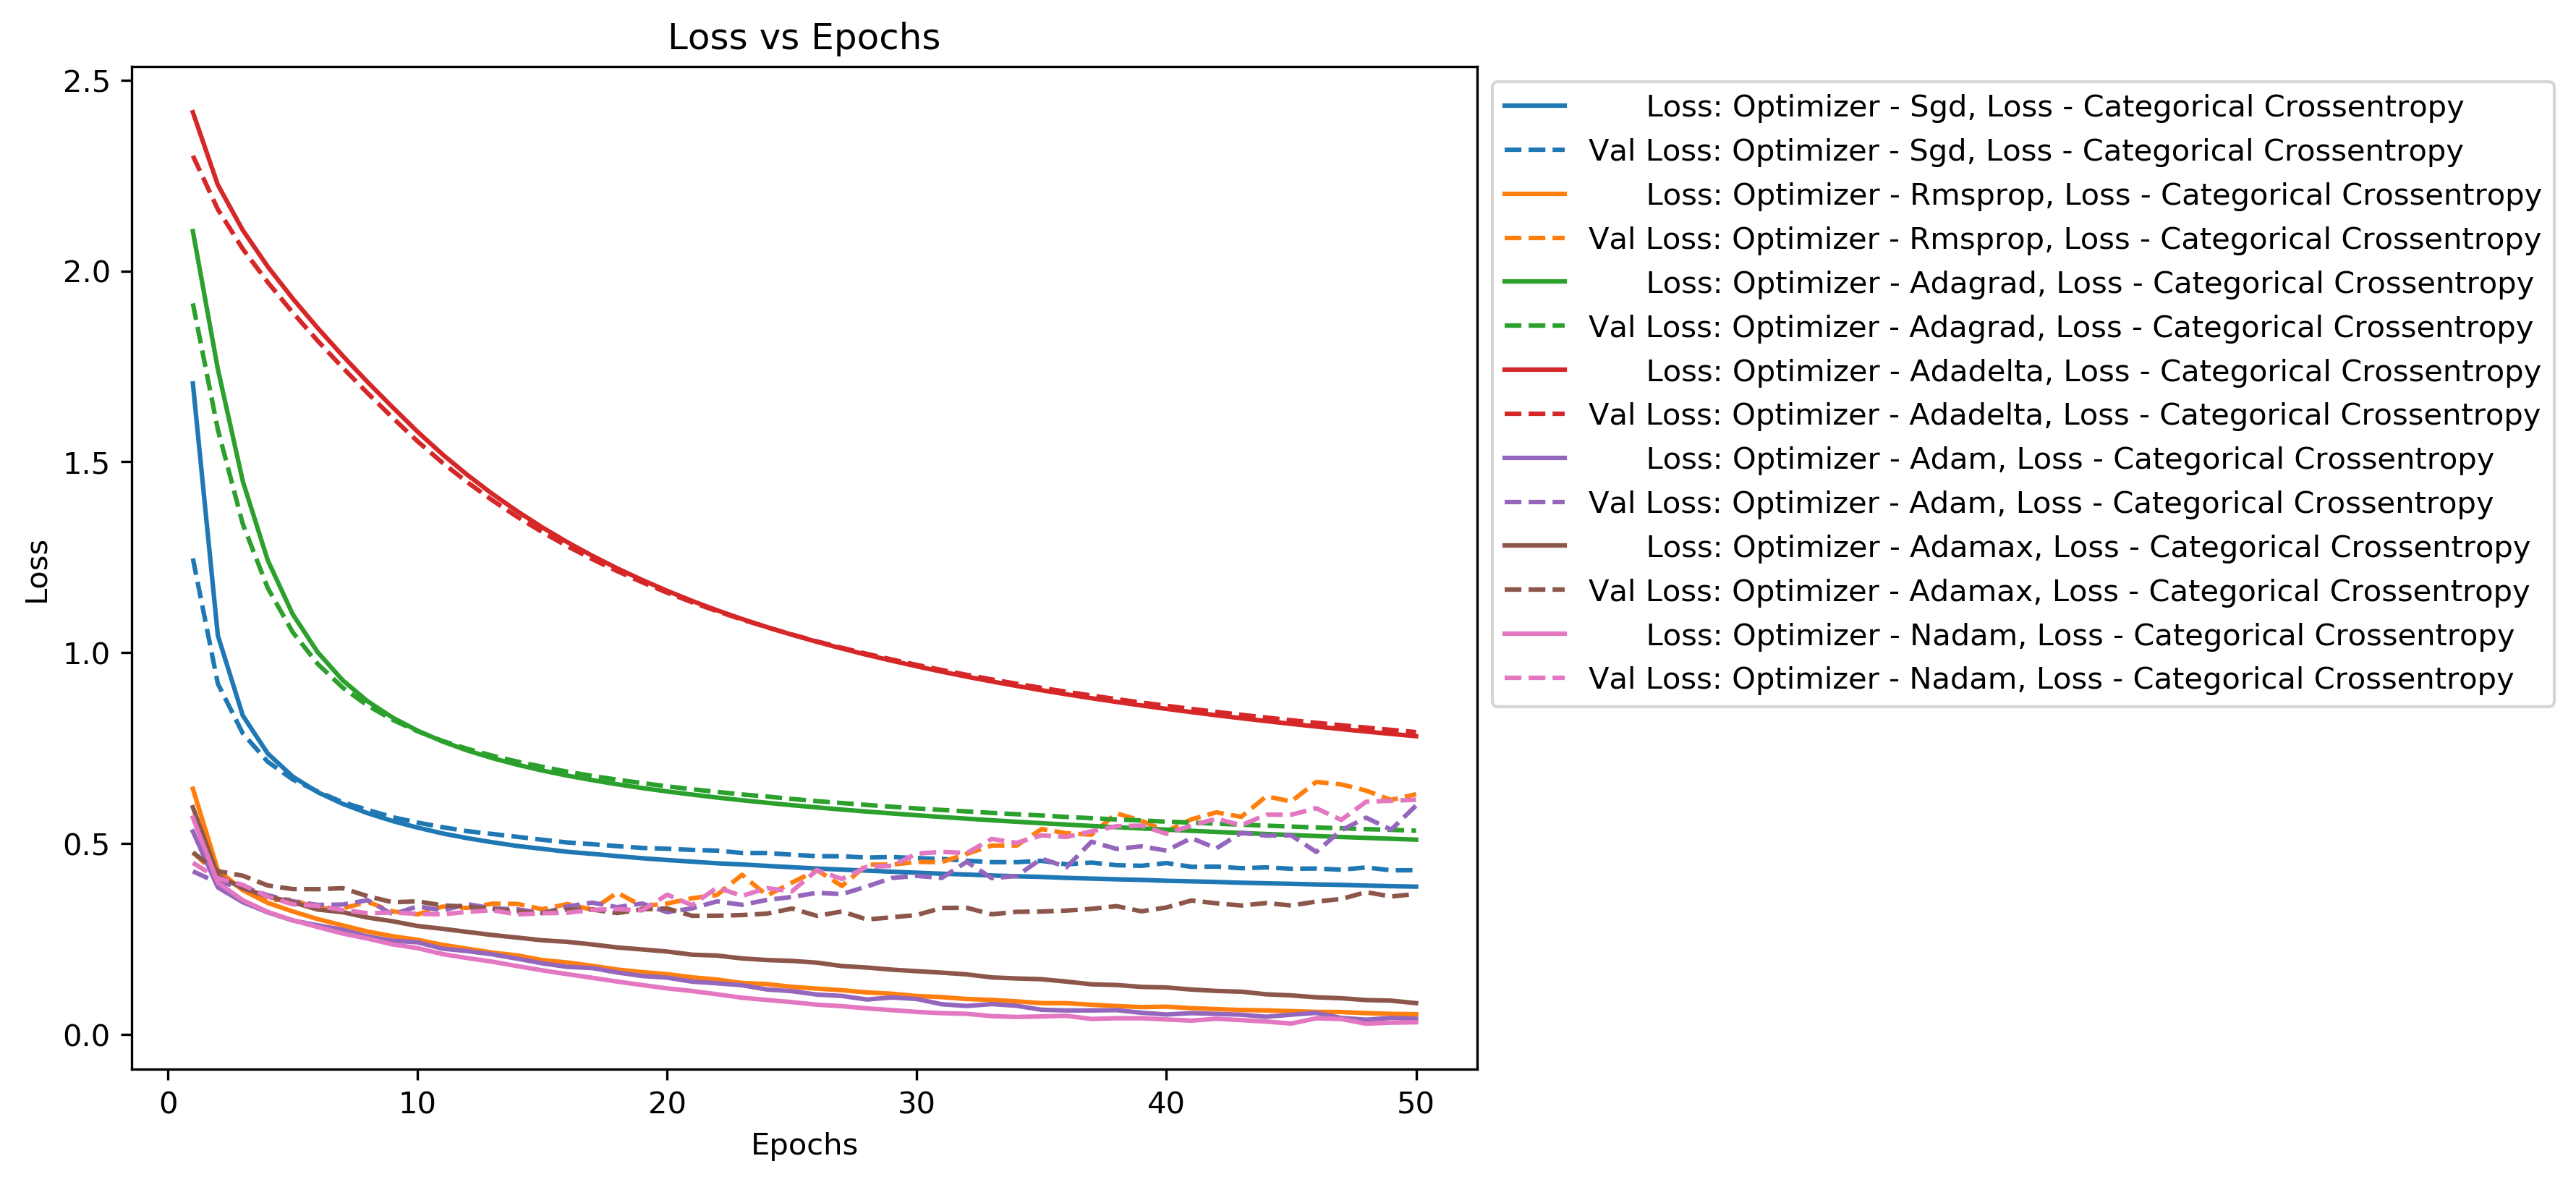
\includegraphics[width=\linewidth]{task_1_loss_epochs.png}
  \caption{Loss of FCNN using different optimizers over epochs.}
  \label{fig:task_1_loss_epochs}
\end{figure}

\begin{figure}
  \centering
  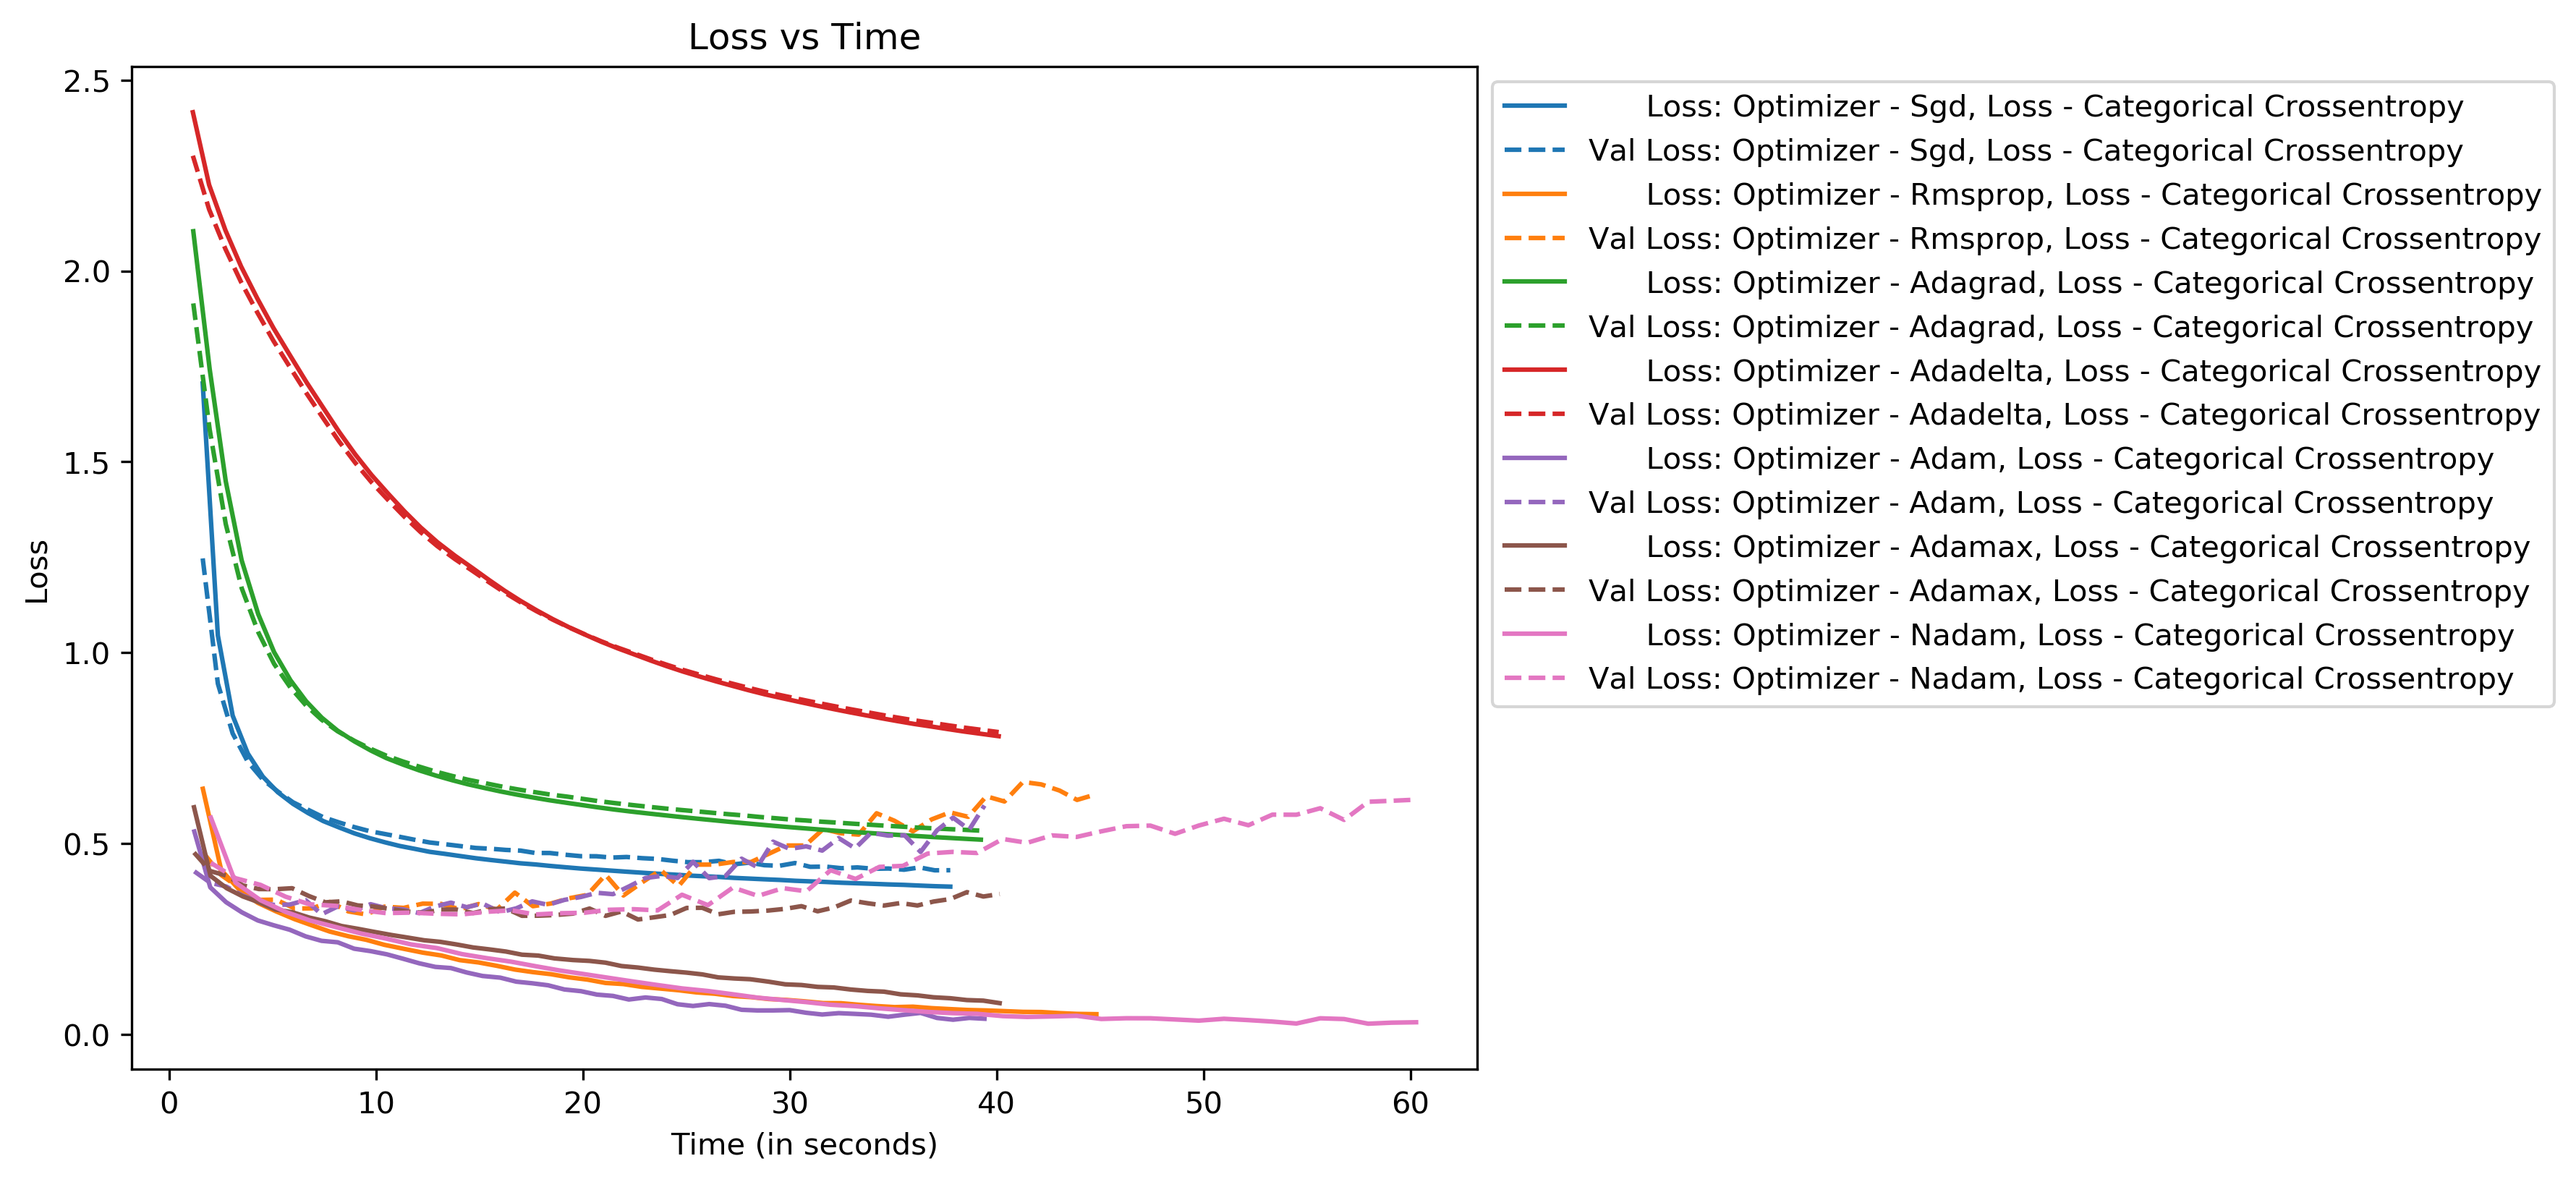
\includegraphics[width=\linewidth]{task_1_loss_time.png}
  \caption{Loss of FCNN using different optimizers over time.}
  \label{fig:task_1_loss_time}
\end{figure}

\begin{figure}
  \centering
  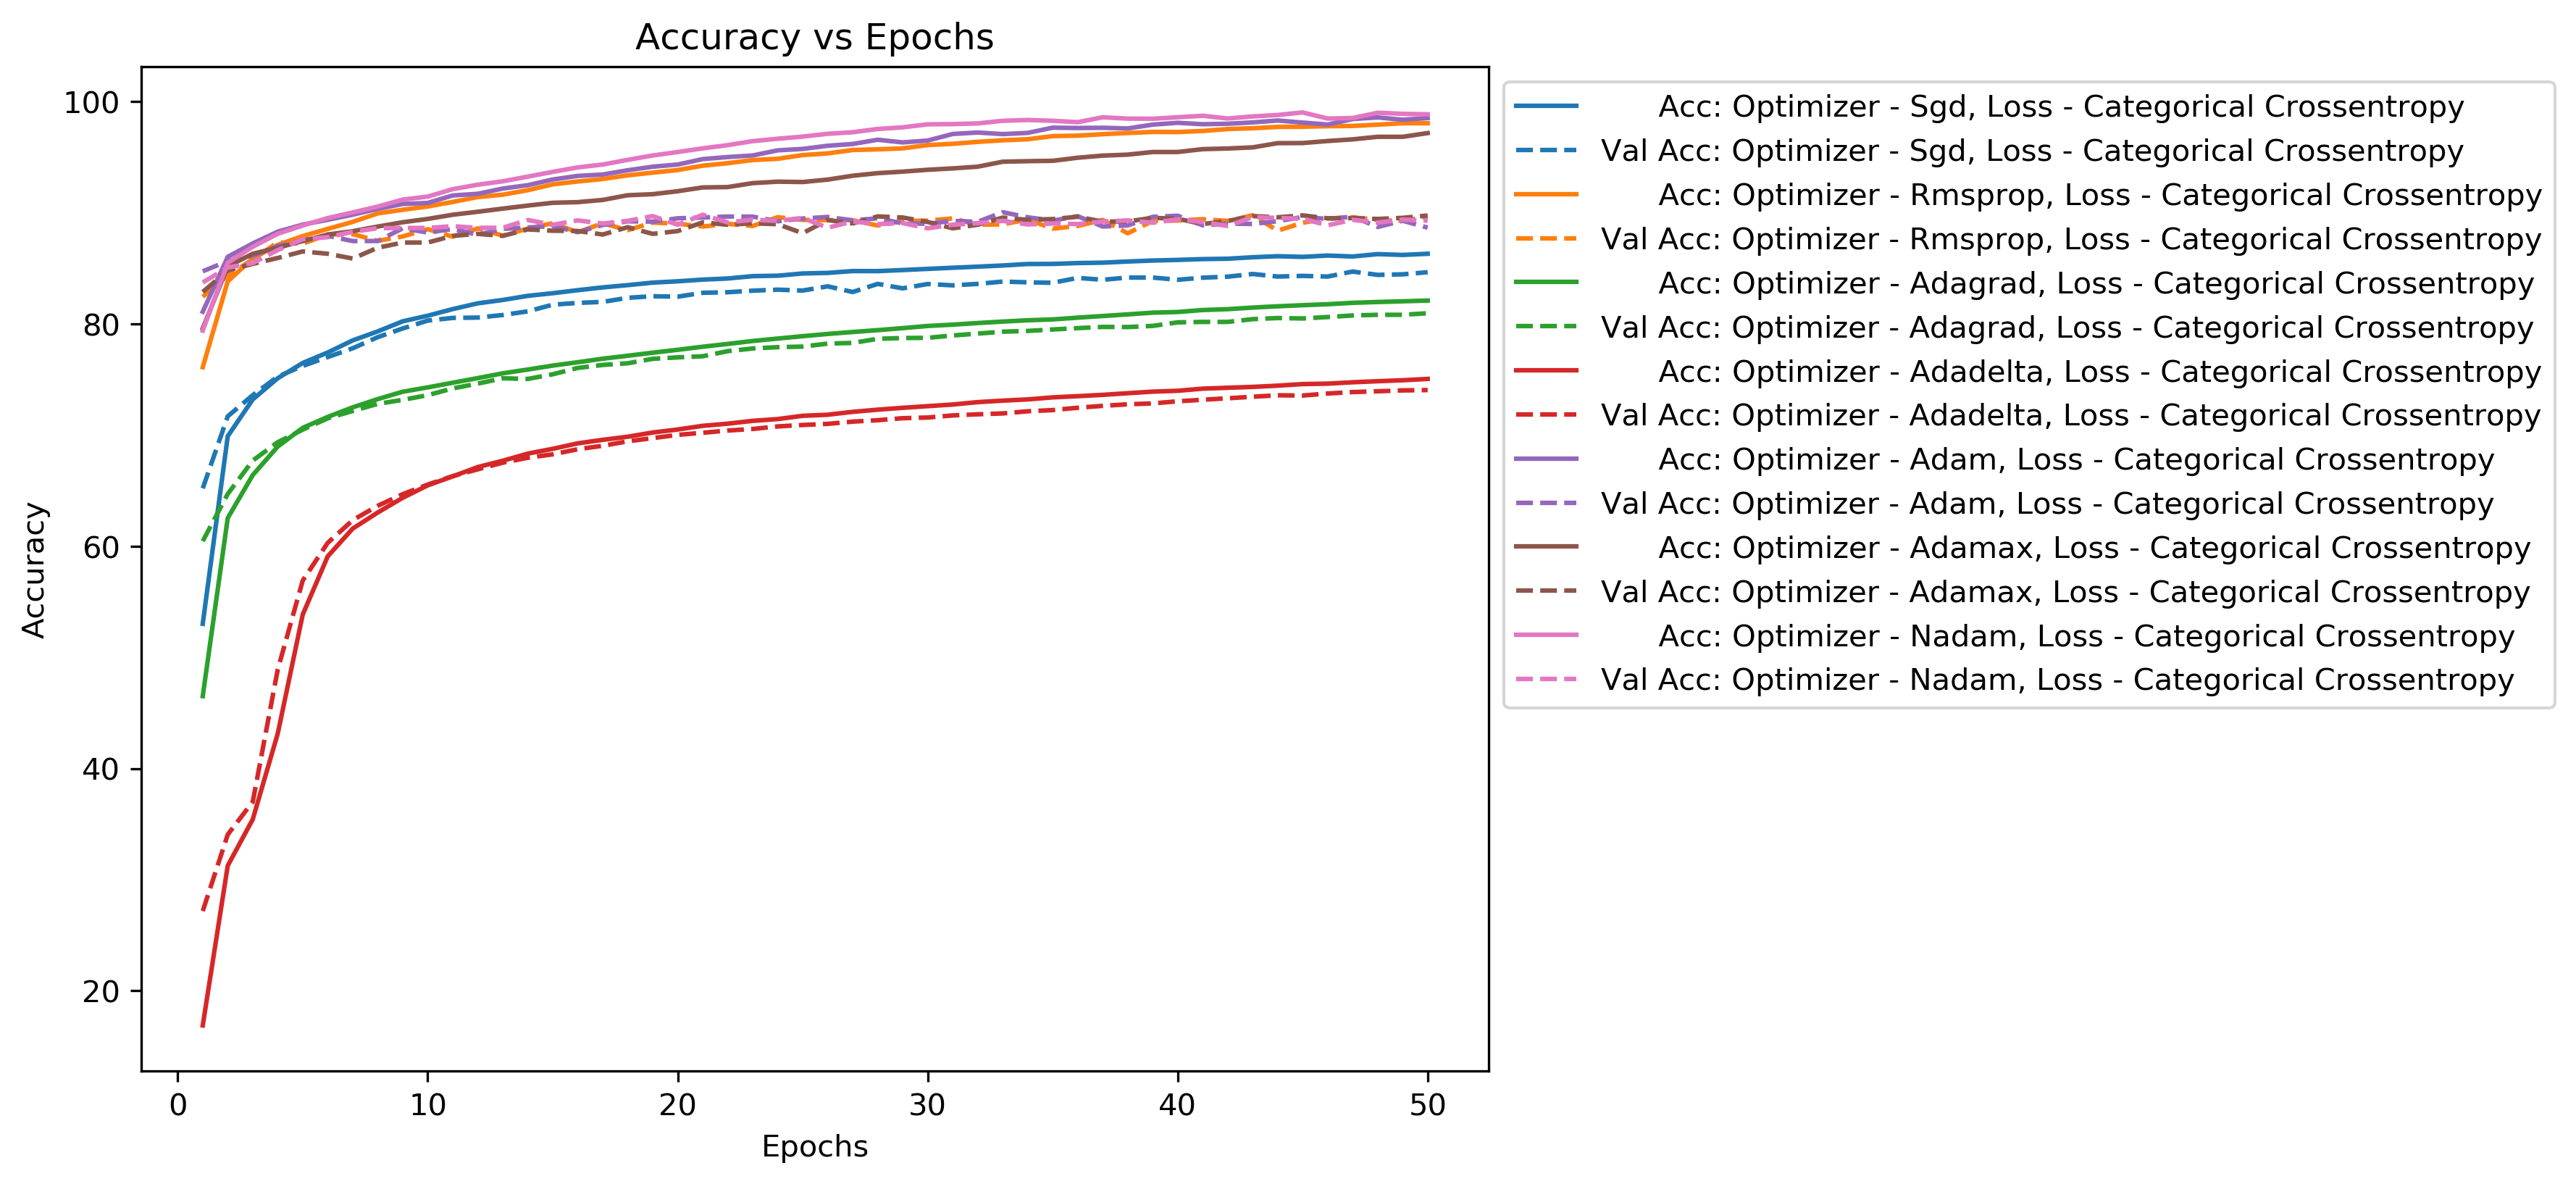
\includegraphics[width=\linewidth]{task_1_acc_epochs.png}
  \caption{Accuracy of FCNN using different optimizers over time.}
  \label{fig:task_1_acc_epochs}
\end{figure}

\begin{figure}
  \centering
  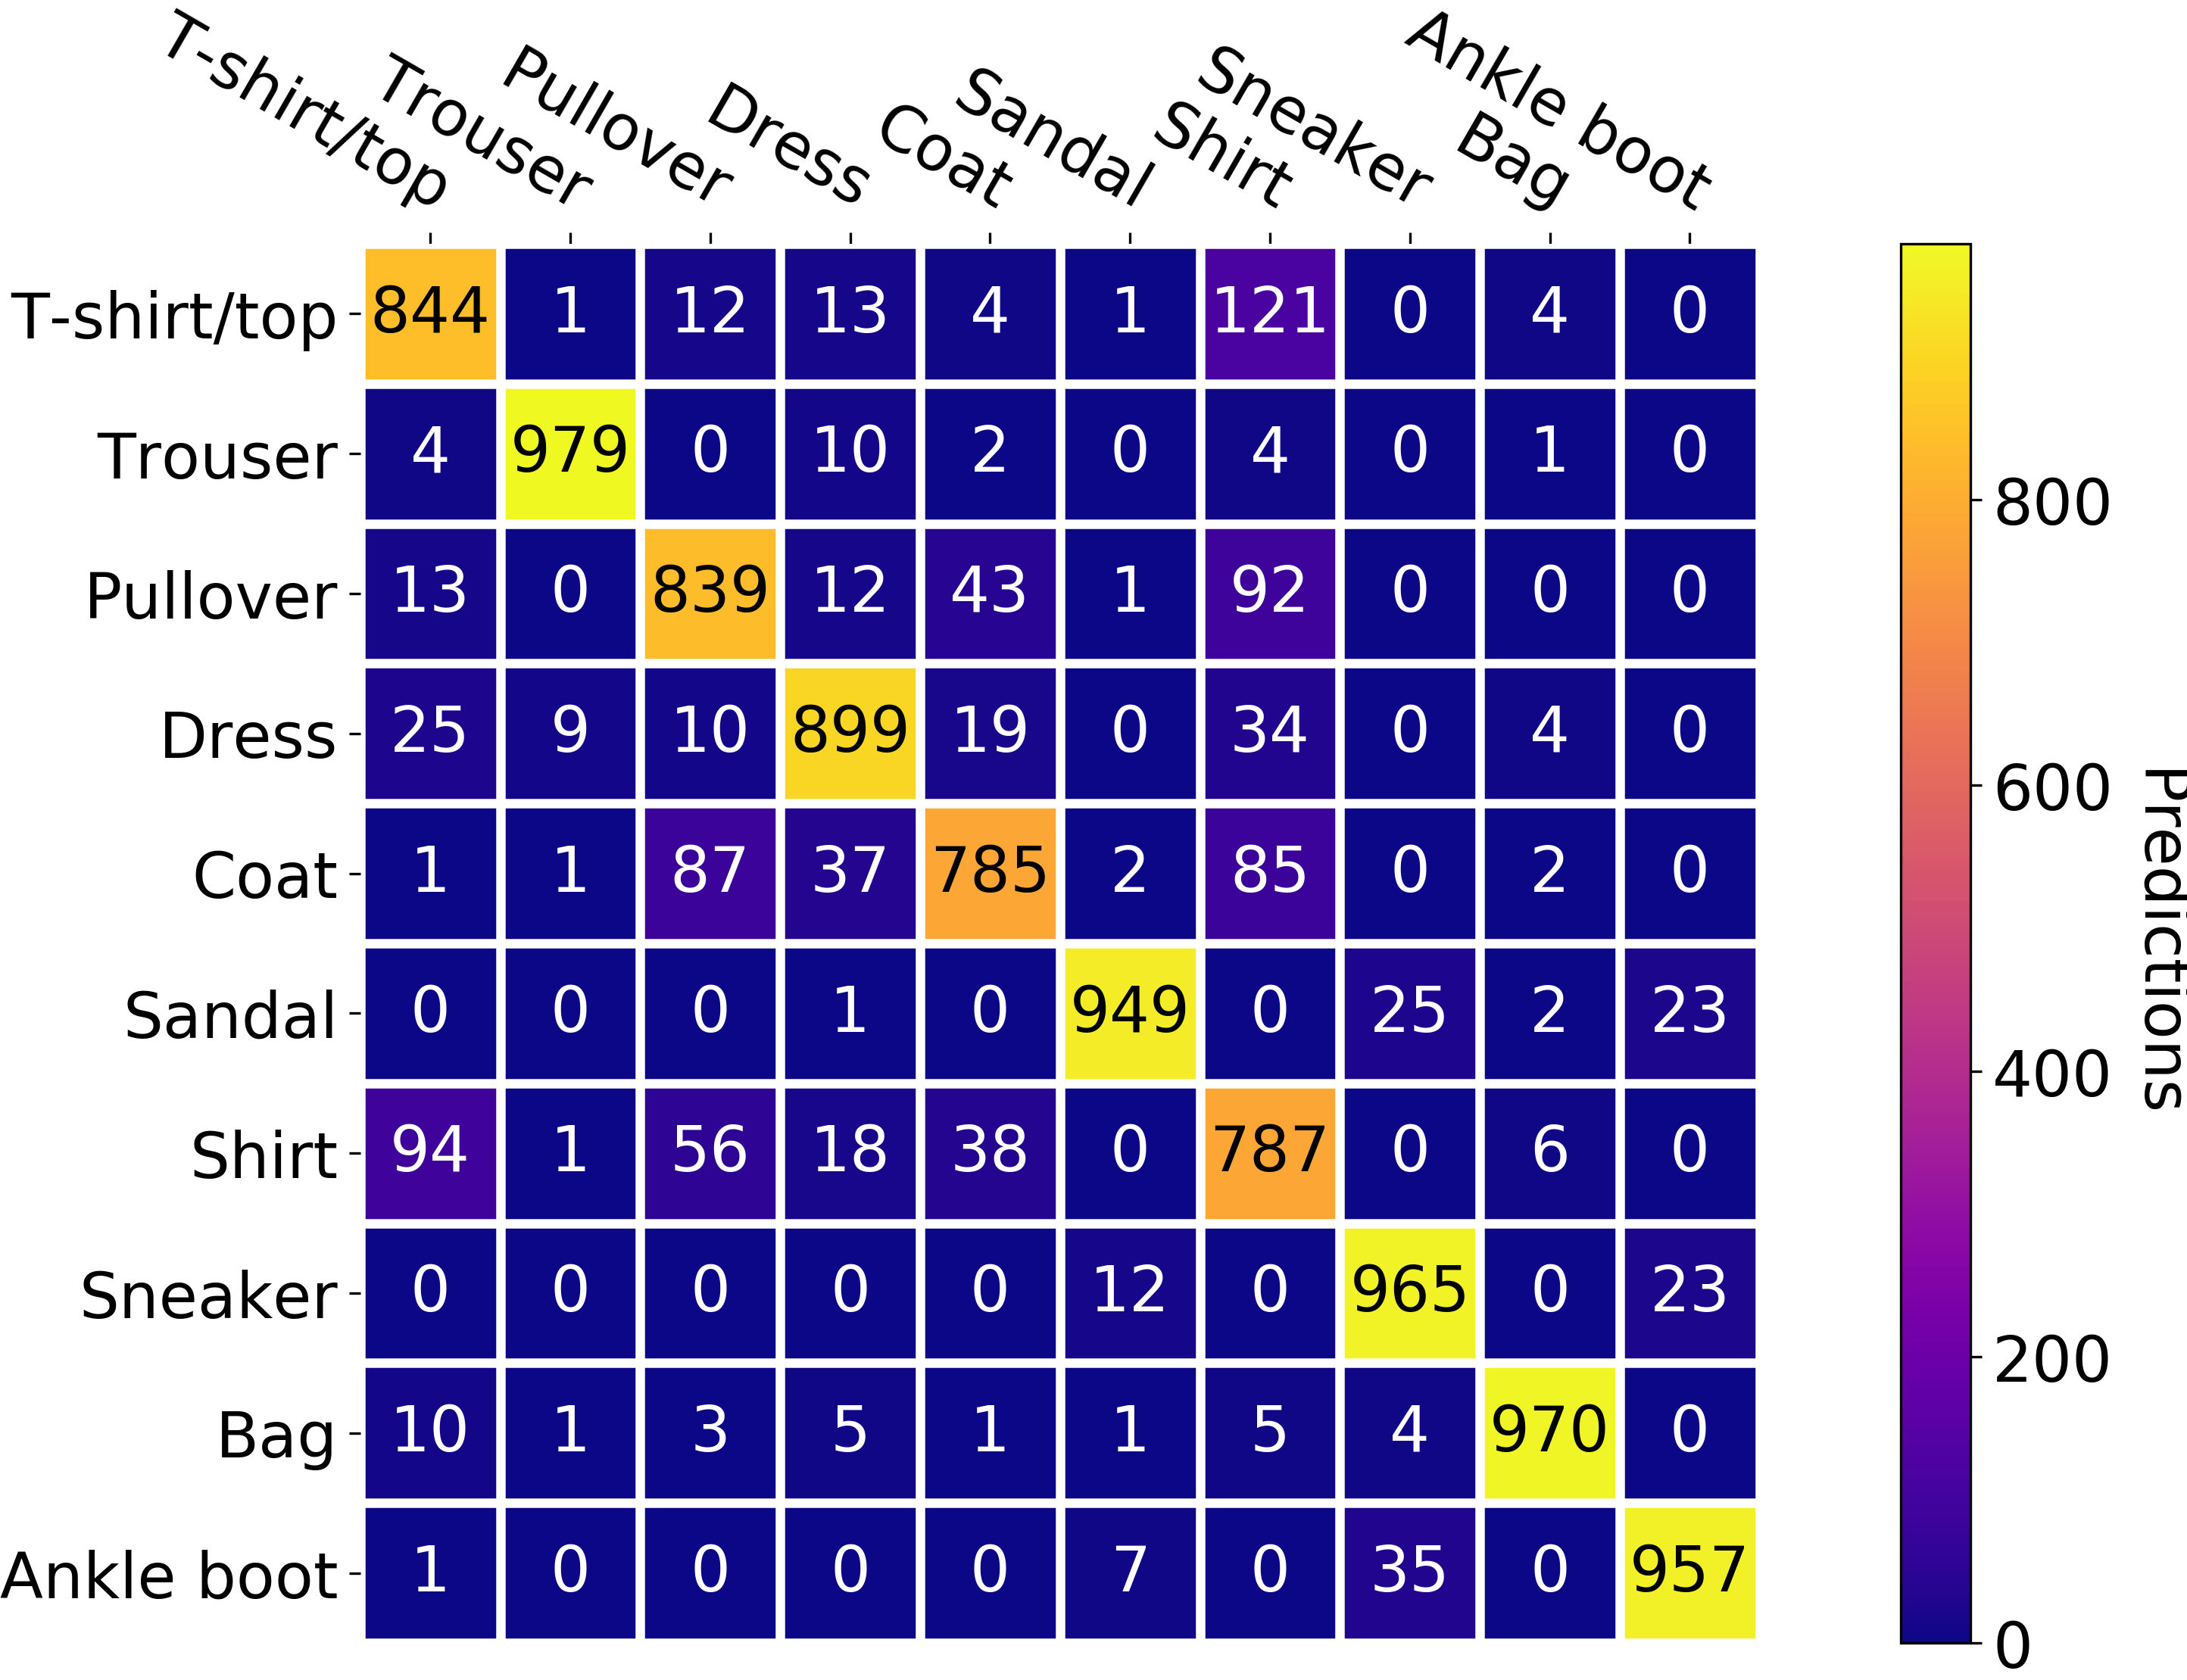
\includegraphics[width=\linewidth]{task_1_cm.png}
  \caption{FCNN Confusion Matrix as a heatmap. Brighter diagonal means the NN did better. Any cell off
   the diagonal that is bright represents severe misclassification. Rows are predictions, columns are ground truth.}
  \label{fig:task_1_cm}
\end{figure}

\begin{table}[]
  \centering
  \caption{Accuracy across optimizers on FCNN.}
  \label{tab:FCNN}
  \begin{tabular}{|c|c|c|c|c|c|c|c|}
  \hline
   & SGD & RMSprop & Adagrad & Adadelta & Adam & Adamax & Nadam \\ \hline
   Categorical C.E. & 84.64\% & 89.63\% & 80.95\% & 74.04\% & 88.65\% & \textbf{89.74\%} & 89.28\% \\ \hline
  \end{tabular}
  \end{table}


\subsection{Small Convolutional Neural Network}

In Figures \ref{fig:task_2_loss_epochs}, \ref{fig:task_2_loss_time}, and \ref{fig:task_2_acc_epochs}, we can see
 the loss and accuracy during training.
Similar to the FCNN, three of the optimizers seem to get a slow start and never manage to catch back up to the other four.
The networks using the other four optimizers also started to experience overfitting early in training.
This can be better seen in Figure \ref{fig:task_2_acc_epochs}.

In Figure \ref{fig:task_2_cm}, we can see that the SCNN did better than the FCNN
 at discerning between similar clothing types, but still somewhat poorly on similar clothes.
Shirts were still especially challenging, but t-shirts and coats were less of a challenge than they were for the FCNN.

In Table \ref{tab:SCNN} we can see the final results of our experiments on the SCNN.
Overall, most performed in the upper 80s, lower 90s range which is pretty good.
Adadelta was the worst by a mile at 78.17\%.
Adamax barely managed to get the best performance with 91.93\%.

\begin{figure}
  \centering
  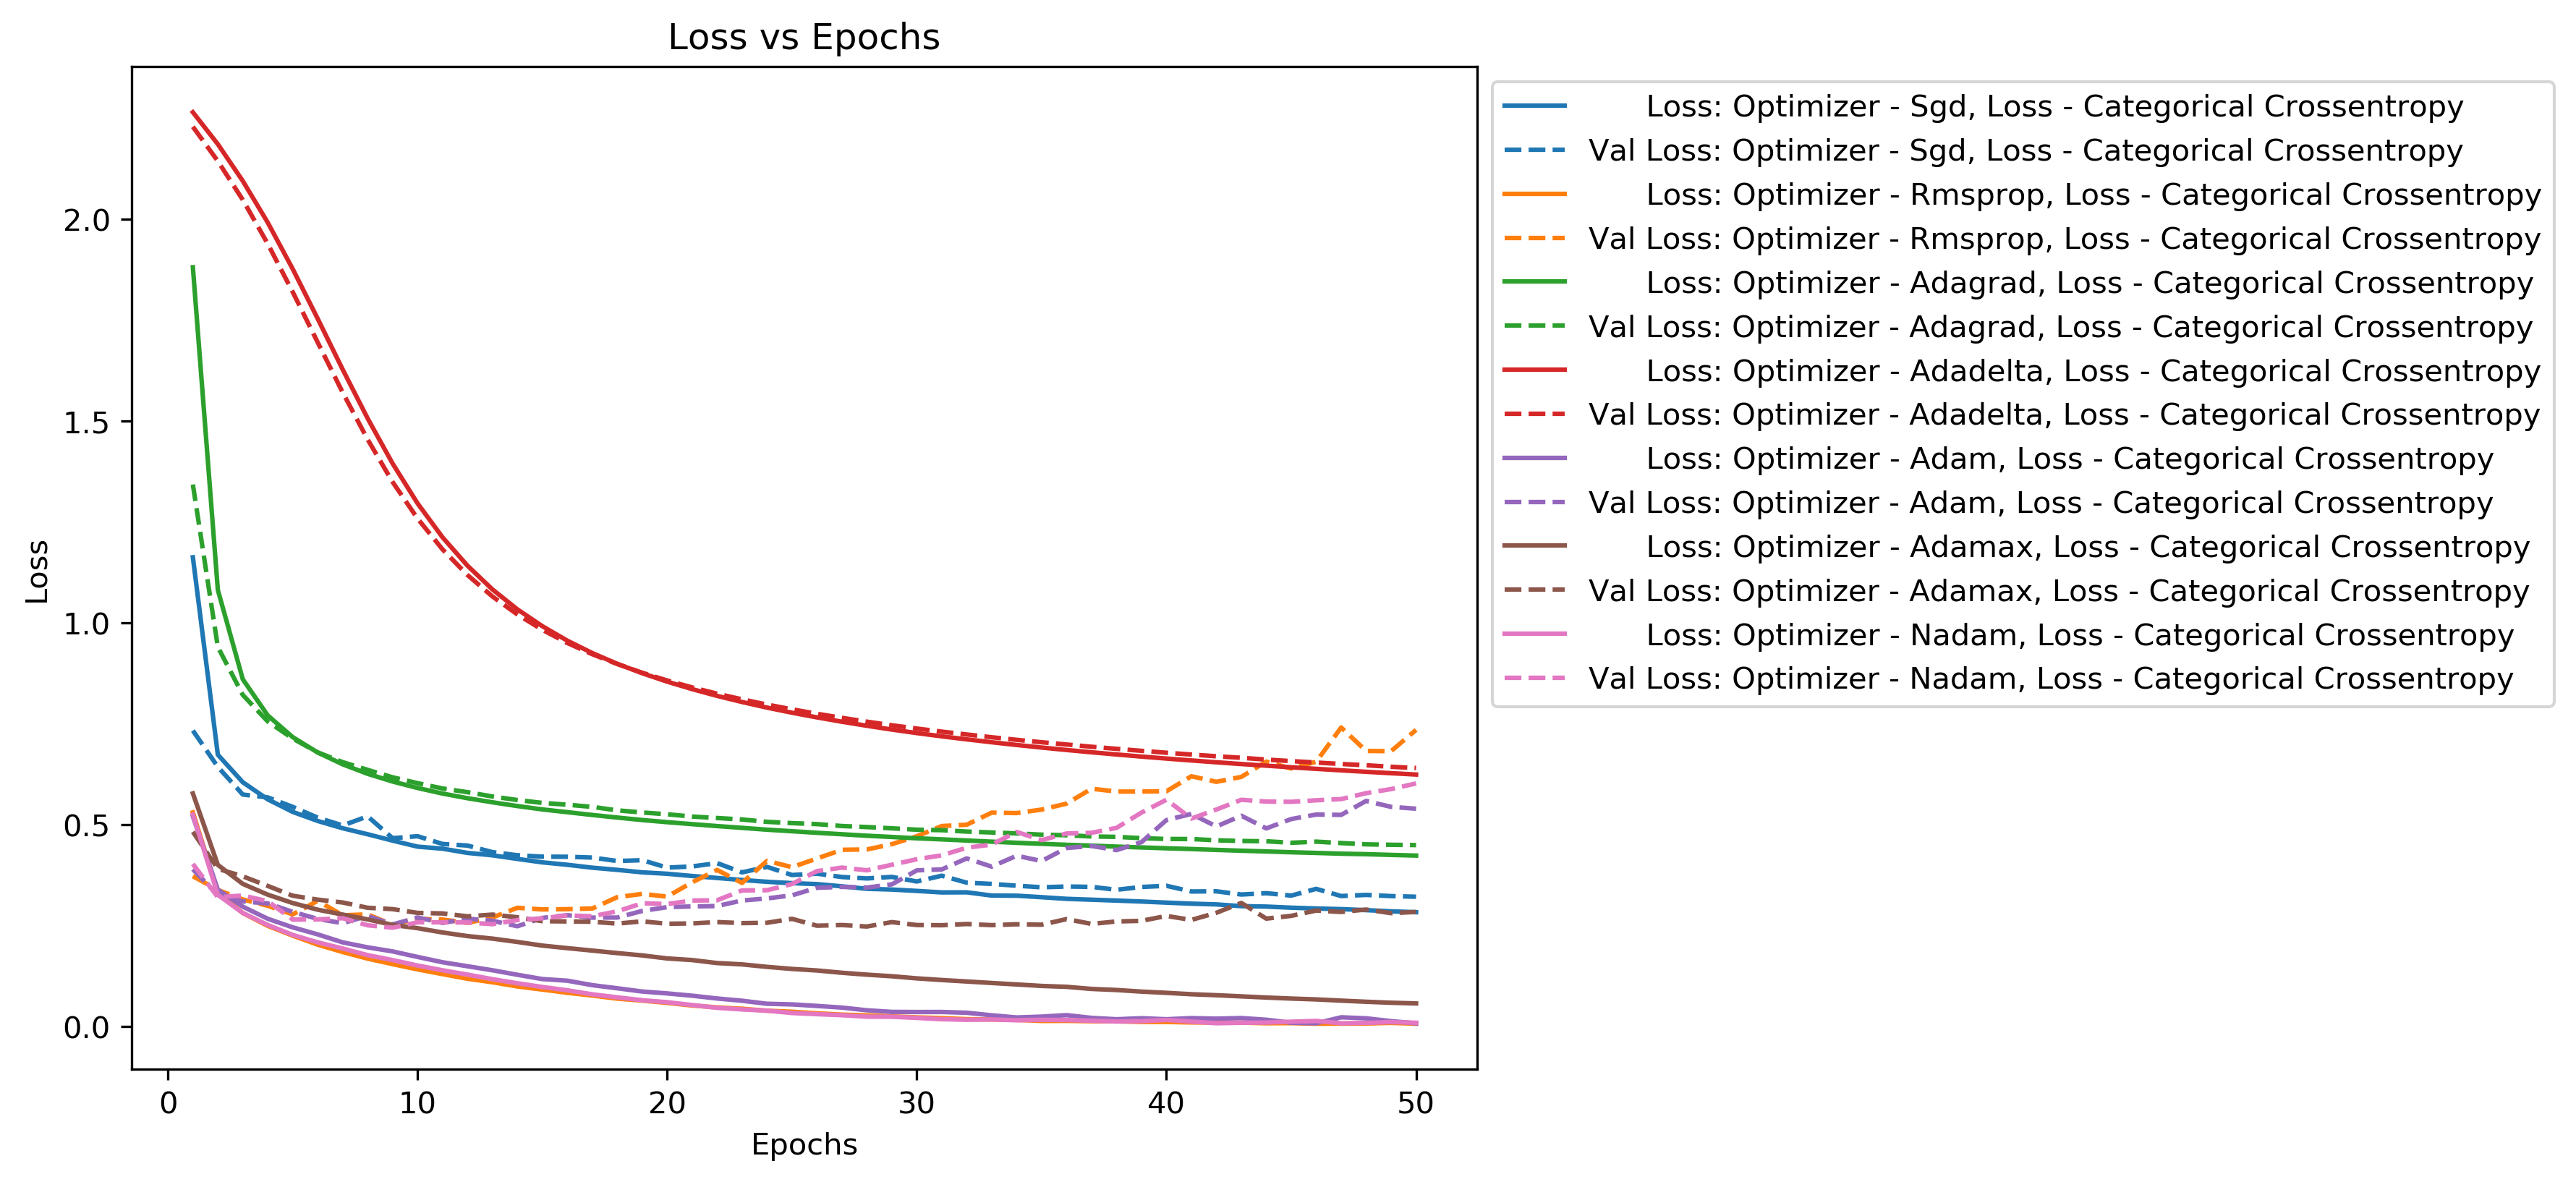
\includegraphics[width=\linewidth]{task_2_loss_epochs.png}
  \caption{Loss of SCNN using different optimizers over epochs.}
  \label{fig:task_2_loss_epochs}
\end{figure}

\begin{figure}
  \centering
  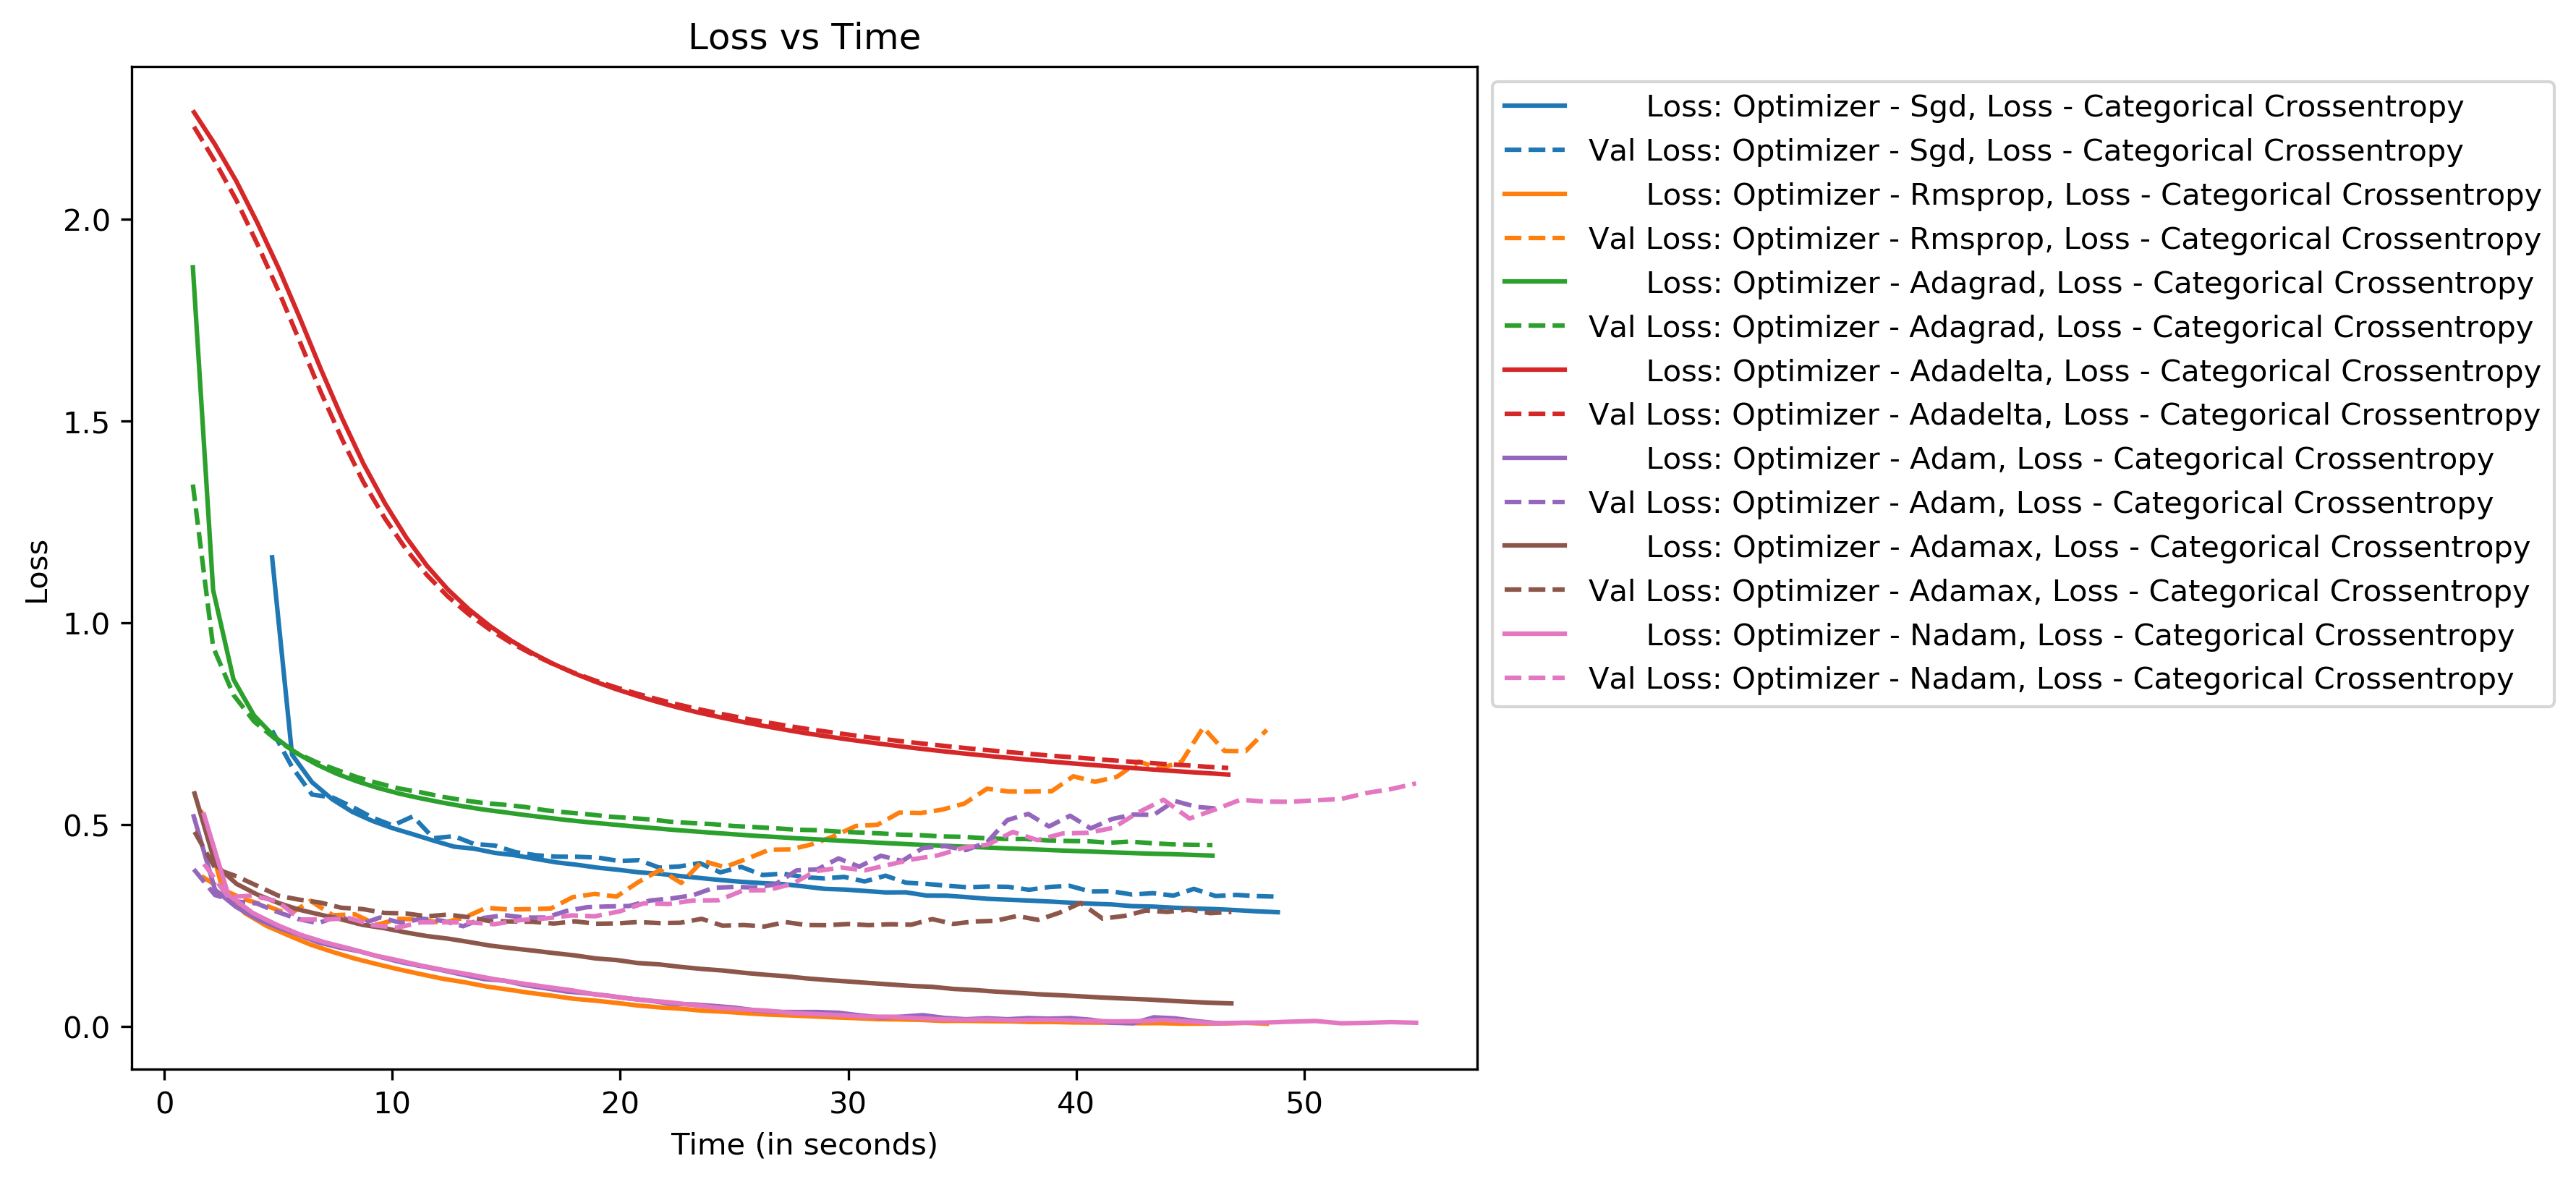
\includegraphics[width=\linewidth]{task_2_loss_time.png}
  \caption{Loss of SCNN using different optimizers over time.}
  \label{fig:task_2_loss_time}
\end{figure}

\begin{figure}
  \centering
  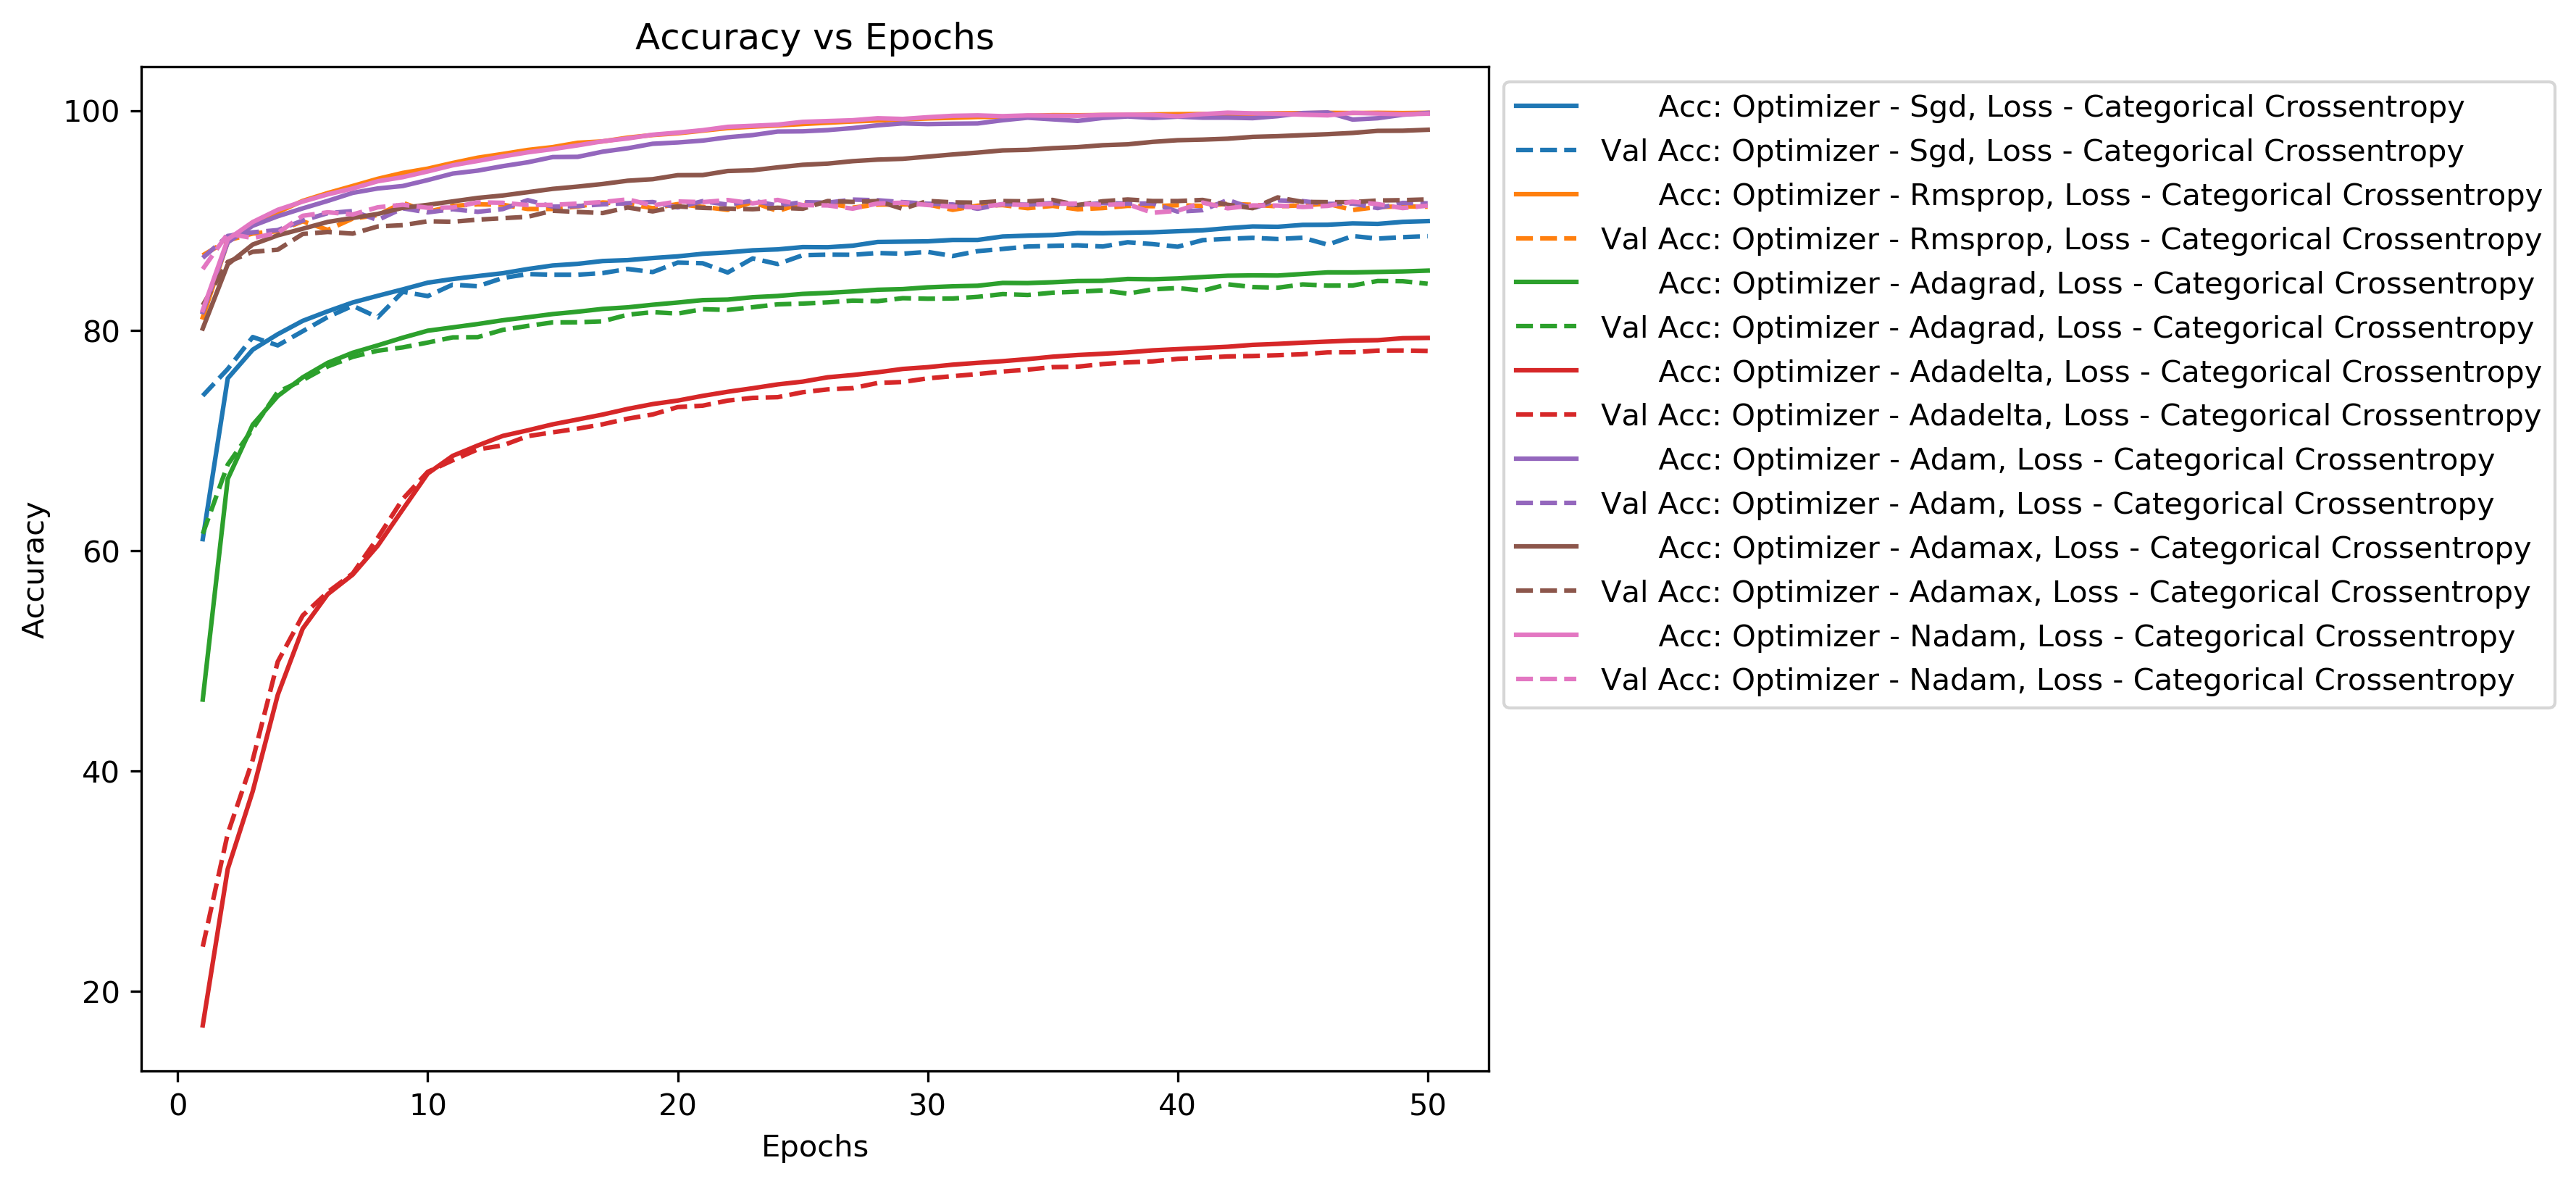
\includegraphics[width=\linewidth]{task_2_acc_epochs.png}
  \caption{Accuracy of SCNN using different optimizers over time.}
  \label{fig:task_2_acc_epochs}
\end{figure}

\begin{figure}
  \centering
  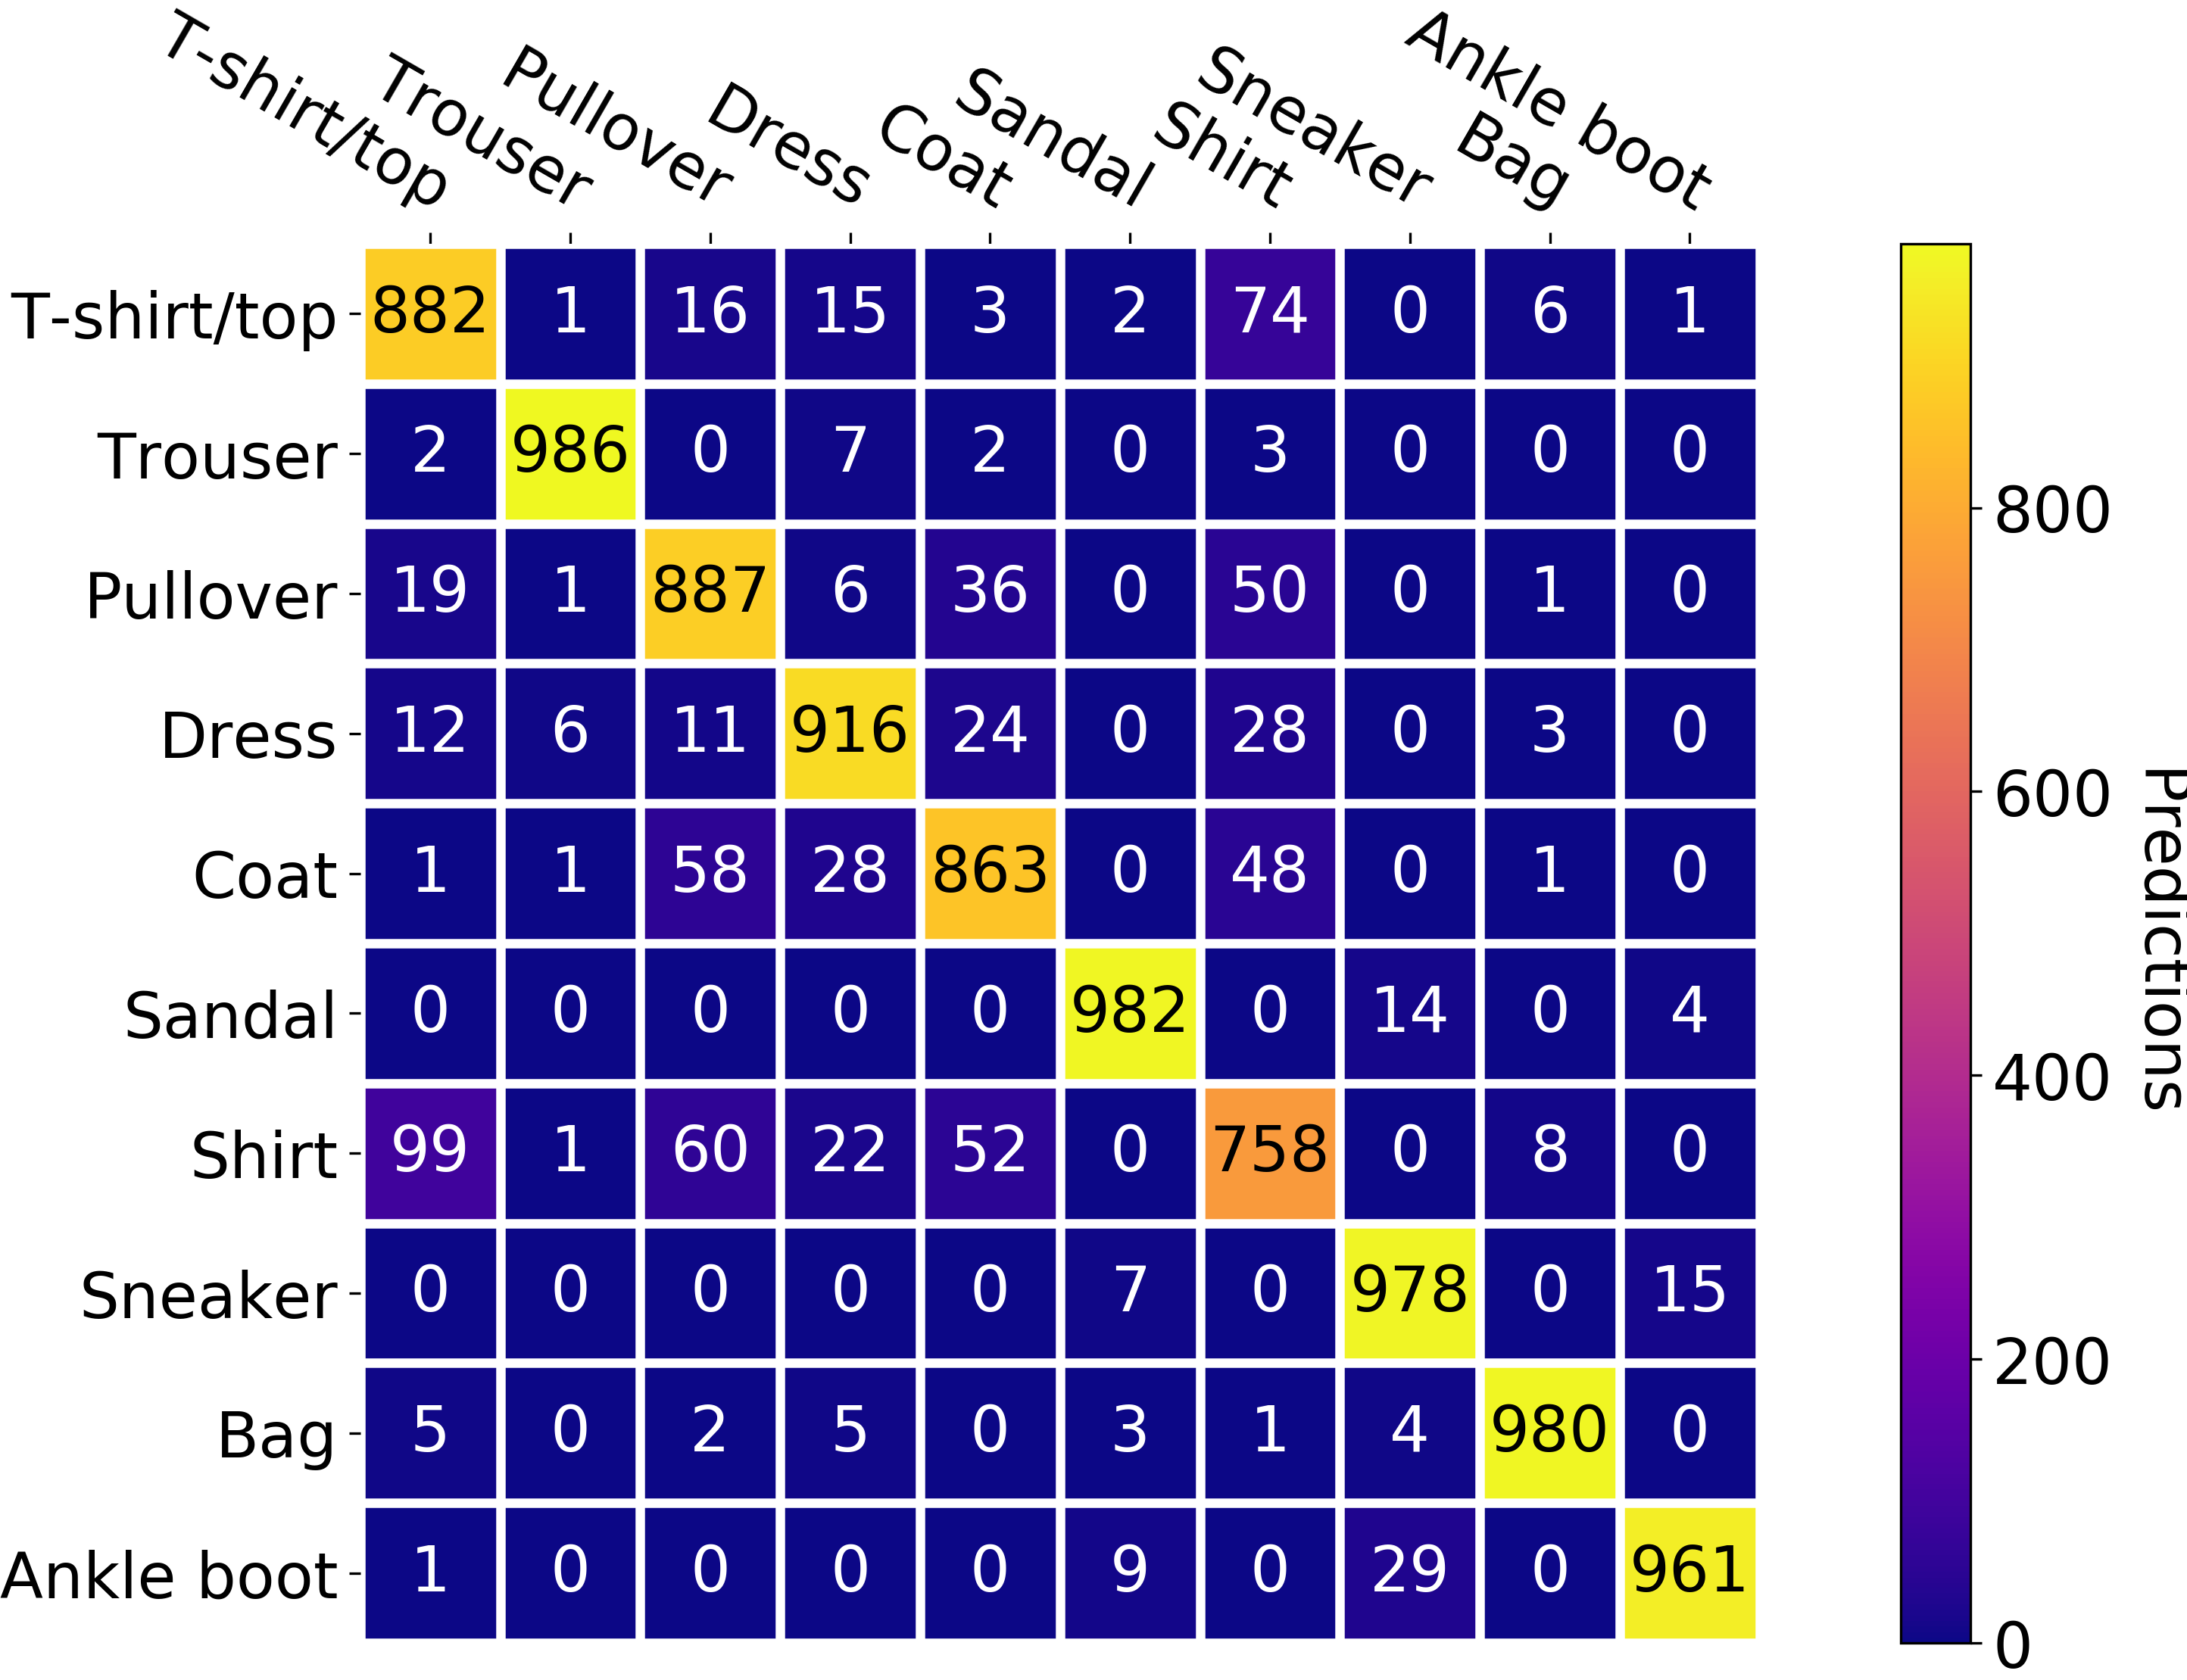
\includegraphics[width=\linewidth]{task_2_cm.png}
  \caption{SCNN Confusion Matrix as a heatmap. Brighter diagonal means the NN did better. Any cell off
   the diagonal that is bright represents severe misclassification. Rows are predictions, columns are ground truth.}
  \label{fig:task_2_cm}
\end{figure}

\begin{table}[]
  \centering
  \caption{Accuracy across optimizers on SCNN.}
  \label{tab:SCNN}
  \begin{tabular}{|c|c|c|c|c|c|c|c|}
  \hline
   & SGD & RMSprop & Adagrad & Adadelta & Adam & Adamax & Nadam \\ \hline
   Categorical C.E. & 88.59\% & 91.27\% & 84.27\% & 78.17\% & 91.57\% & \textbf{91.93\%} & 91.36\% \\ \hline
  \end{tabular}
  \end{table}


\subsection{Bigger Convolutional Neural Network}

In Figures \ref{fig:task_3_loss_epochs}, \ref{fig:task_3_loss_time}, and \ref{fig:task_3_acc_epochs}, we can see
 the loss and accuracy during training.
Similar to the FCNN and SCNN, three of the optimizers get a slow start and never manage to catch back up to the other four.
The networks using the other four optimizers also started to experience overfitting early on in training.
This can be better seen in Figure \ref{fig:task_3_acc_epochs}.

In Figure \ref{fig:task_3_cm}, we can see that the BCNN did better than the FCNN
 at discerning between similar clothing types, but still somewhat poorly on similar clothes.
It was comparable in performance to the SCNN, and they both had similar strengths and weaknesses according to their confusion matrices.

In Table \ref{tab:BCNN} we can see the final results of our experiments on the BCNN.
Overall, most performed in the lower 90s range which is starting to be really good.
Adadelta performed the worst at an atrocious 73.24\%.
This time Adam won with the best performance at 91.86\%.
BCNN mostly performed on par with SCNN, potentially showing that the extra filters were not needed and might cause more problems than the ones they solve.

\begin{figure}
  \centering
  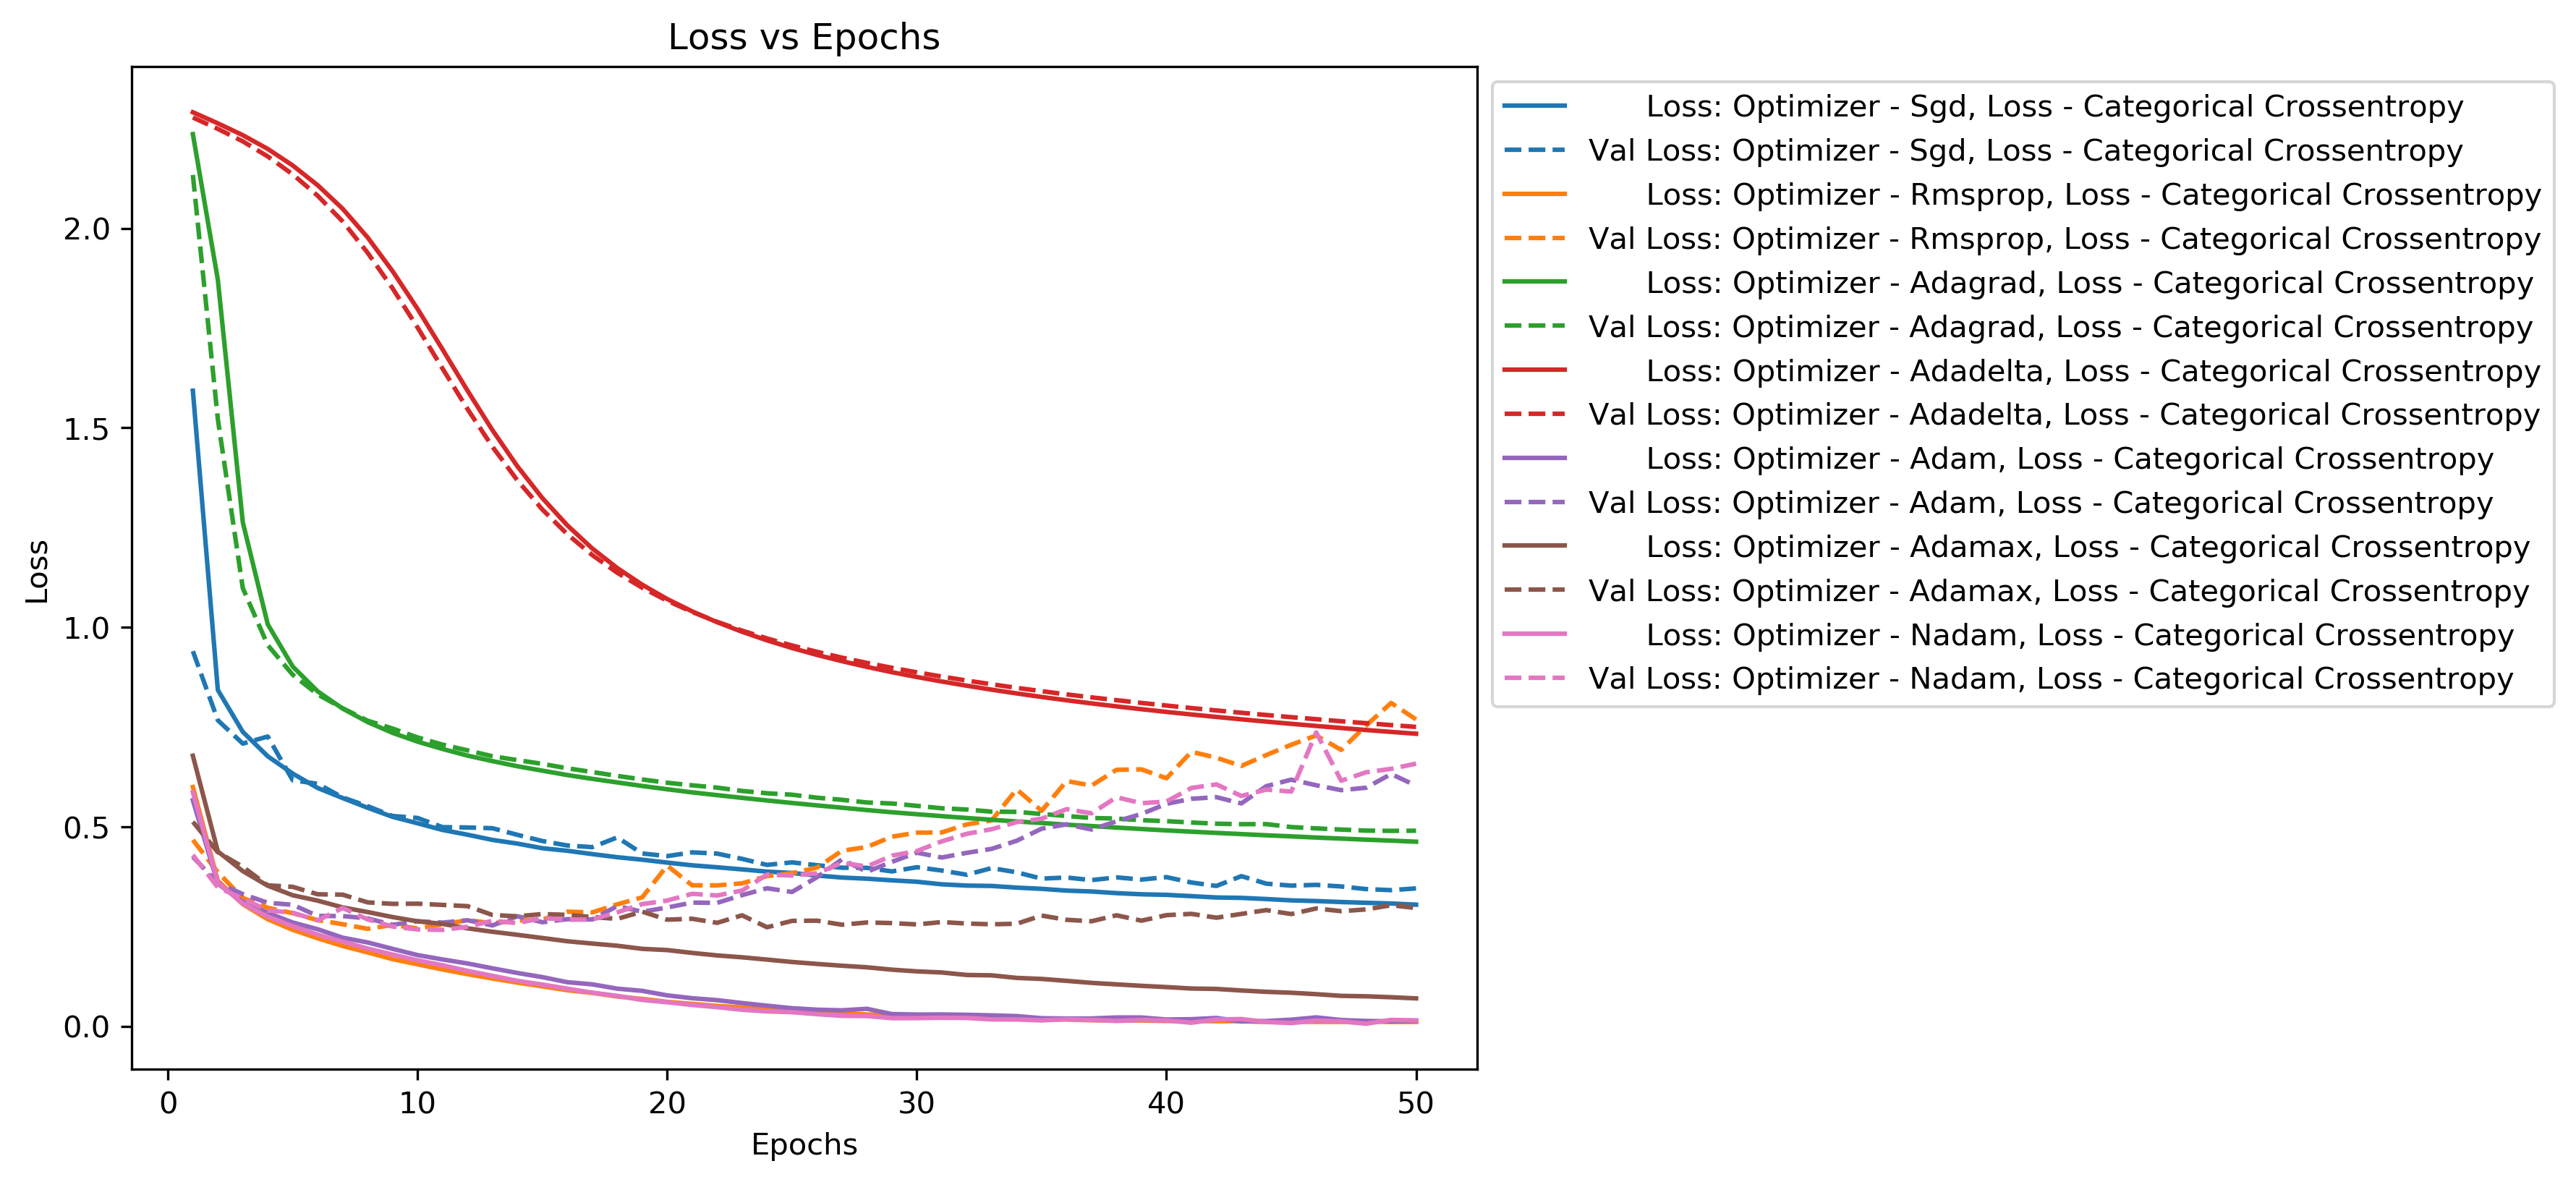
\includegraphics[width=\linewidth]{task_3_loss_epochs.png}
  \caption{Loss of BCNN using different optimizers over epochs.}
  \label{fig:task_3_loss_epochs}
\end{figure}

\begin{figure}
  \centering
  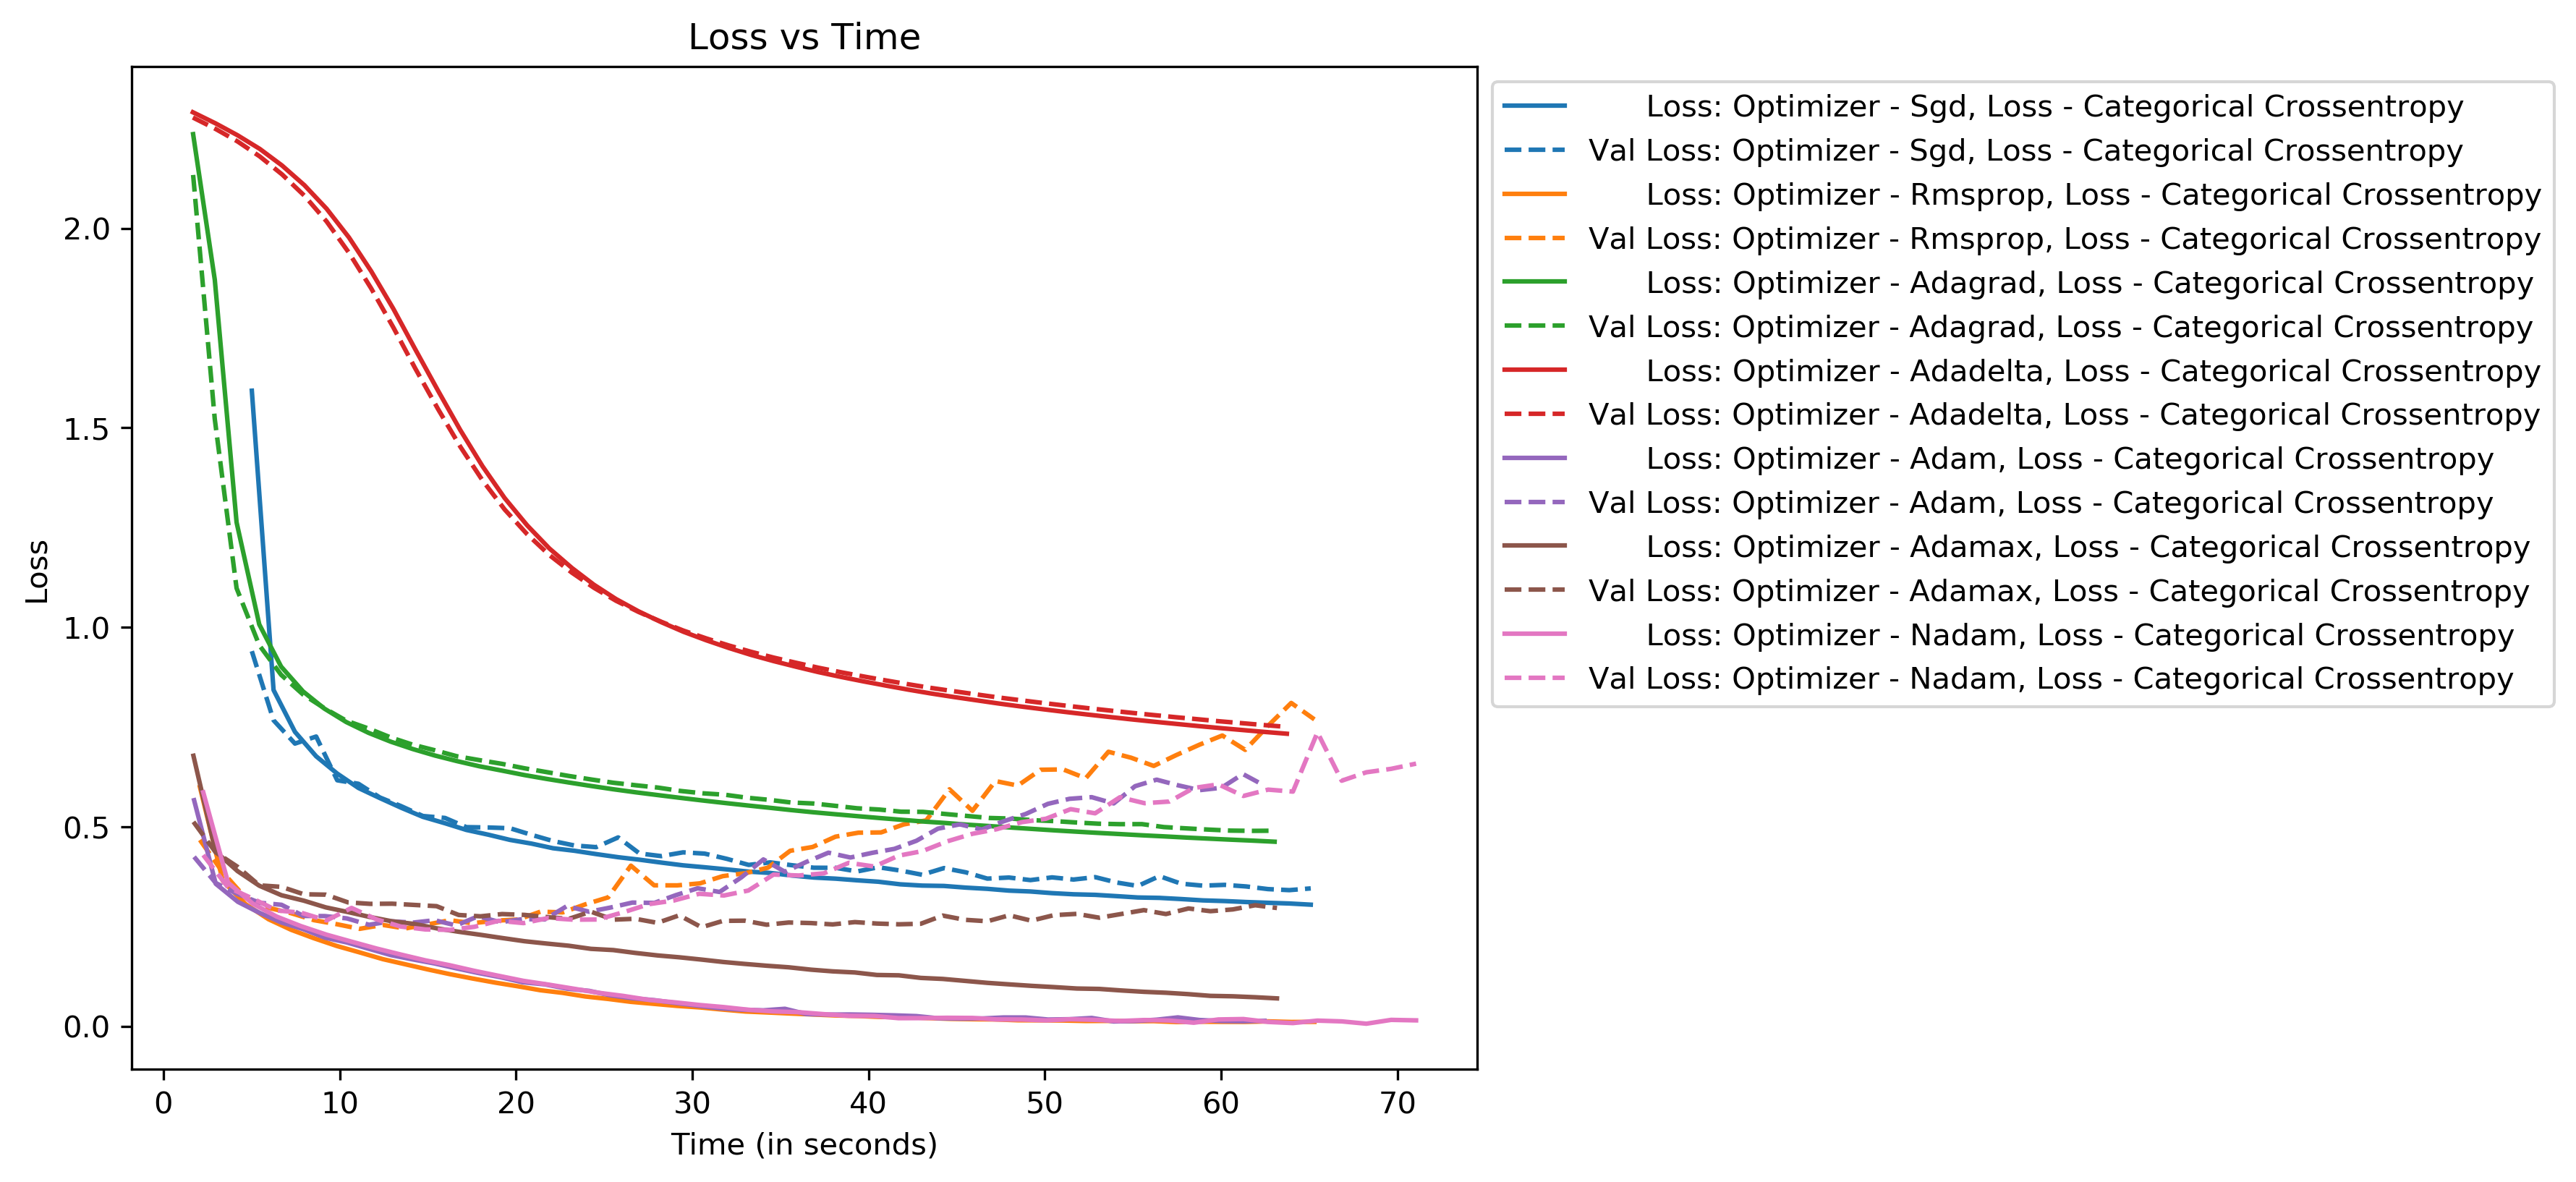
\includegraphics[width=\linewidth]{task_3_loss_time.png}
  \caption{Loss of BCNN using different optimizers over time.}
  \label{fig:task_3_loss_time}
\end{figure}

\begin{figure}
  \centering
  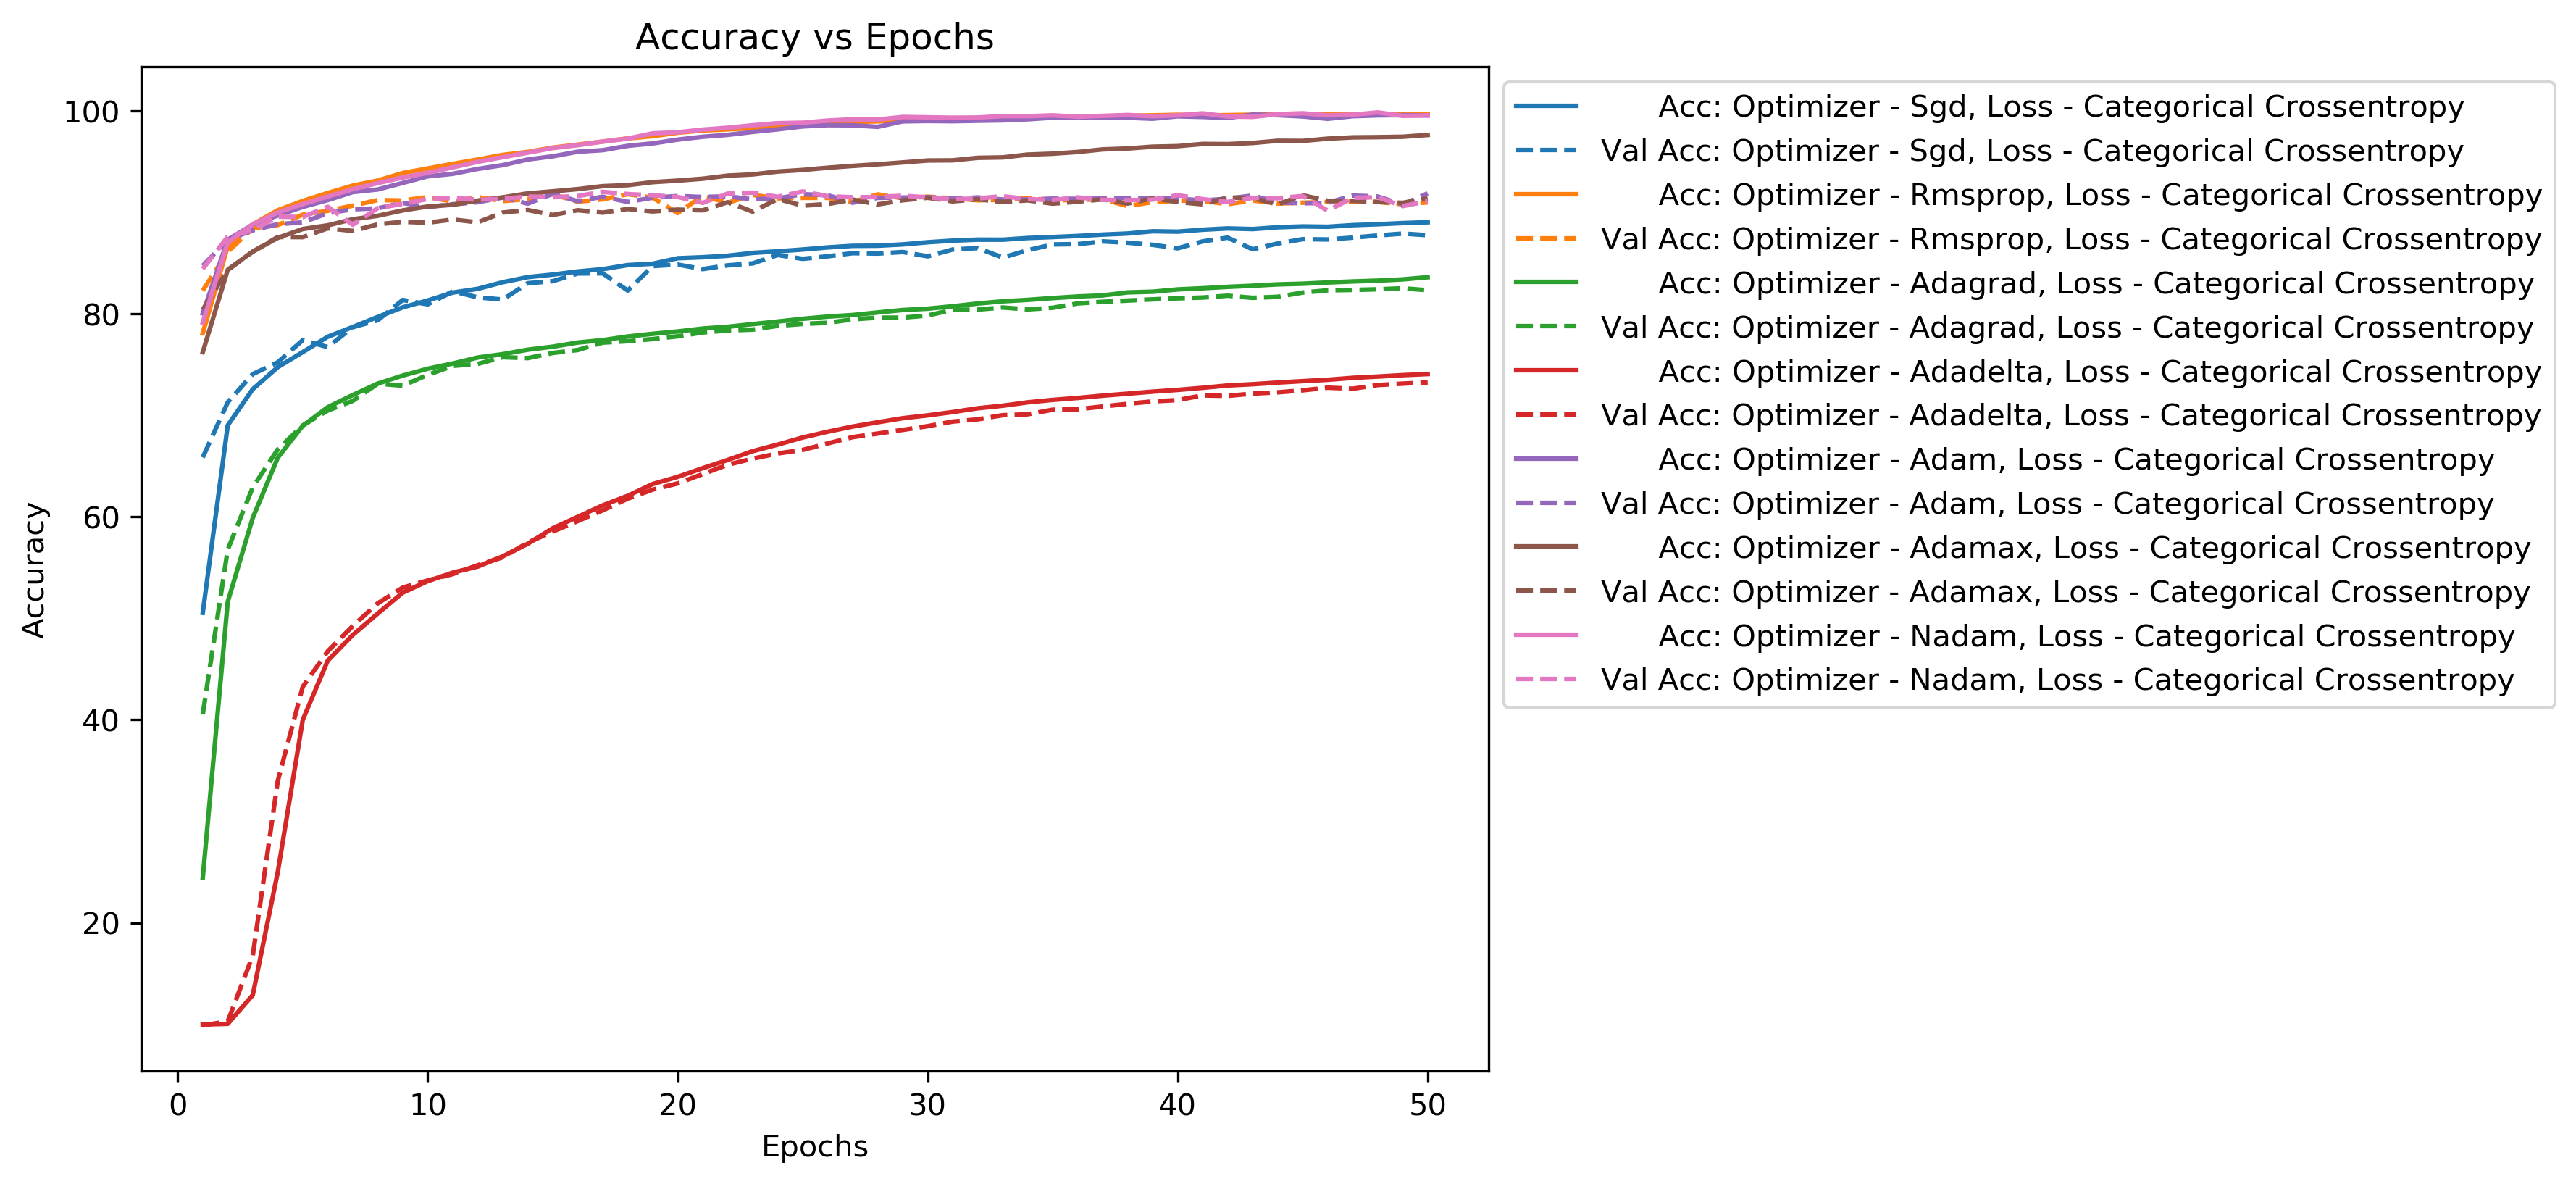
\includegraphics[width=\linewidth]{task_3_acc_epochs.png}
  \caption{Accuracy of BCNN using different optimizers over time.}
  \label{fig:task_3_acc_epochs}
\end{figure}

\begin{figure}
  \centering
  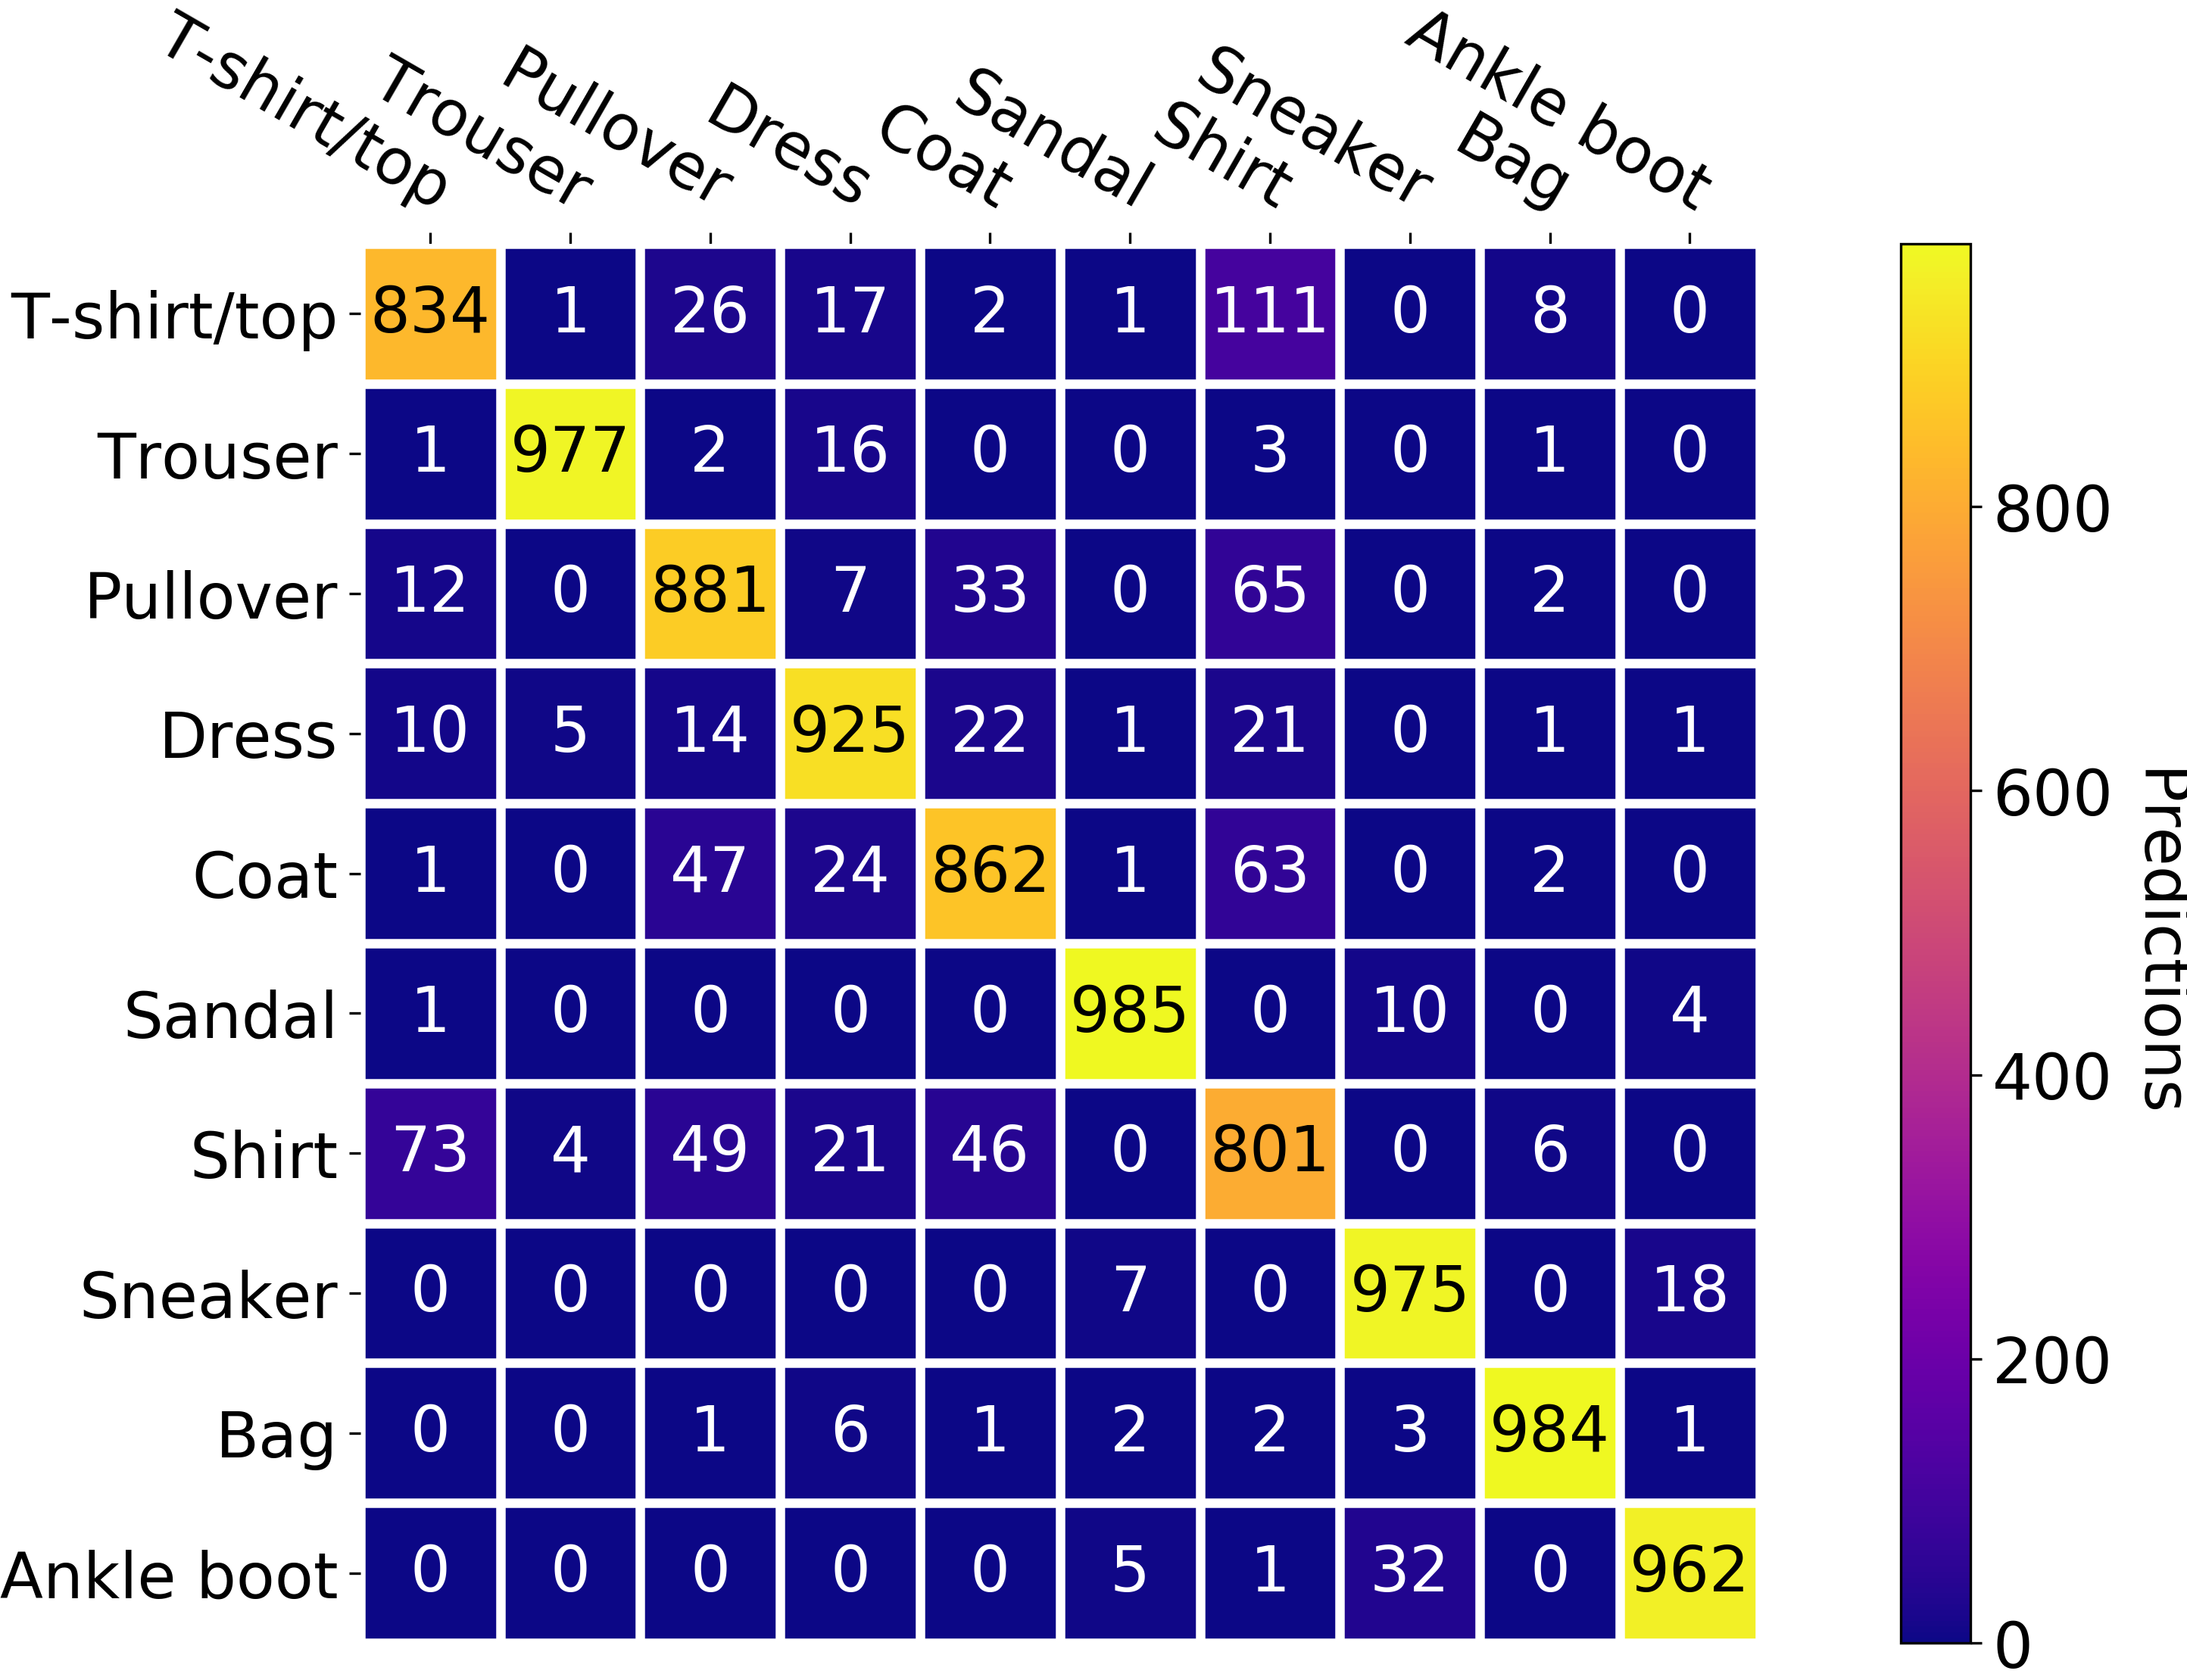
\includegraphics[width=\linewidth]{task_3_cm.png}
  \caption{BCNN Confusion Matrix as a heatmap. Brighter diagonal means the NN did better. Any cell off
   the diagonal that is bright represents severe misclassification. Rows are predictions, columns are ground truth.}
  \label{fig:task_3_cm}
\end{figure}

\begin{table}[]
  \centering
  \caption{Accuracy across optimizers on BCNN.}
  \label{tab:BCNN}
  \begin{tabular}{|c|c|c|c|c|c|c|c|}
  \hline
   & SGD & RMSprop & Adagrad & Adadelta & Adam & Adamax & Nadam \\ \hline
  Categorical C.E. & 87.74\% & 90.97\% & 82.32\% & 73.24\% & \textbf{91.86\%} & 91.36\% & 91.09\% \\ \hline
  \end{tabular}
  \end{table}


\subsection{My Convolutional Neural Network}

In Figures \ref{fig:task_4_loss_epochs}, \ref{fig:task_4_loss_time}, and \ref{fig:task_4_acc_epochs}, we can see
 the loss and accuracy during training.
This time, while three of the optimizers did do worse than the other four, only one was egregiously bad, Adadelta.
SGD and Adagrad started off poorly but they managed to get close to where the other four ended up.
The networks using the other four optimizers experienced overfitting early on in training, but not quite as extremely as FCNN, SCNN, and BCNN did.
This can be better seen in Figure \ref{fig:task_4_acc_epochs}.

In Figure \ref{fig:task_4_cm}, we can see that the MCNN did considerably better than the other three
 at discerning between similar clothing types.
The only one it truly struggled at was confusing shirts for t-shirts and coats.
Other than that, it had a higher than 91\% hit-rate on everything else.

In Table \ref{tab:MCNN} we can see the final results of our experiments on the MCNN.
Overall, most performed in the lower to mid 90s range which is really good.
While Adadelta performed the worst, like it did for the other three, it was somewhat better at 81.50\%.
Similar to FCNN and SCNN, Adamax was marginally better than the rest at a cool 93.87\%.
MCNN managed to perform better than any of the other networks tested, showing that the more traditional architecture
 that includes double convolutions before pooling, dropout, and batch normalization does help in classification accuracy.

\begin{figure}
  \centering
  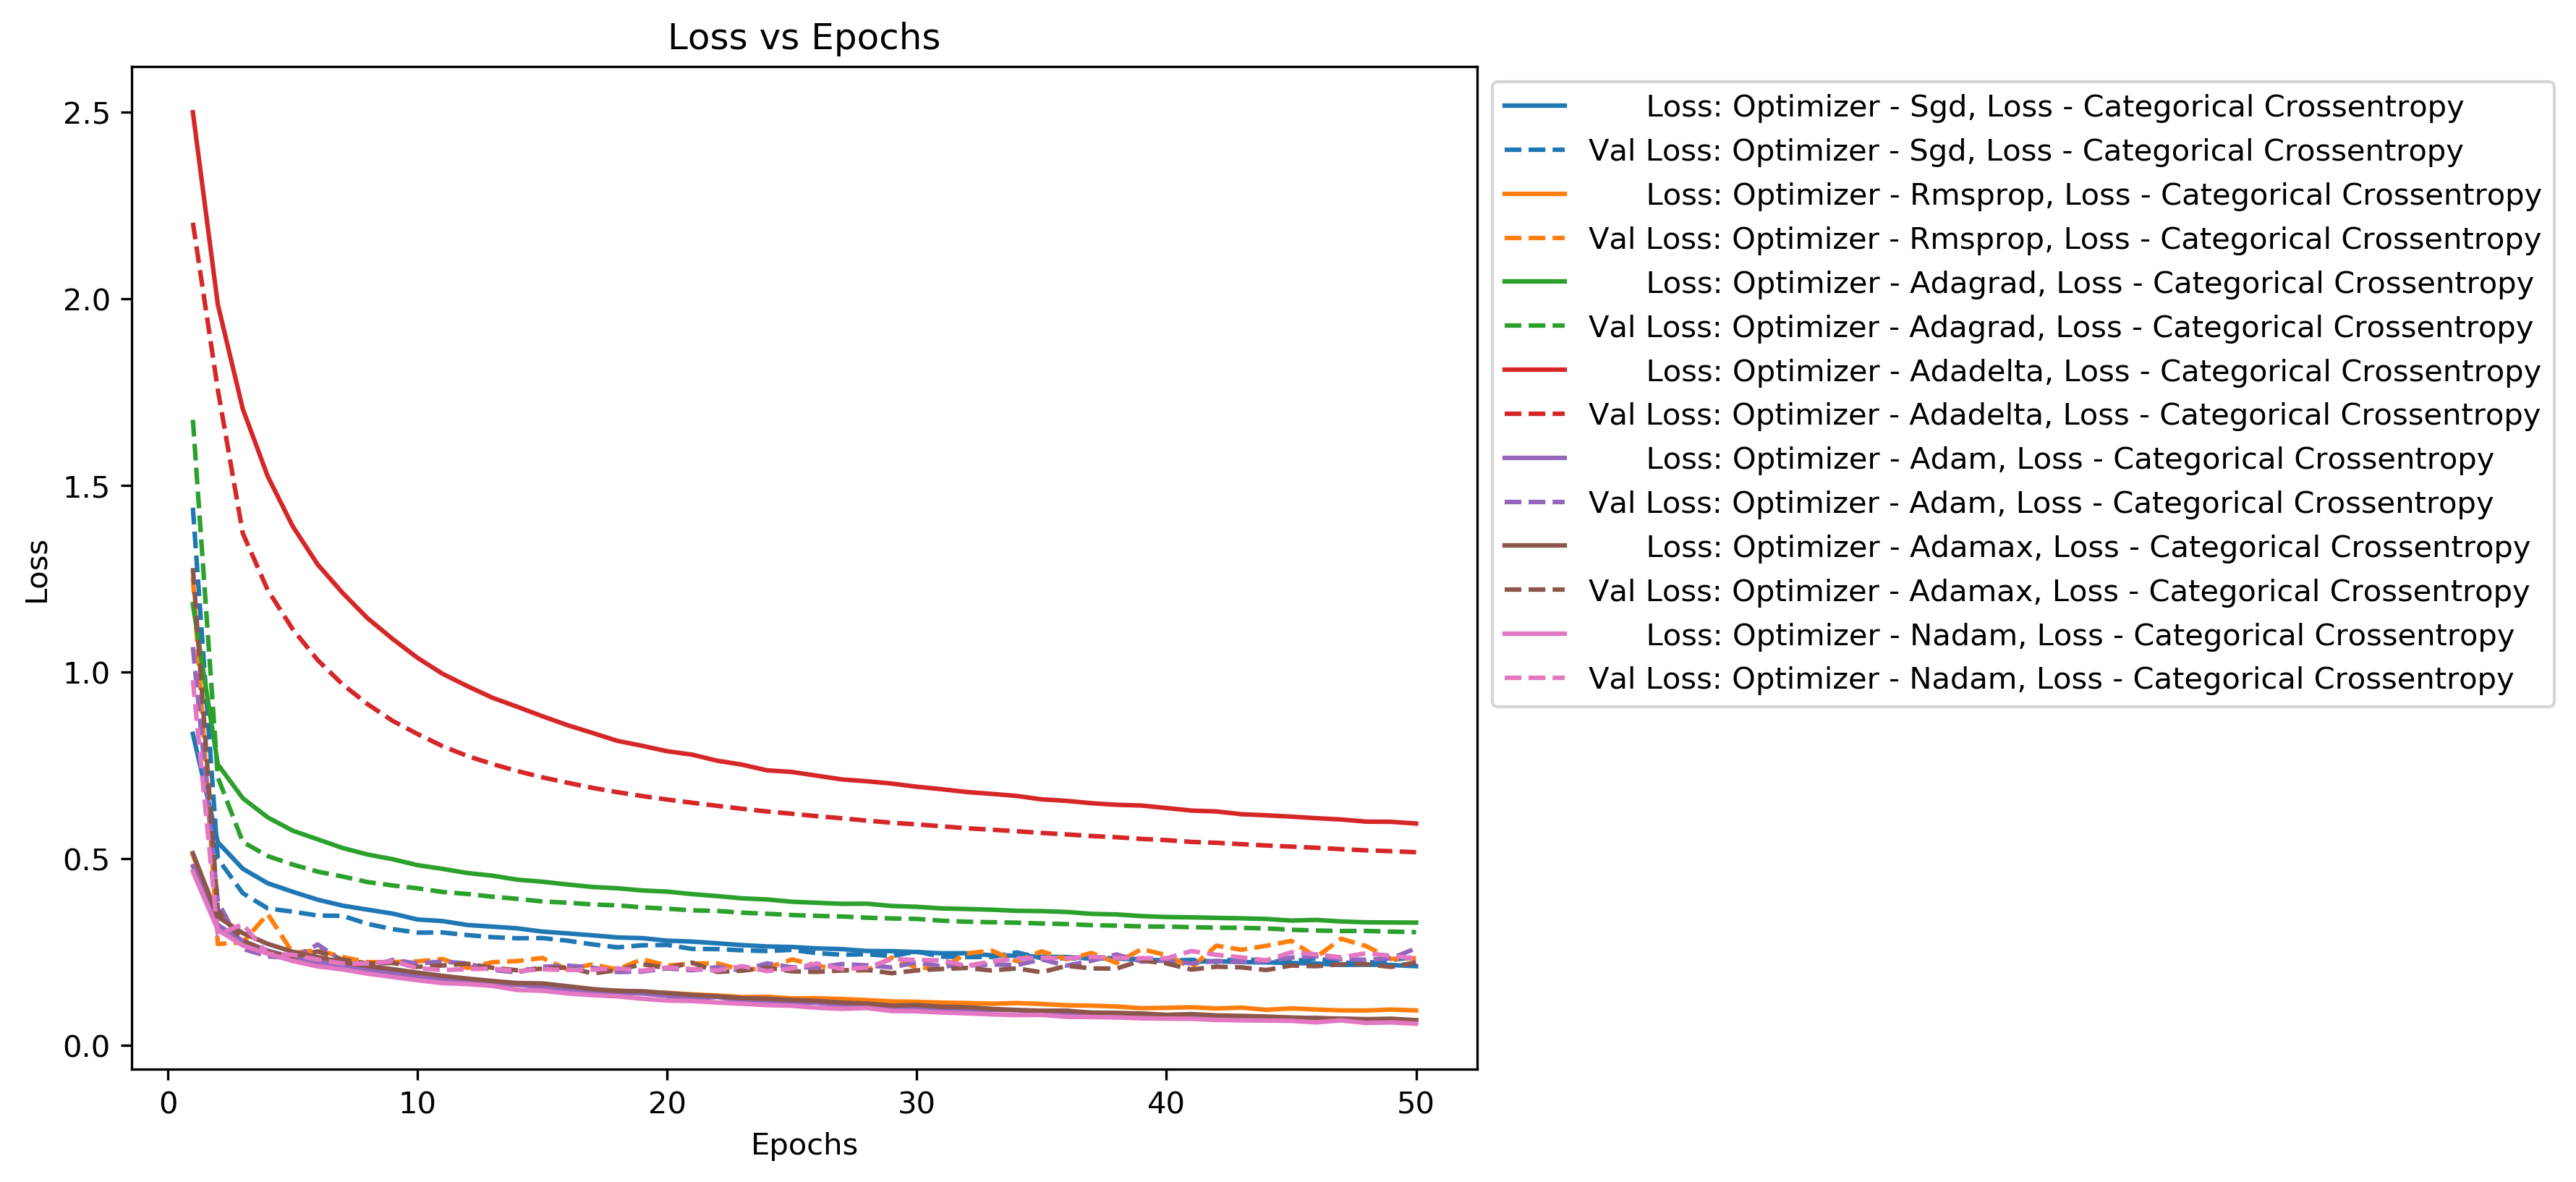
\includegraphics[width=\linewidth]{task_4_loss_epochs.png}
  \caption{Loss of MCNN using different optimizers over epochs.}
  \label{fig:task_4_loss_epochs}
\end{figure}

\begin{figure}
  \centering
  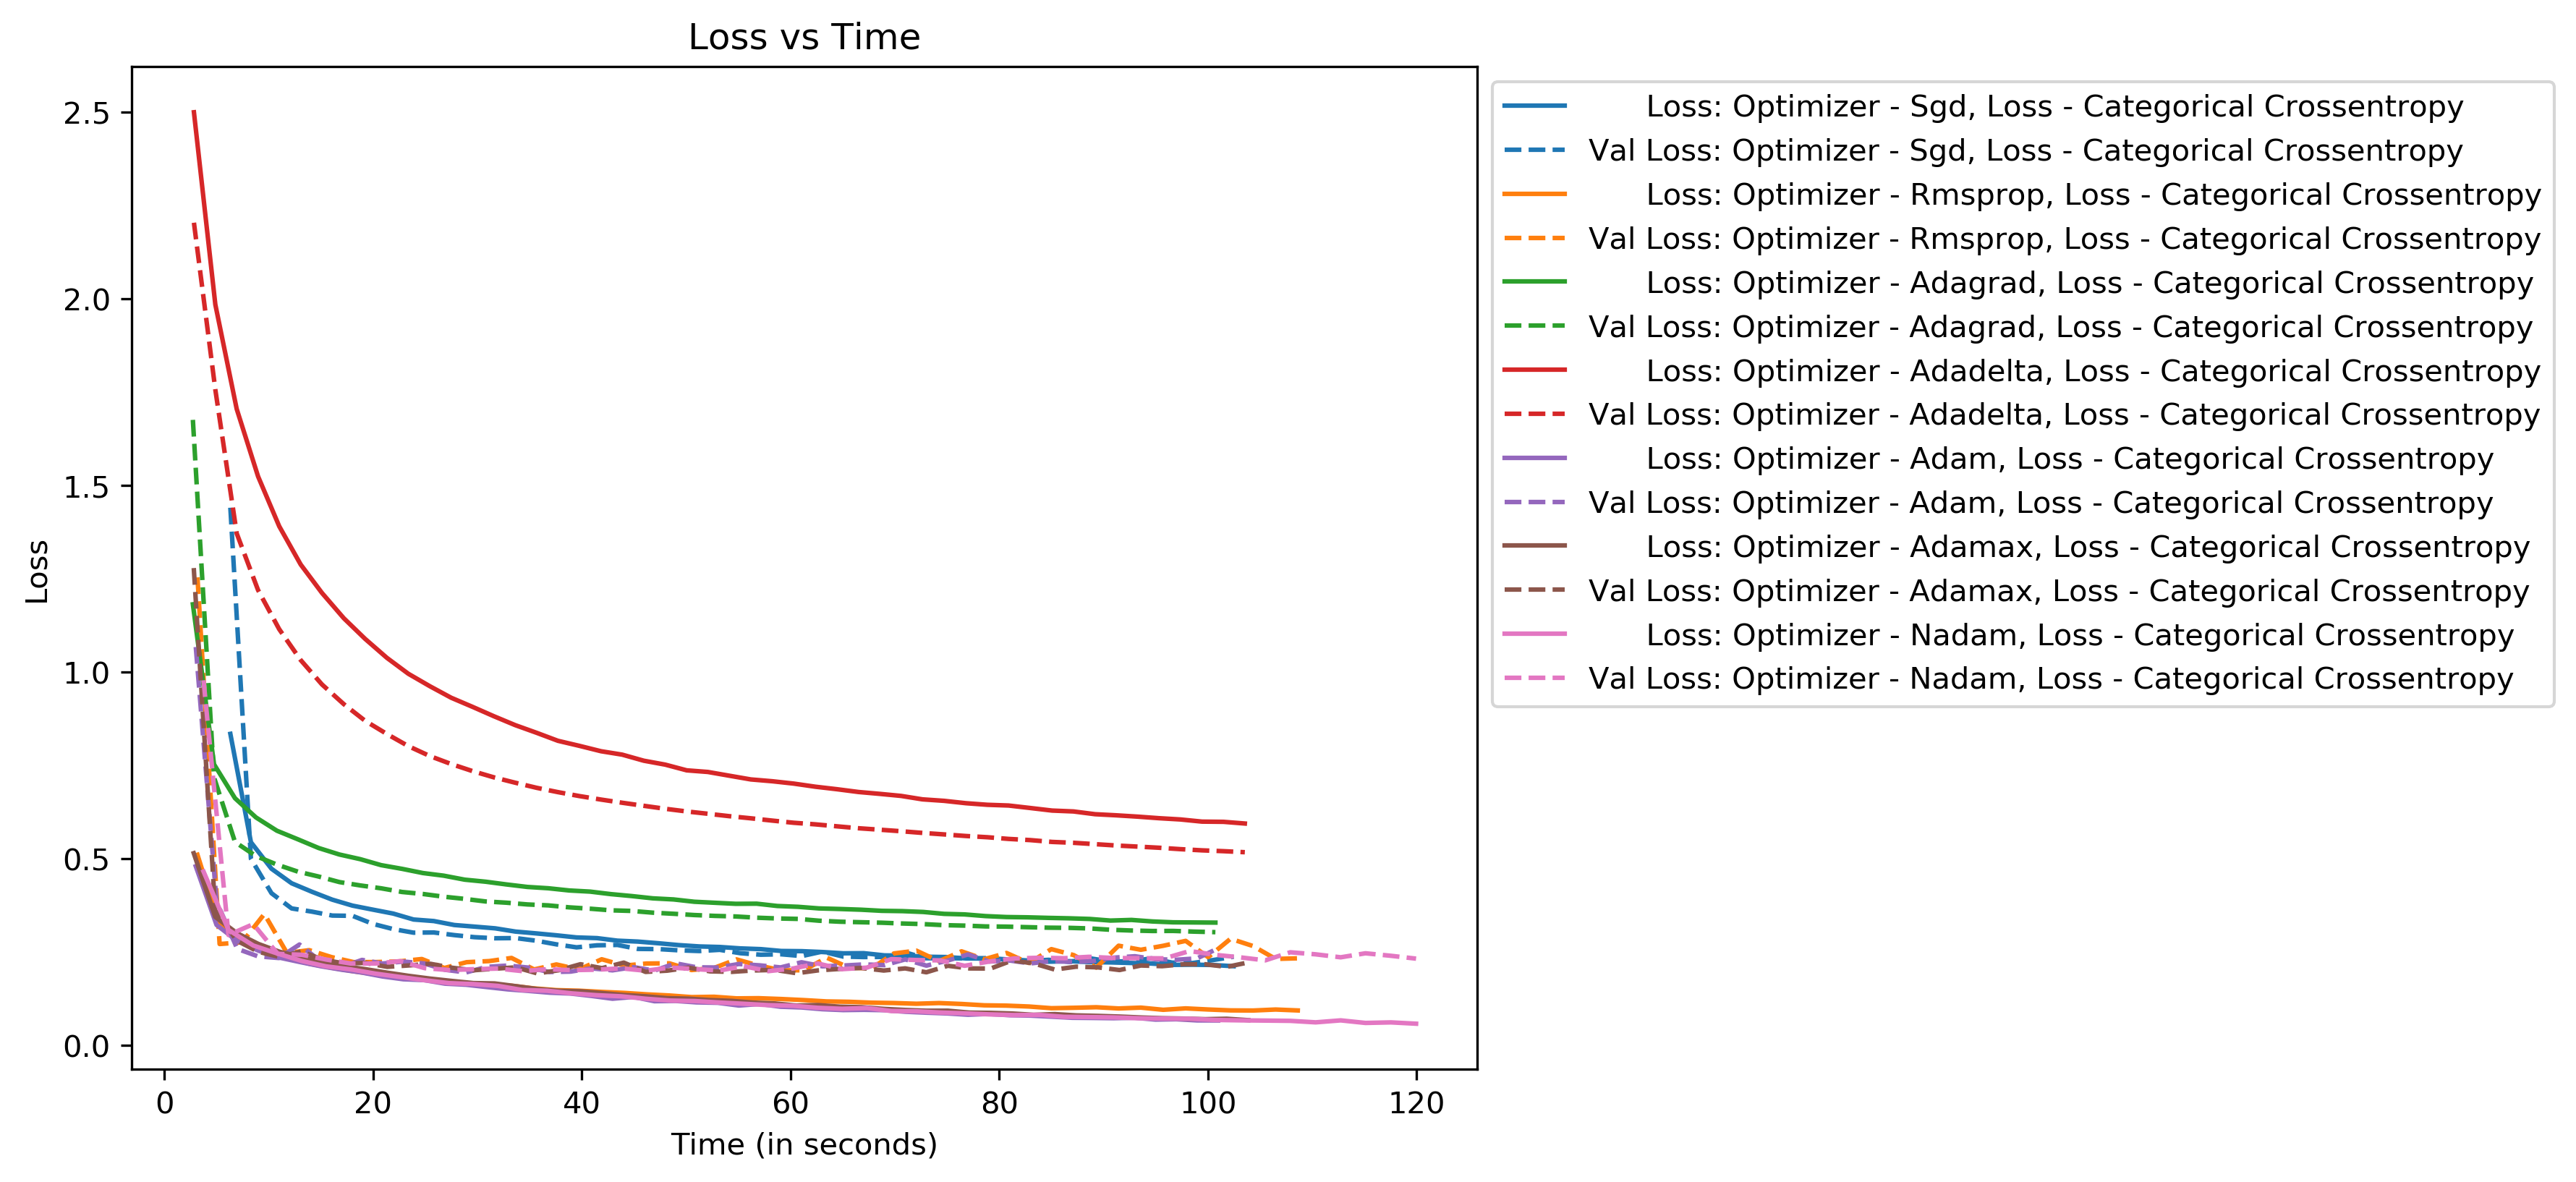
\includegraphics[width=\linewidth]{task_4_loss_time.png}
  \caption{Loss of MCNN using different optimizers over time.}
  \label{fig:task_4_loss_time}
\end{figure}

\begin{figure}
  \centering
  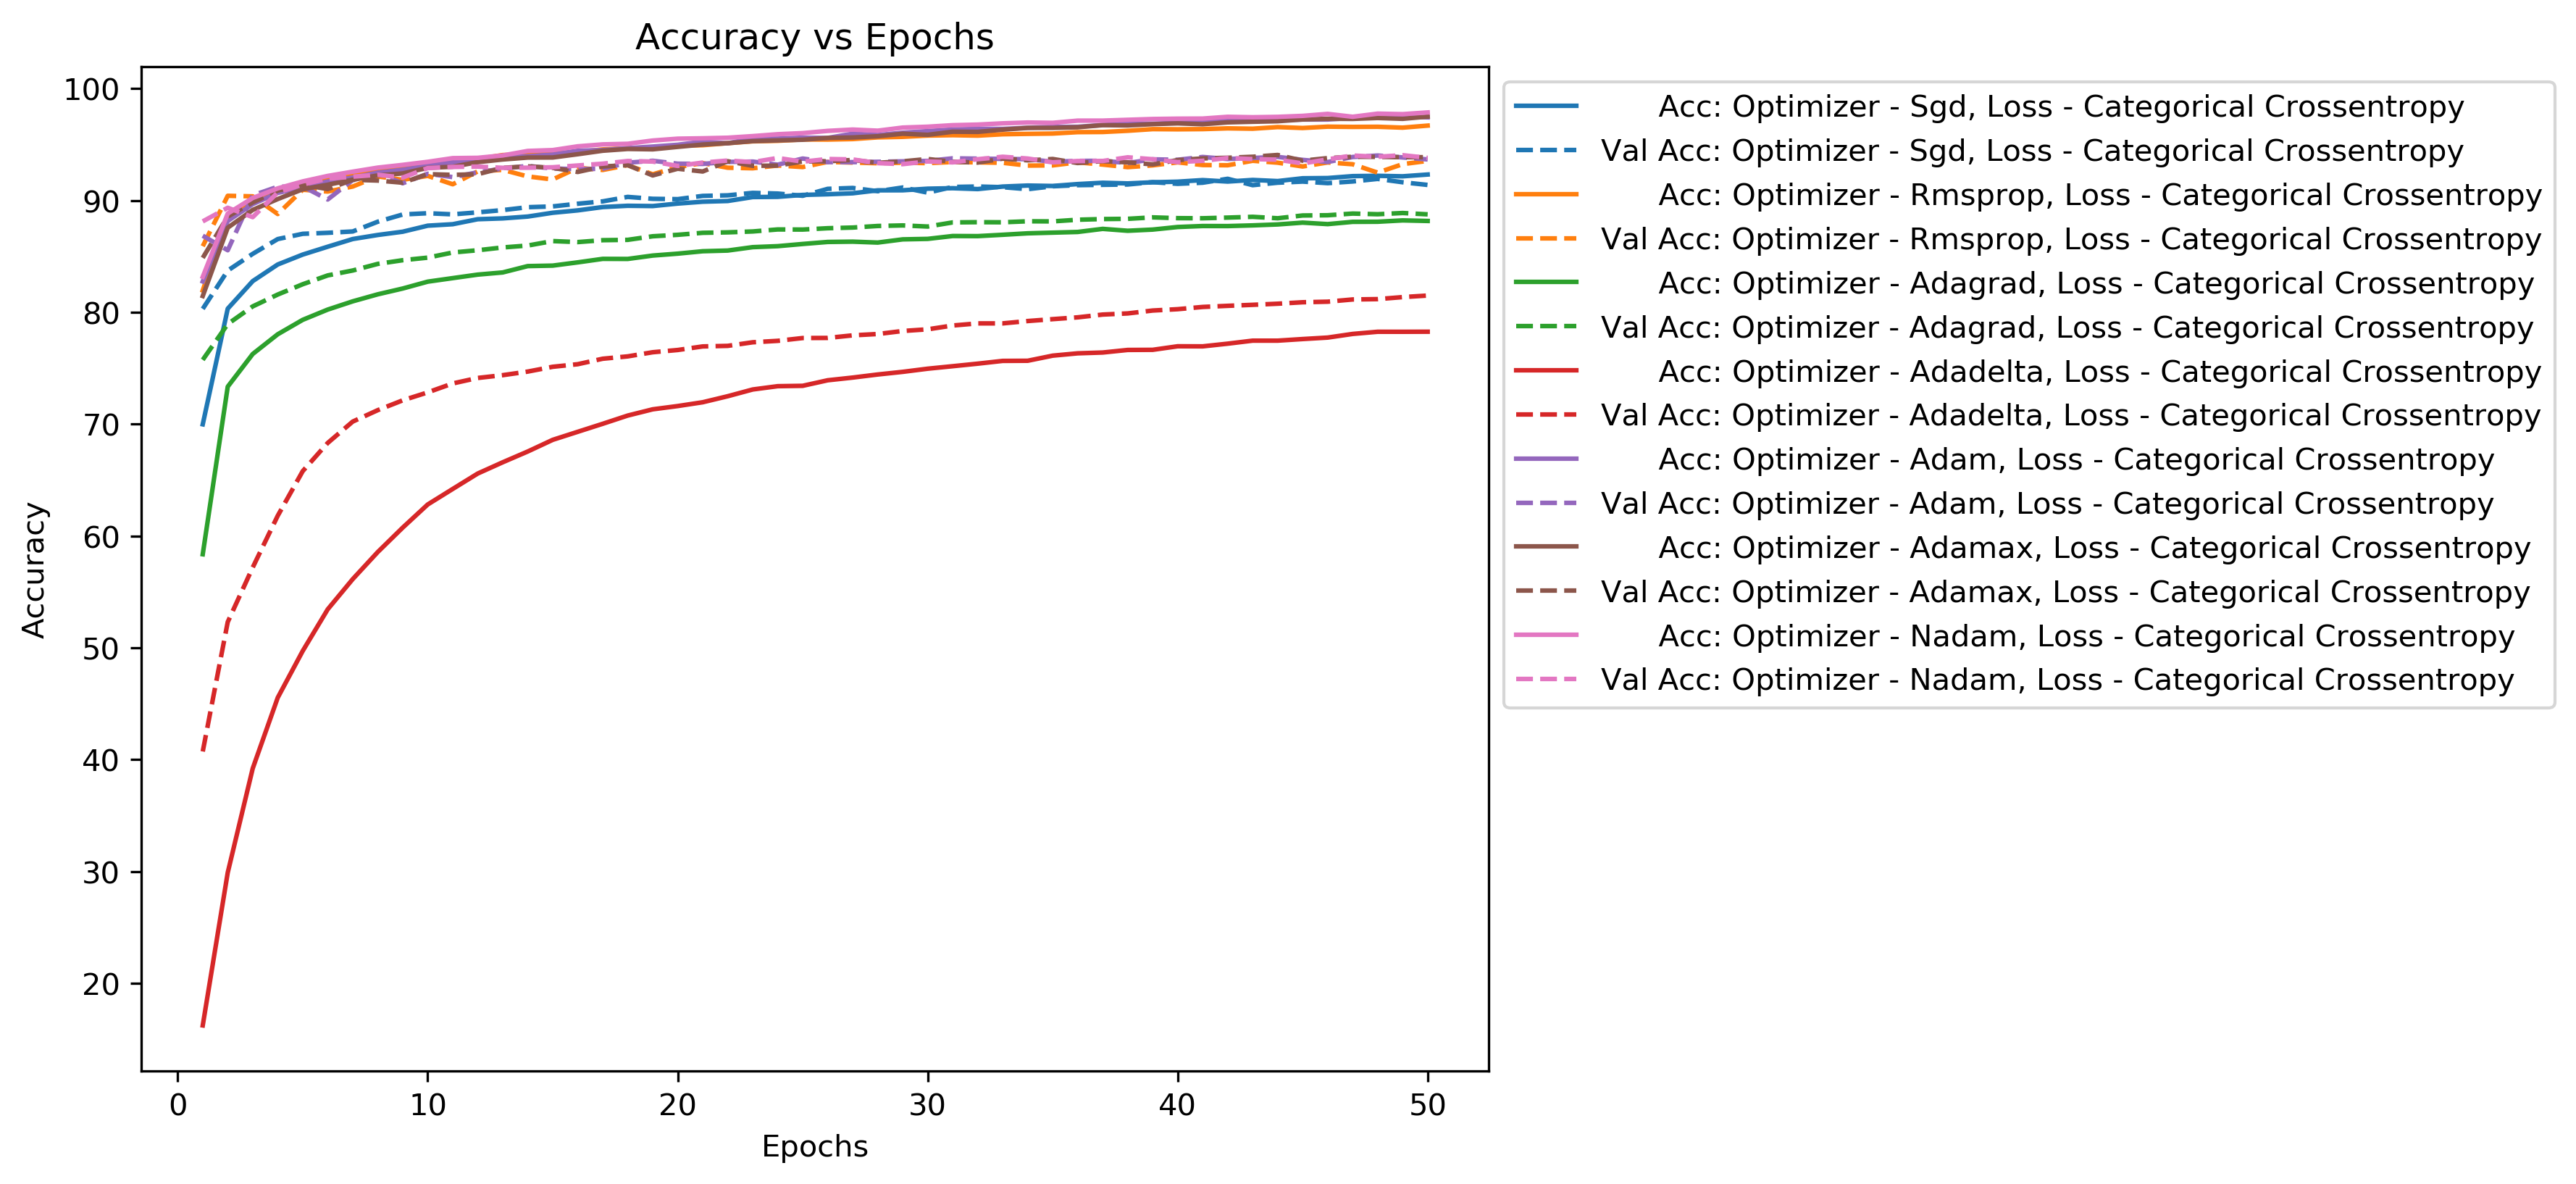
\includegraphics[width=\linewidth]{task_4_acc_epochs.png}
  \caption{Accuracy of MCNN using different optimizers over time.}
  \label{fig:task_4_acc_epochs}
\end{figure}

\begin{figure}
  \centering
  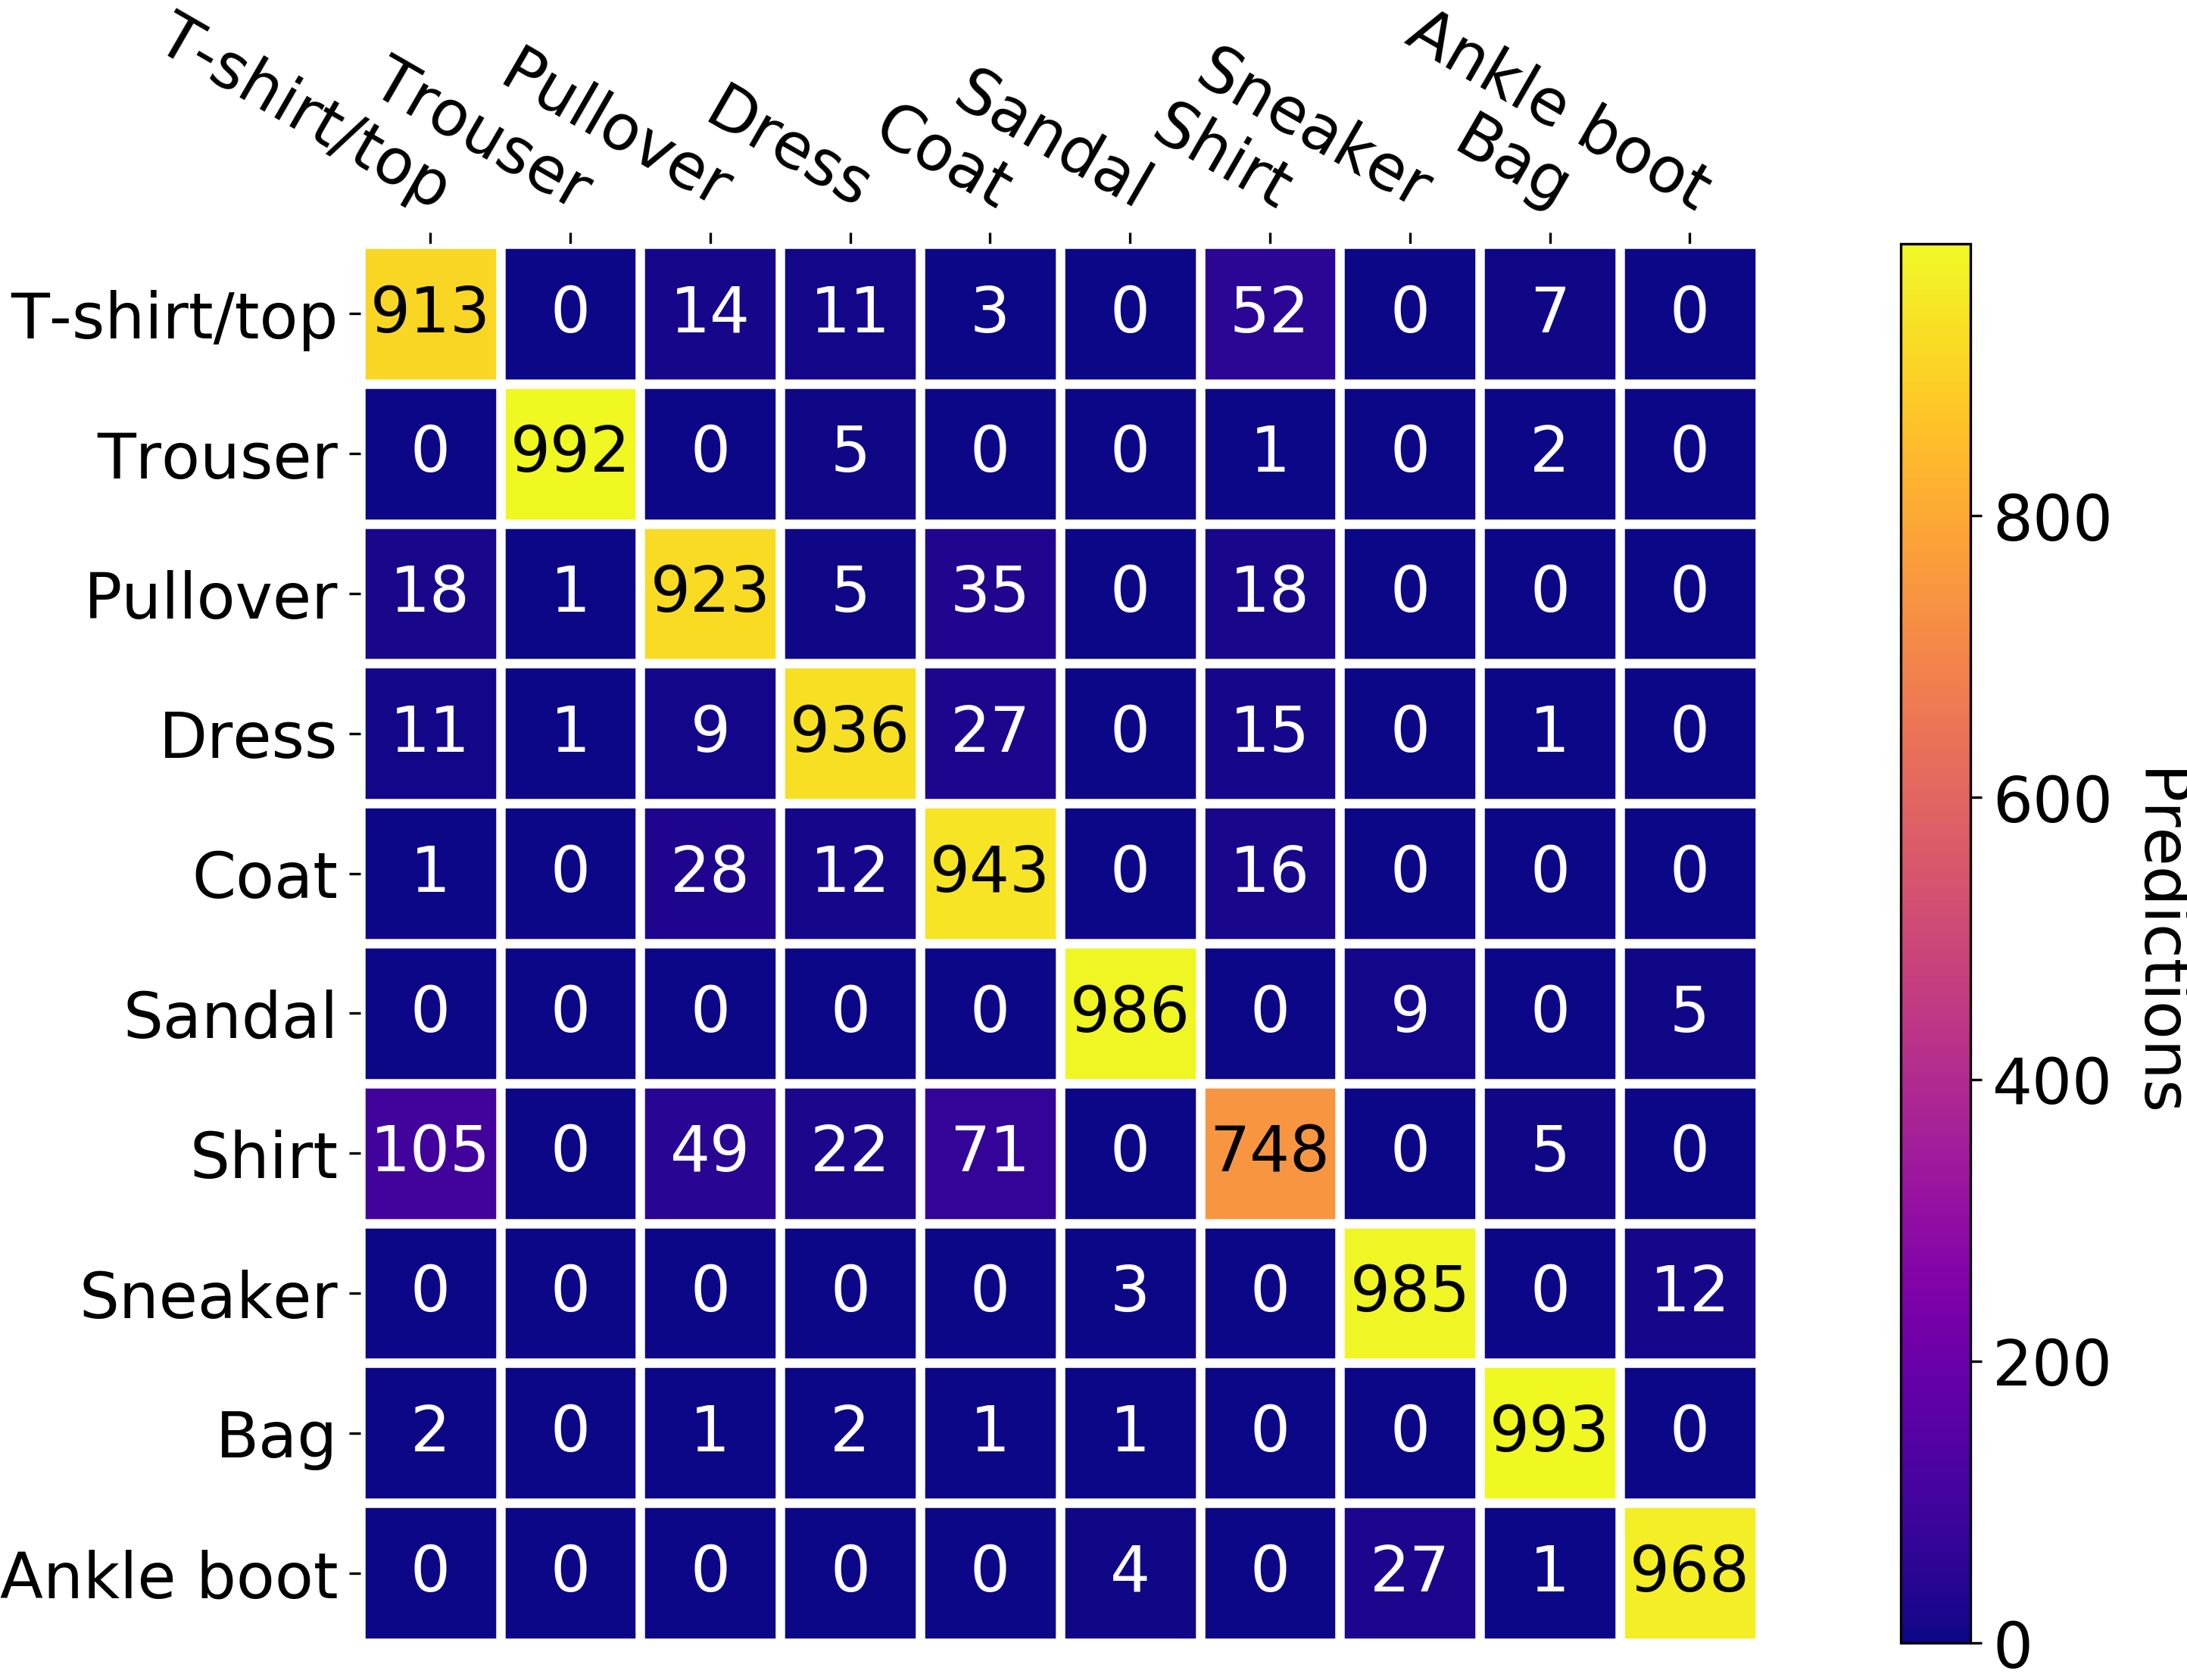
\includegraphics[width=\linewidth]{task_4_cm.png}
  \caption{MCNN Confusion Matrix as a heatmap. Brighter diagonal means the NN did better. Any cell off
   the diagonal that is bright represents severe misclassification. Rows are predictions, columns are ground truth.}
  \label{fig:task_4_cm}
\end{figure}

\begin{table}[]
  \centering
  \caption{Accuracy across optimizers on MCNN.}
  \label{tab:MCNN}
  \begin{tabular}{|c|c|c|c|c|c|c|c|}
  \hline
   & SGD & RMSprop & Adagrad & Adadelta & Adam & Adamax & Nadam \\ \hline
   Categorical C.E. & 91.39\% & 93.55\% & 88.76\% & 81.50\% & 93.67\% & \textbf{93.87\%} & 93.81\% \\ \hline
  \end{tabular}
  \end{table}


\subsection{Variational Auto Encoder}

Because the VAE doesn't perform classification, we can't really compare it to the any of the previous models.
The best we can do is compare the clothes is produces to the quality of the original ones, both visually and relative to another VAE.
Because we're testing optimizers and their performance on reducing loss, we can look at
 Figure \ref{fig:task_5_loss_epochs_1} and \ref{fig:task_5_loss_time_1} to see how they stack up.
Unlike the classification networks, only one optimizer, Adadelta, got a slow start and never managed to catch up.
All of the other six performed comparably.

In Table \ref{tab:VAE_1}, we can see that the final loss for all of them was in the mid to low 20s.
Nadam barely beat the rest at 23.45, while Adadelta performed poorly at 37.61.

In Figure \ref{fig:task_5_clothes_kernel_3_kernels_16_latent_5}, we iterate over each column of the latent vector to
 look at two things: a) do all of the columns matter, and b) what does each contribute?
For VAE$_1$, it seems that all of the columns contribute something different and we can visually see that each one targets a different class
 from the training data.
In Figure \ref{fig:task_5_clothes_kernel_3_kernels_16_latent_5_examples}, we can see some clothes that were
 generated using random latent vectors and all of them look real and as if they could have come from our training set.


Now we can look at the performance of our second VAE and compare the two.
First, let's look at the optimizers and their performance on reducing loss in
 Figure \ref{fig:task_5_loss_epochs_2} and \ref{fig:task_5_loss_time_2}.
Adadelta and Adagrad get off to a slow start and never manage to catch back up.
But something especially weird happened.
Nadam and SGD never converge to a low loss.
They seem to get stuck in a local minimum early on and never manage to get out.
In order to verify this is true, we reran this network 5 times and each time, the exact same thing happened.
They both got stuck and never converged any further.
The last three all perform comparably.

In Table \ref{tab:VAE_2}, we can see that the final loss for the best four was all in the mid to low 20s.
SGD got stuck at a very high 97.39 and Nadam got stuck at a still very high 67.98.
This time, Adamax took home the trophy at a low 22.83.

In Figure \ref{fig:task_5_clothes_kernel_5_kernels_32_latent_10}, we iterate over each column of the latent vector.
For VAE$_2$, it seems that not all of the columns contribute something different and we can visually see that some target the
 same classes from the training data.
This might mean that a latent vector of 10 is unnecessary and too large for this problem.
In Figure \ref{fig:task_5_clothes_kernel_5_kernels_32_latent_10_examples}, we can see some clothes that were
 generated using random latent vectors and like VAE$_1$, all of them look real and as if they could have come from our training set.

\begin{figure}
  \centering
  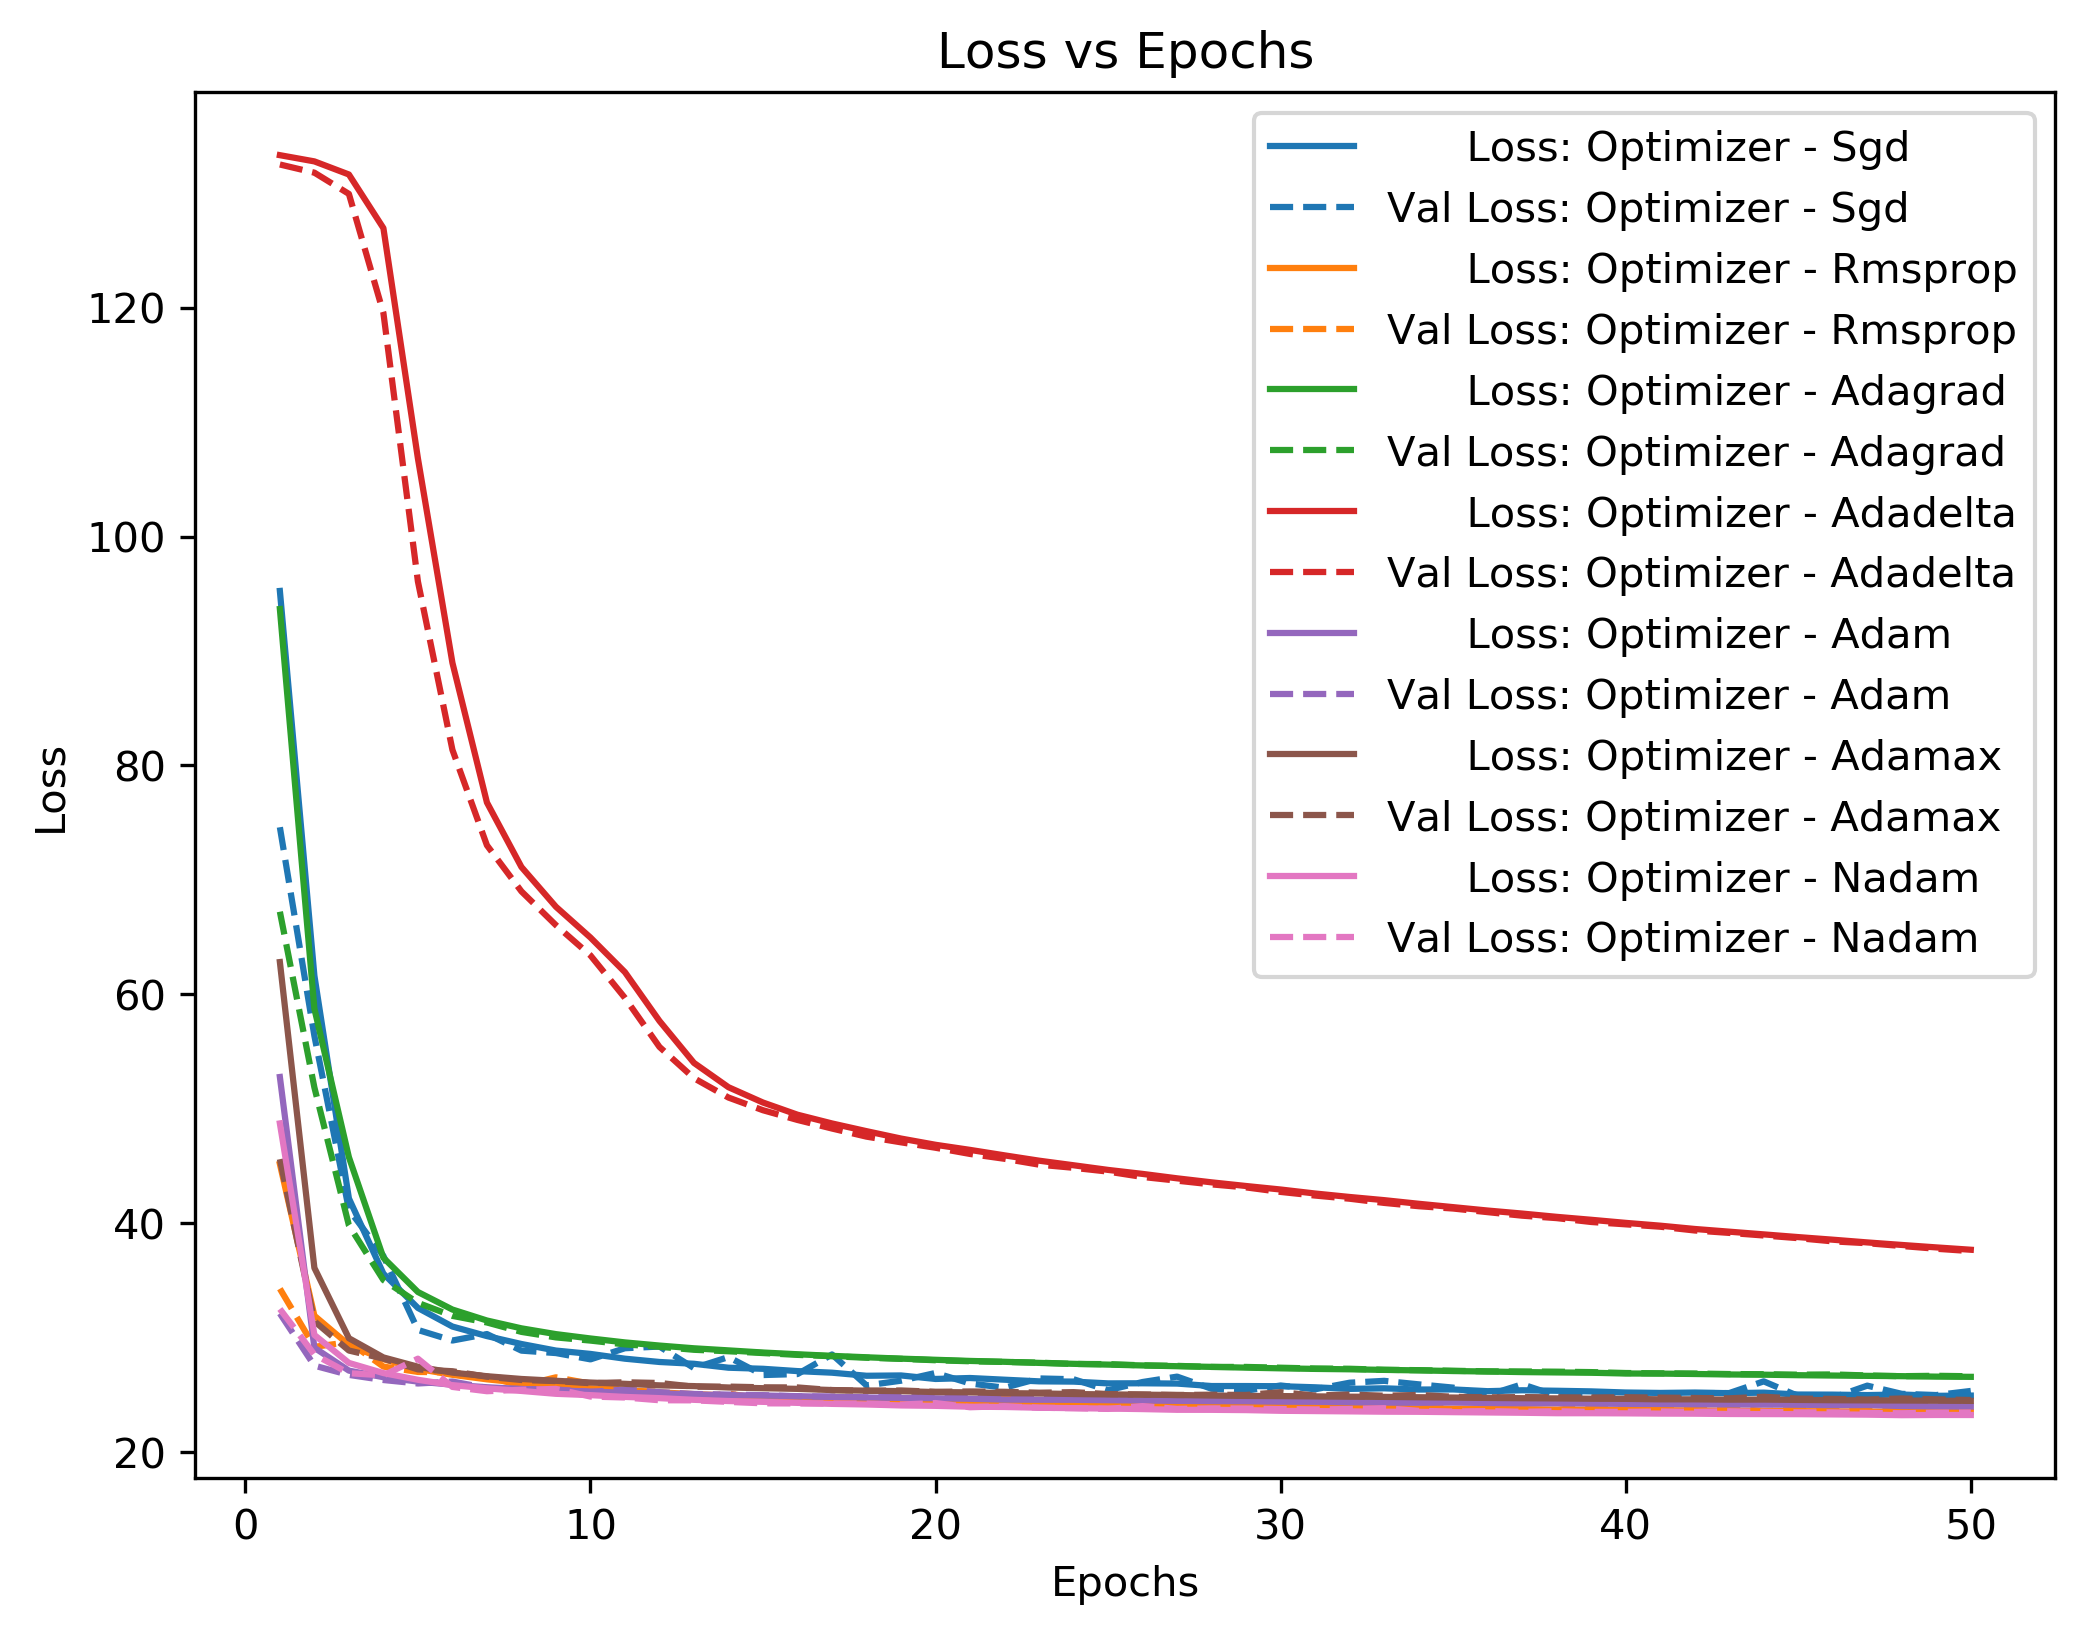
\includegraphics[width=\linewidth]{task_5_loss_epochs.png}
  \caption{Loss of VAE$_1$ using different optimizers over epochs.}
  \label{fig:task_5_loss_epochs_1}
\end{figure}

\begin{figure}
  \centering
  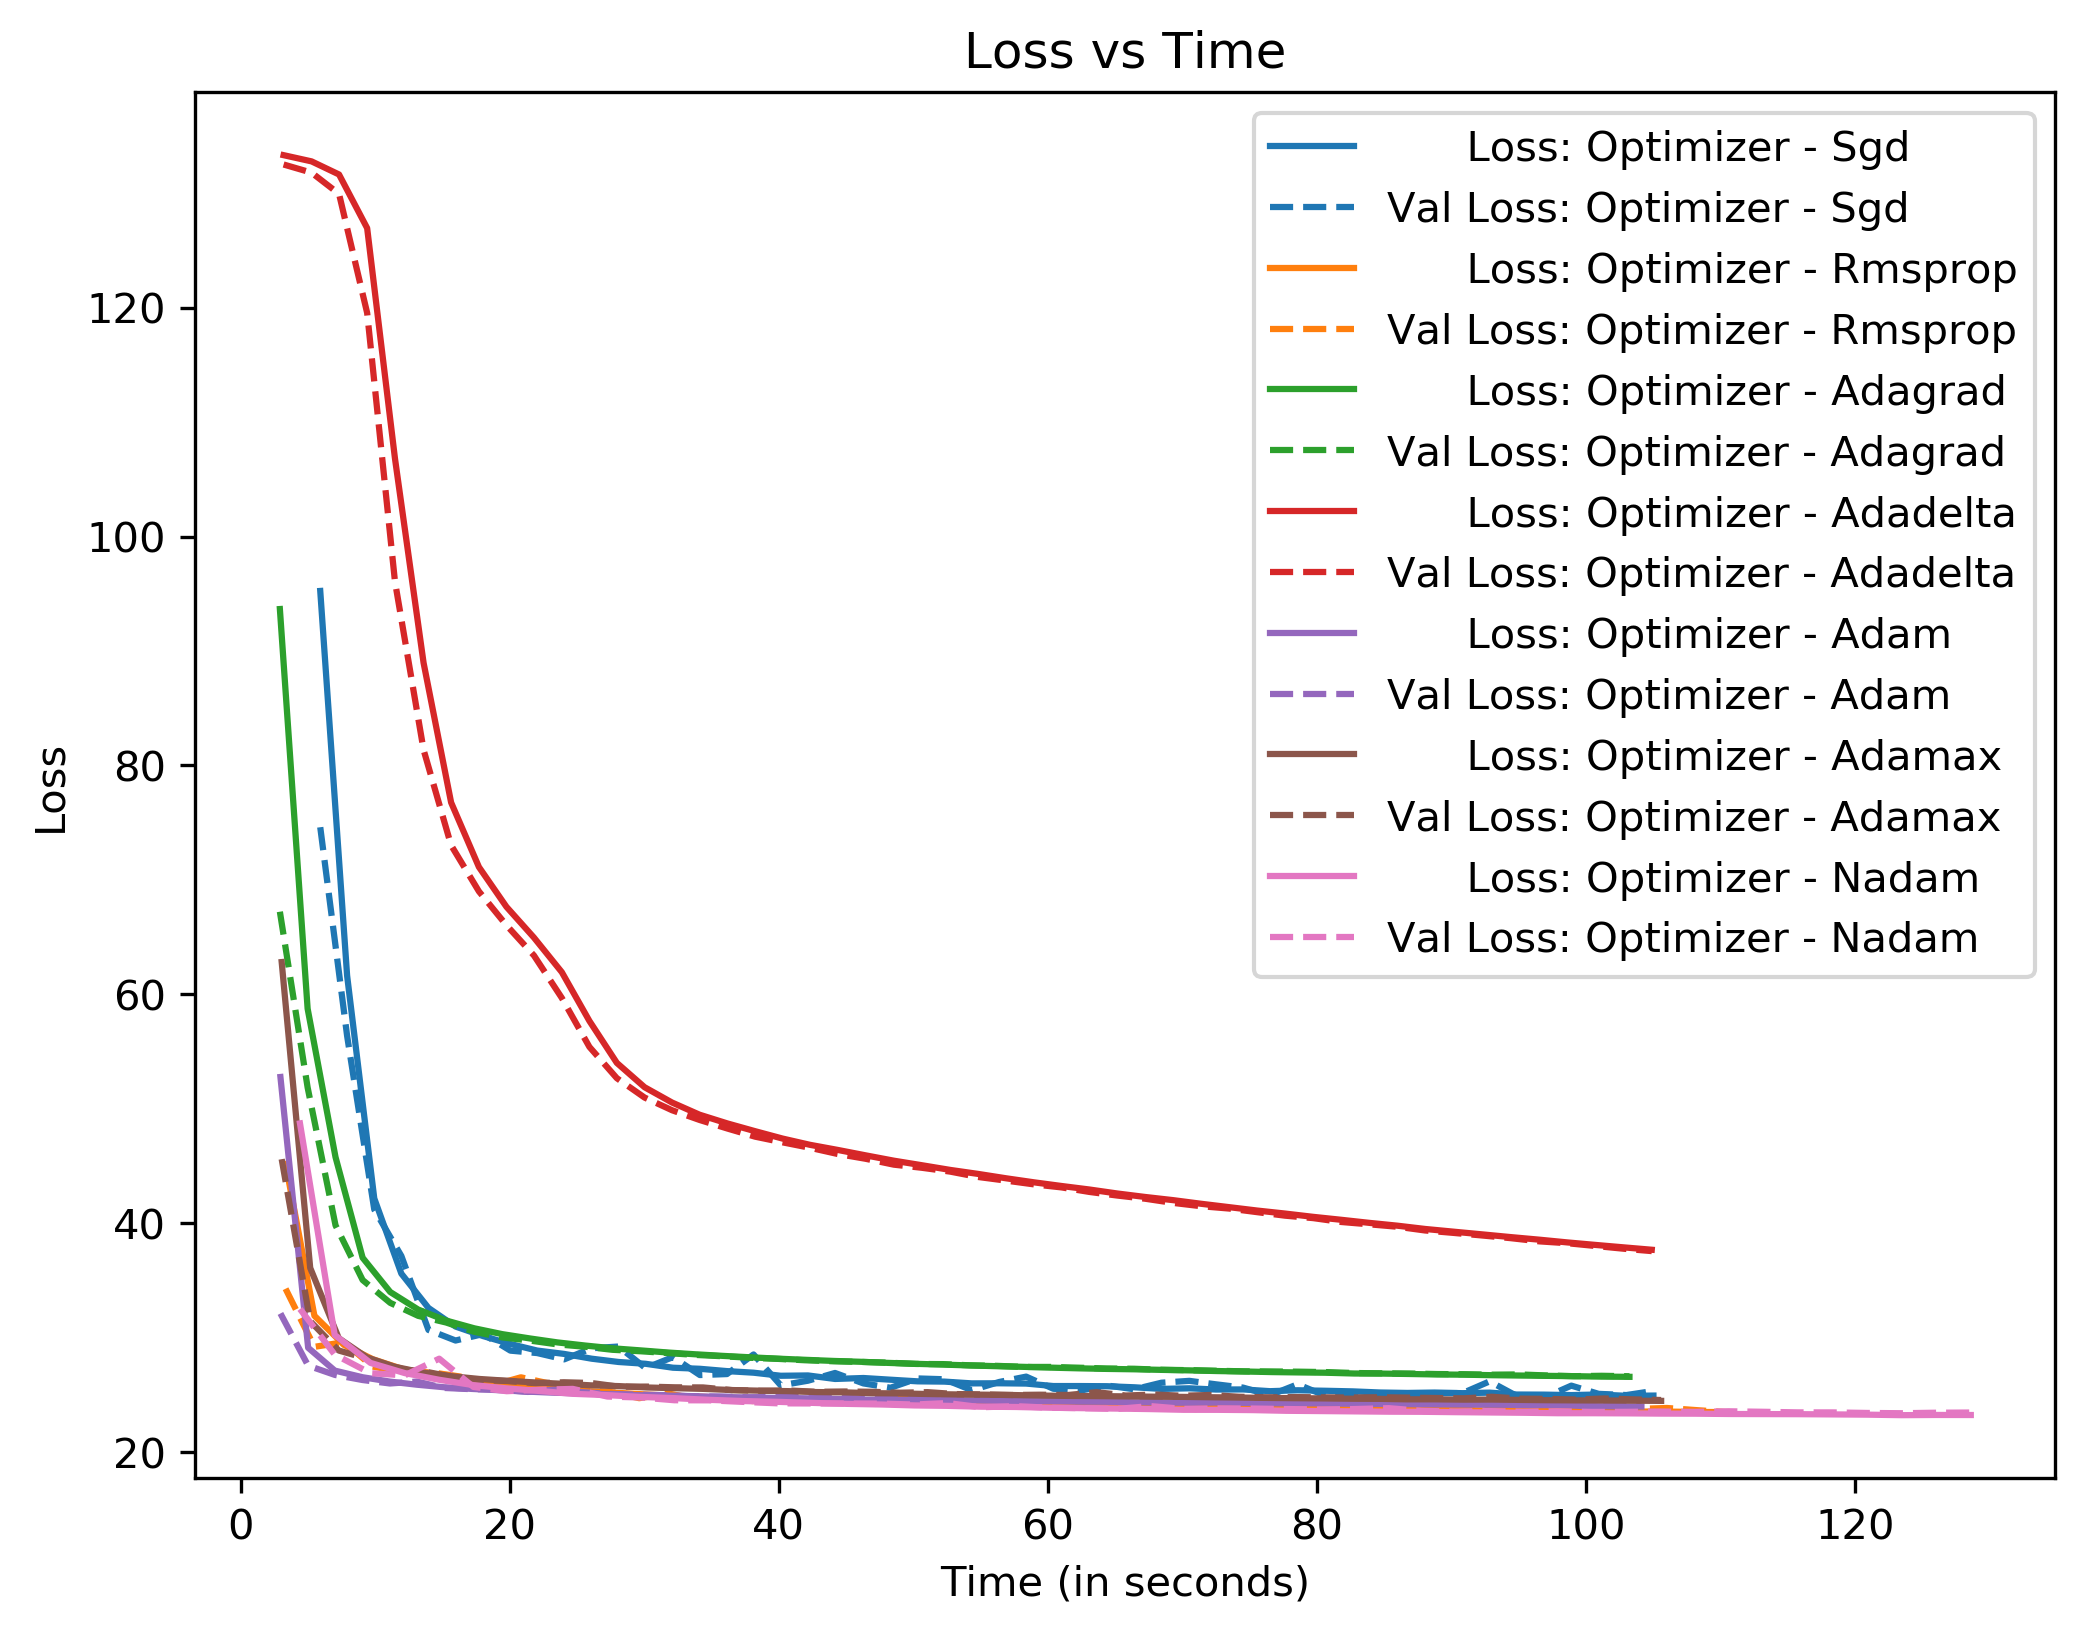
\includegraphics[width=\linewidth]{task_5_loss_time.png}
  \caption{Loss of VAE$_1$ using different optimizers over time.}
  \label{fig:task_5_loss_time_1}
\end{figure}

\begin{figure}
  \centering
  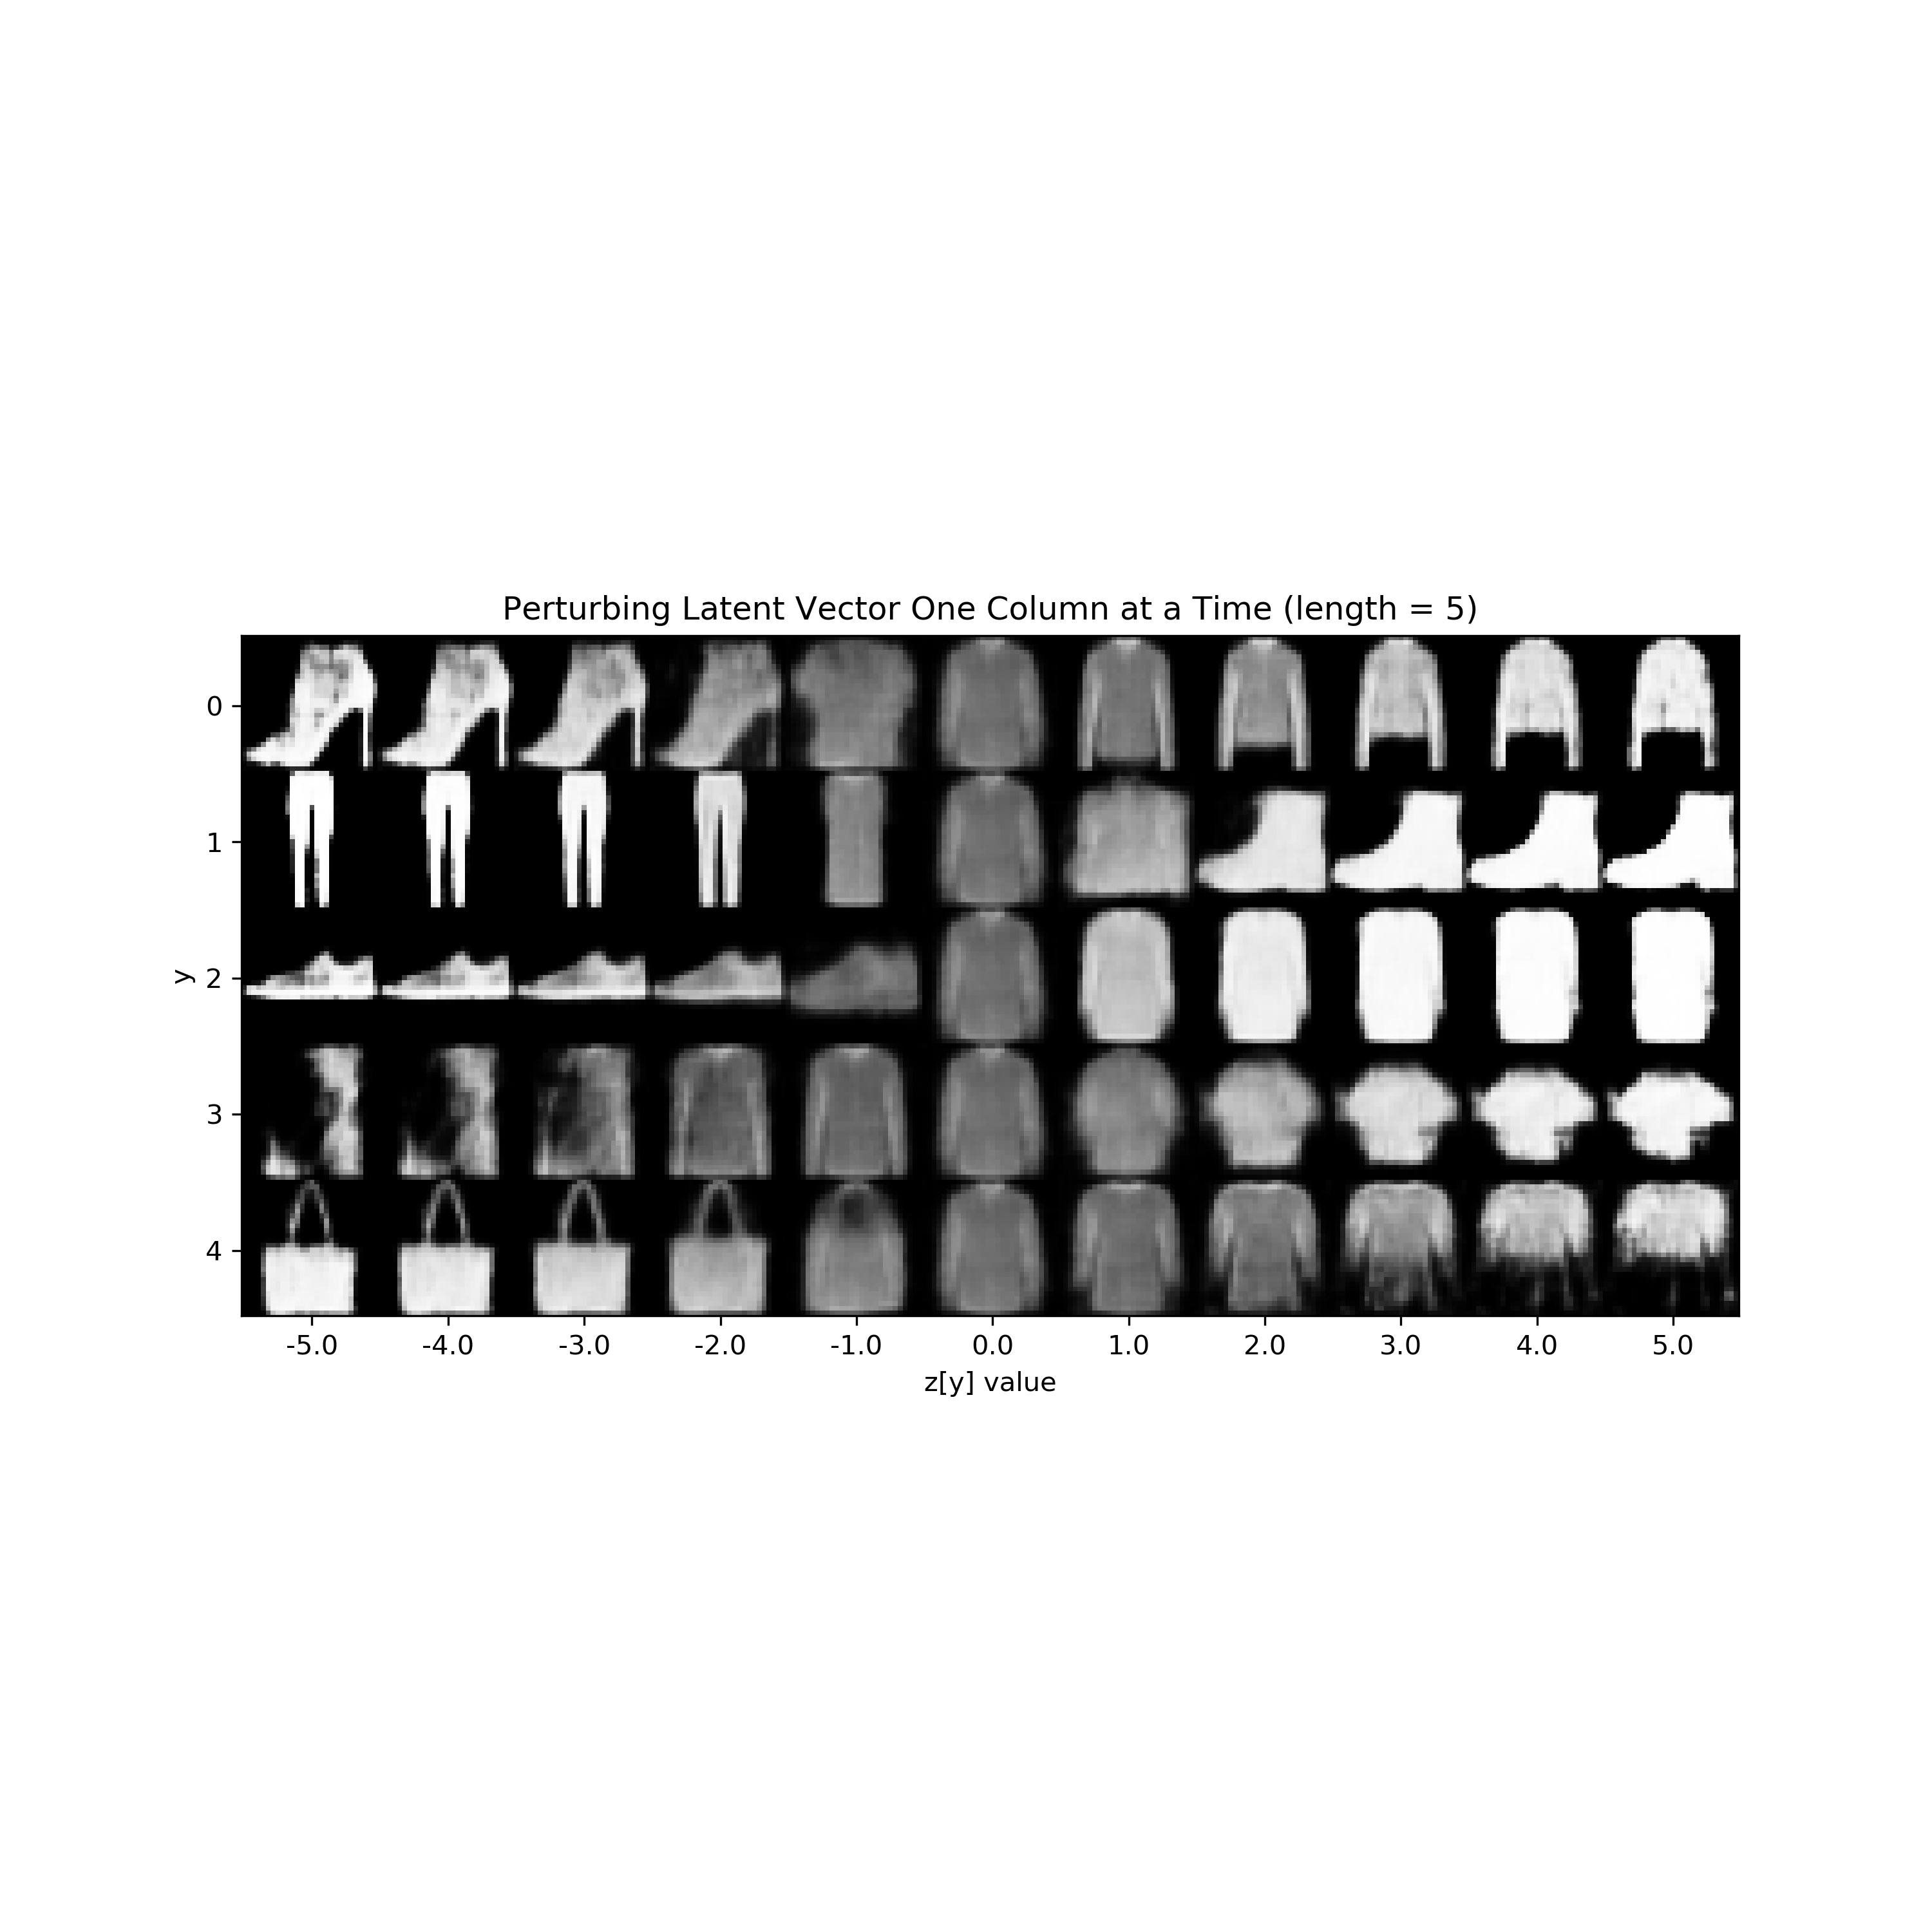
\includegraphics[width=\linewidth]{task_5_clothes_kernel_3_kernels_16_latent_5.png}
  \caption{Clothes generated using VAE$_1$'s decoder after walking over each latent dimension iteratively.}
  \label{fig:task_5_clothes_kernel_3_kernels_16_latent_5}
\end{figure}

\begin{figure}
  \centering
  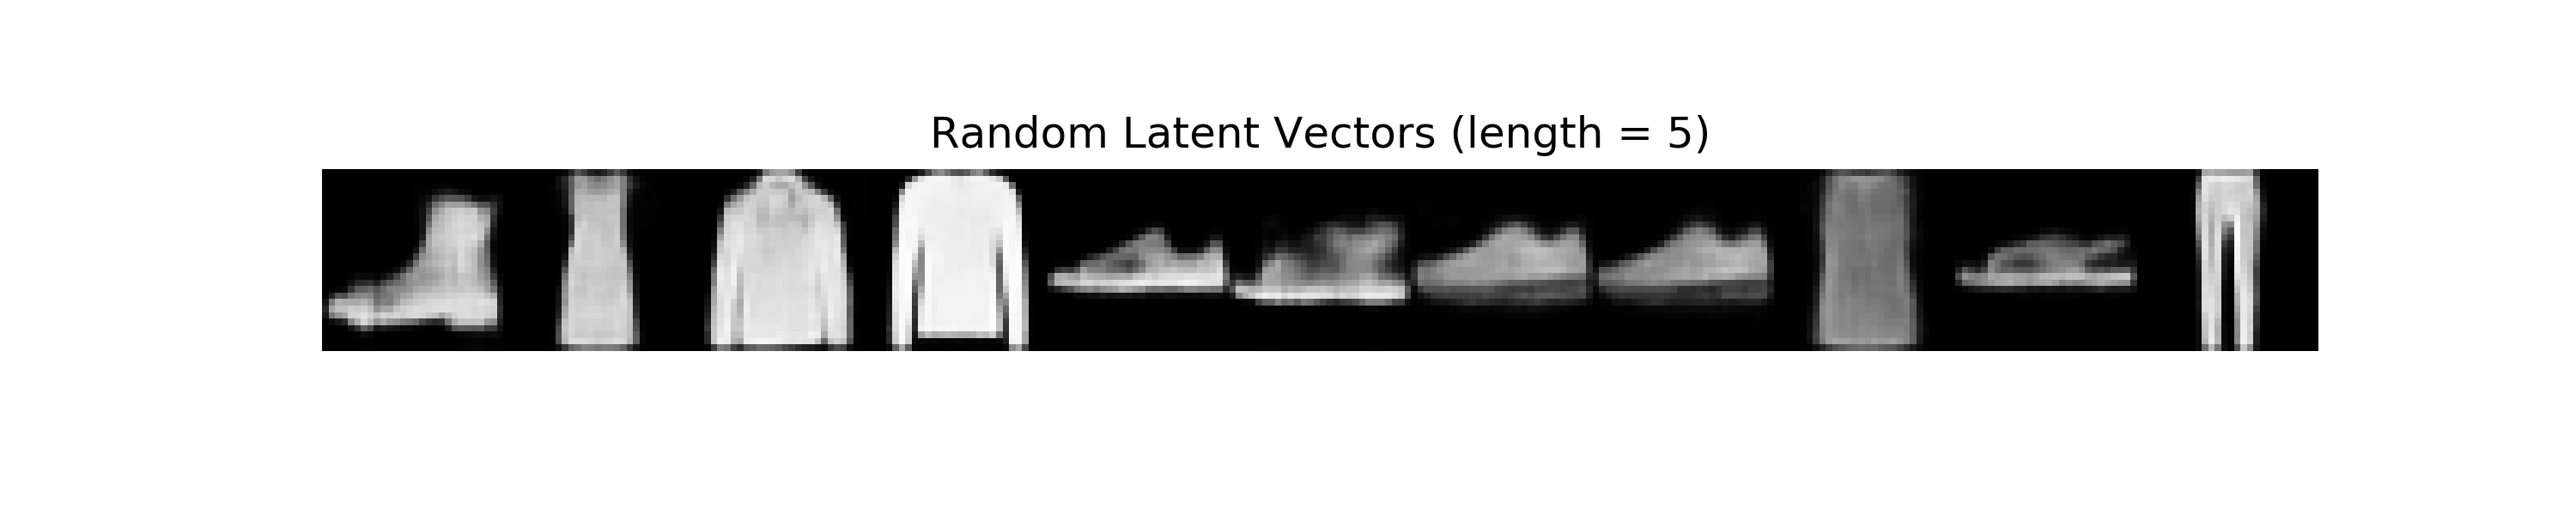
\includegraphics[width=\linewidth]{task_5_clothes_kernel_3_kernels_16_latent_5_examples.png}
  \caption{Clothes generated using VAE$_1$'s decoder using 11 randomly generated latent vectors.}
  \label{fig:task_5_clothes_kernel_3_kernels_16_latent_5_examples}
\end{figure}

\begin{table}[]
  \centering
  \caption{Loss across optimizers on VAE$_1$.}
  \label{tab:VAE_1}
  \begin{tabular}{|c|c|c|c|c|c|c|c|}
  \hline
   & SGD & RMSprop & Adagrad & Adadelta & Adam & Adamax & Nadam \\ \hline
  Mean Squared Error & 25.46 & 23.56 & 26.66 & 37.61 & 24.15 & 24.60 & \textbf{23.45} \\ \hline
  \end{tabular}
  \end{table}

  \begin{figure}
    \centering
    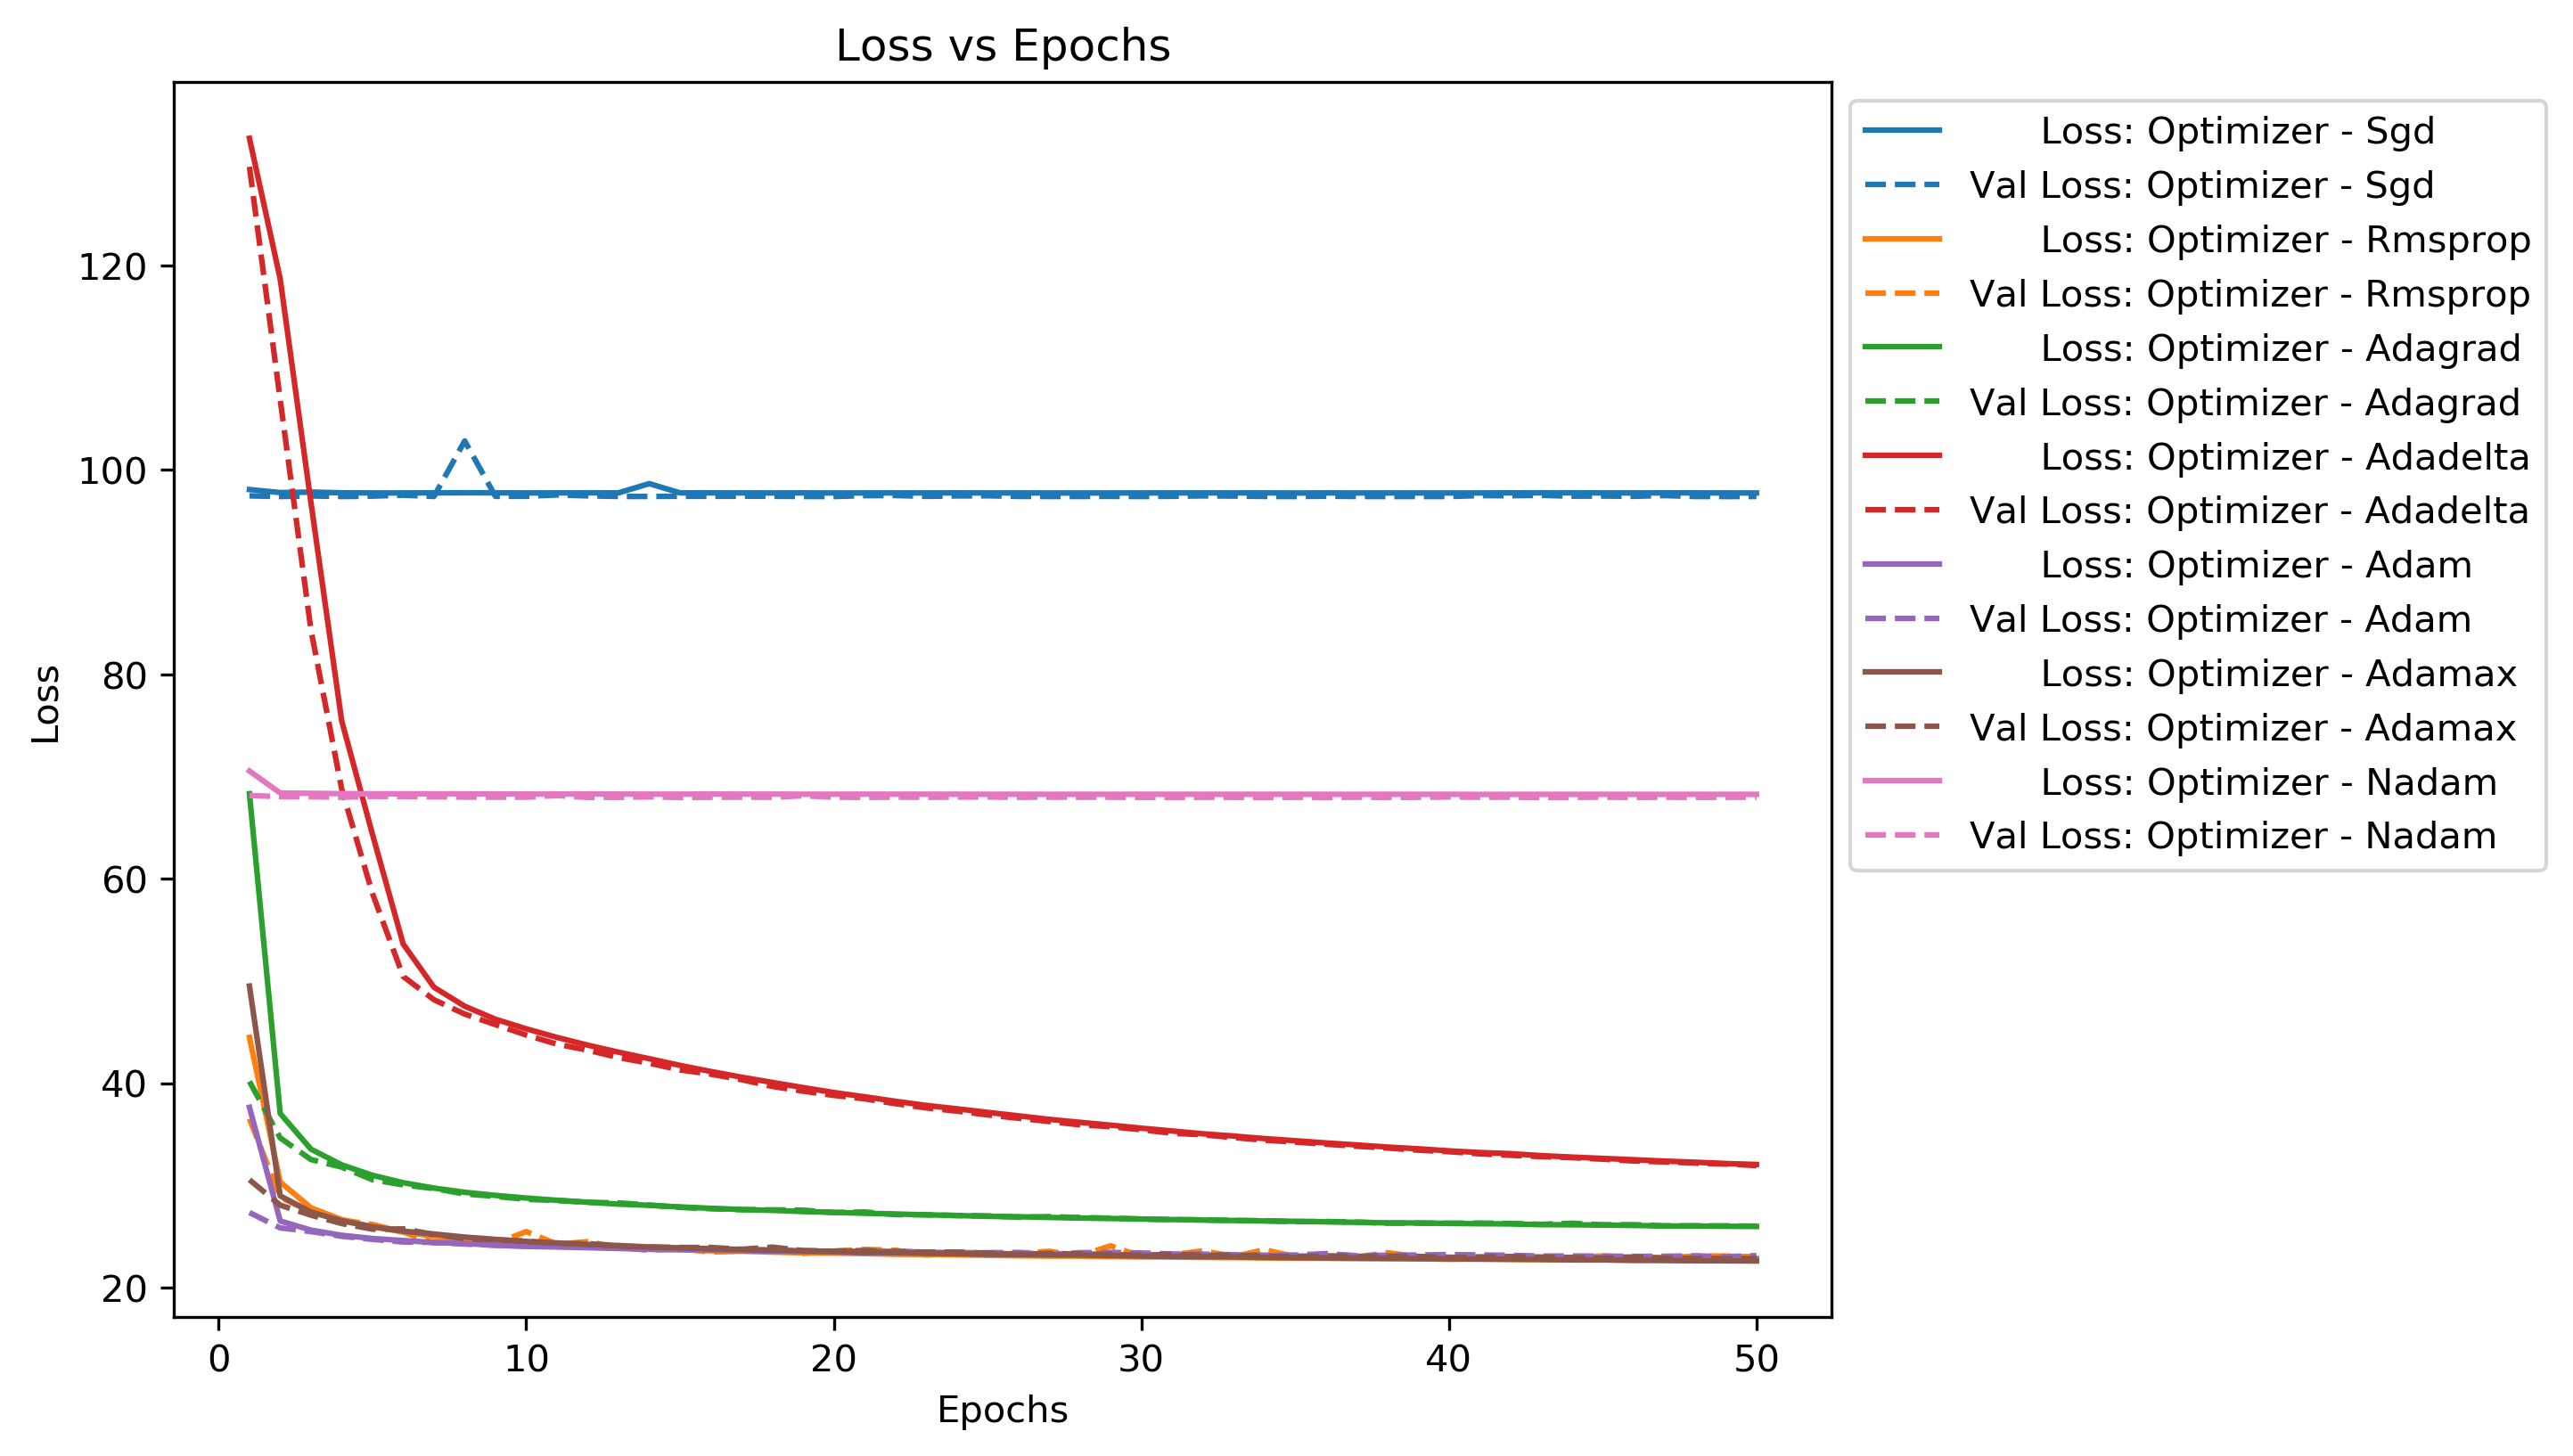
\includegraphics[width=\linewidth]{task_5_loss_epochs_2.png}
    \caption{Loss of VAE$_2$ using different optimizers over epochs.}
    \label{fig:task_5_loss_epochs_2}
  \end{figure}

  \begin{figure}
    \centering
    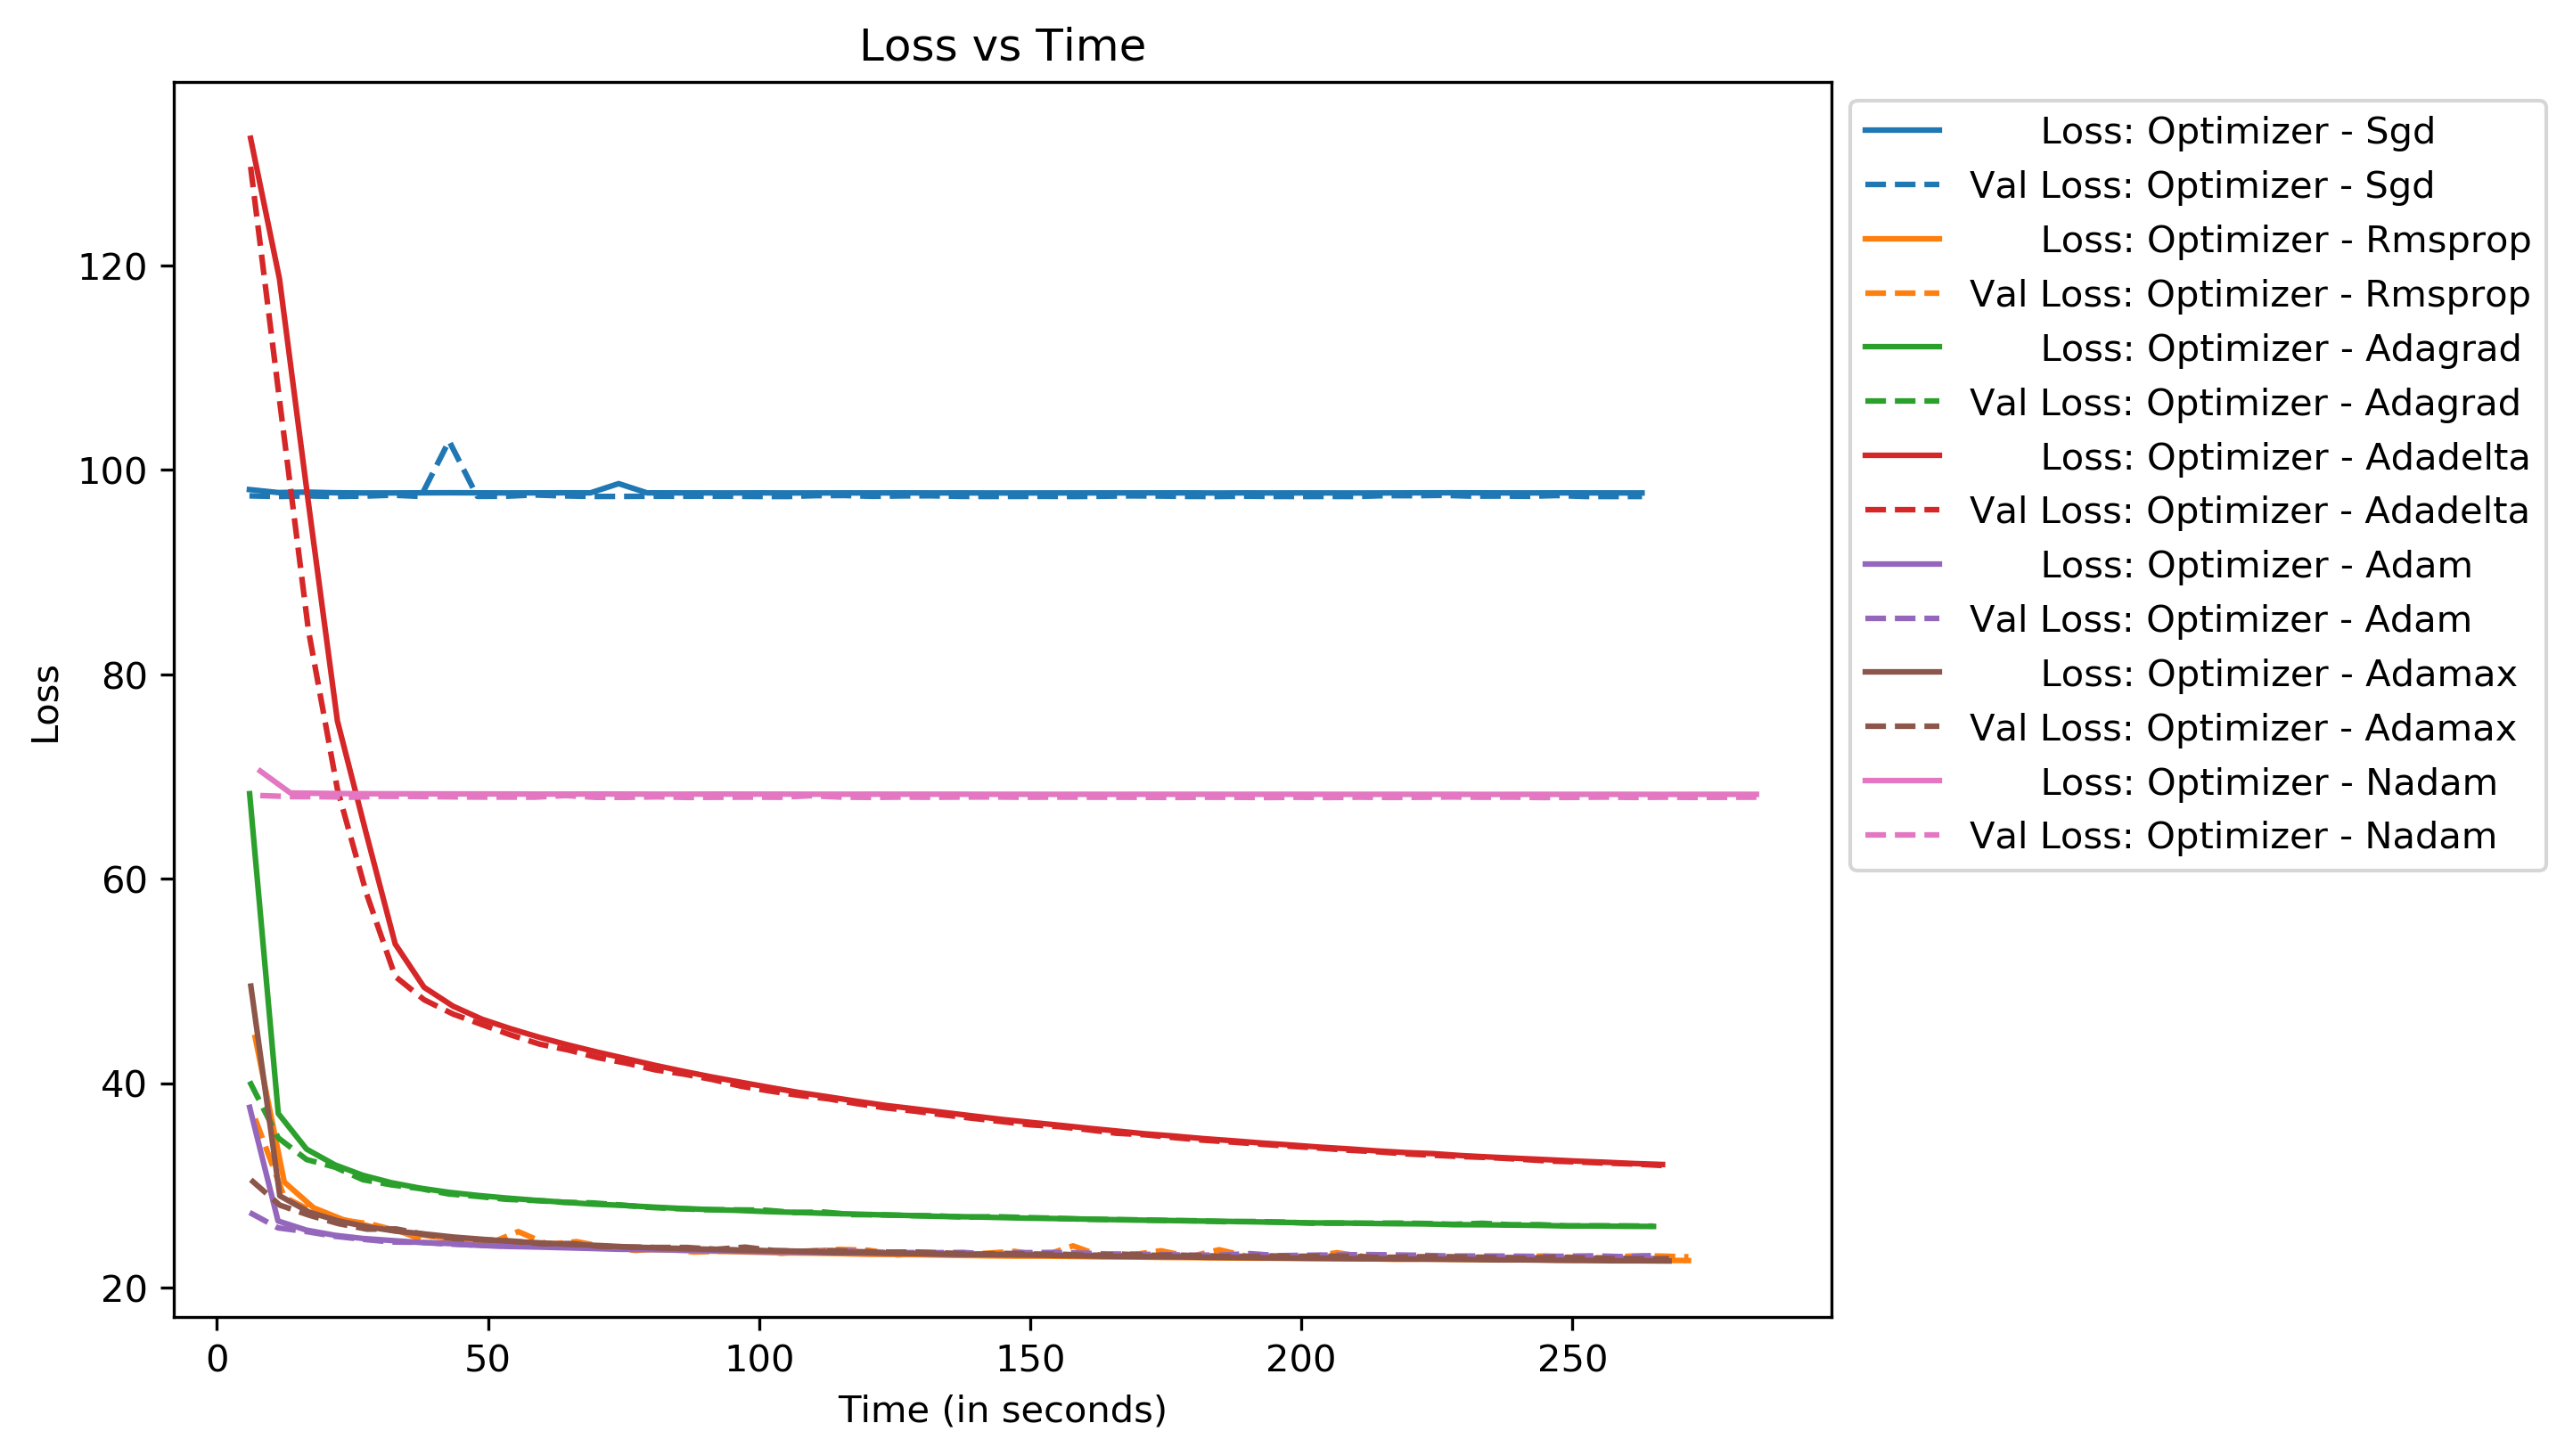
\includegraphics[width=\linewidth]{task_5_loss_time_2.png}
    \caption{Loss of VAE$_2$ using different optimizers over time.}
    \label{fig:task_5_loss_time_2}
  \end{figure}

  \begin{figure}
    \centering
    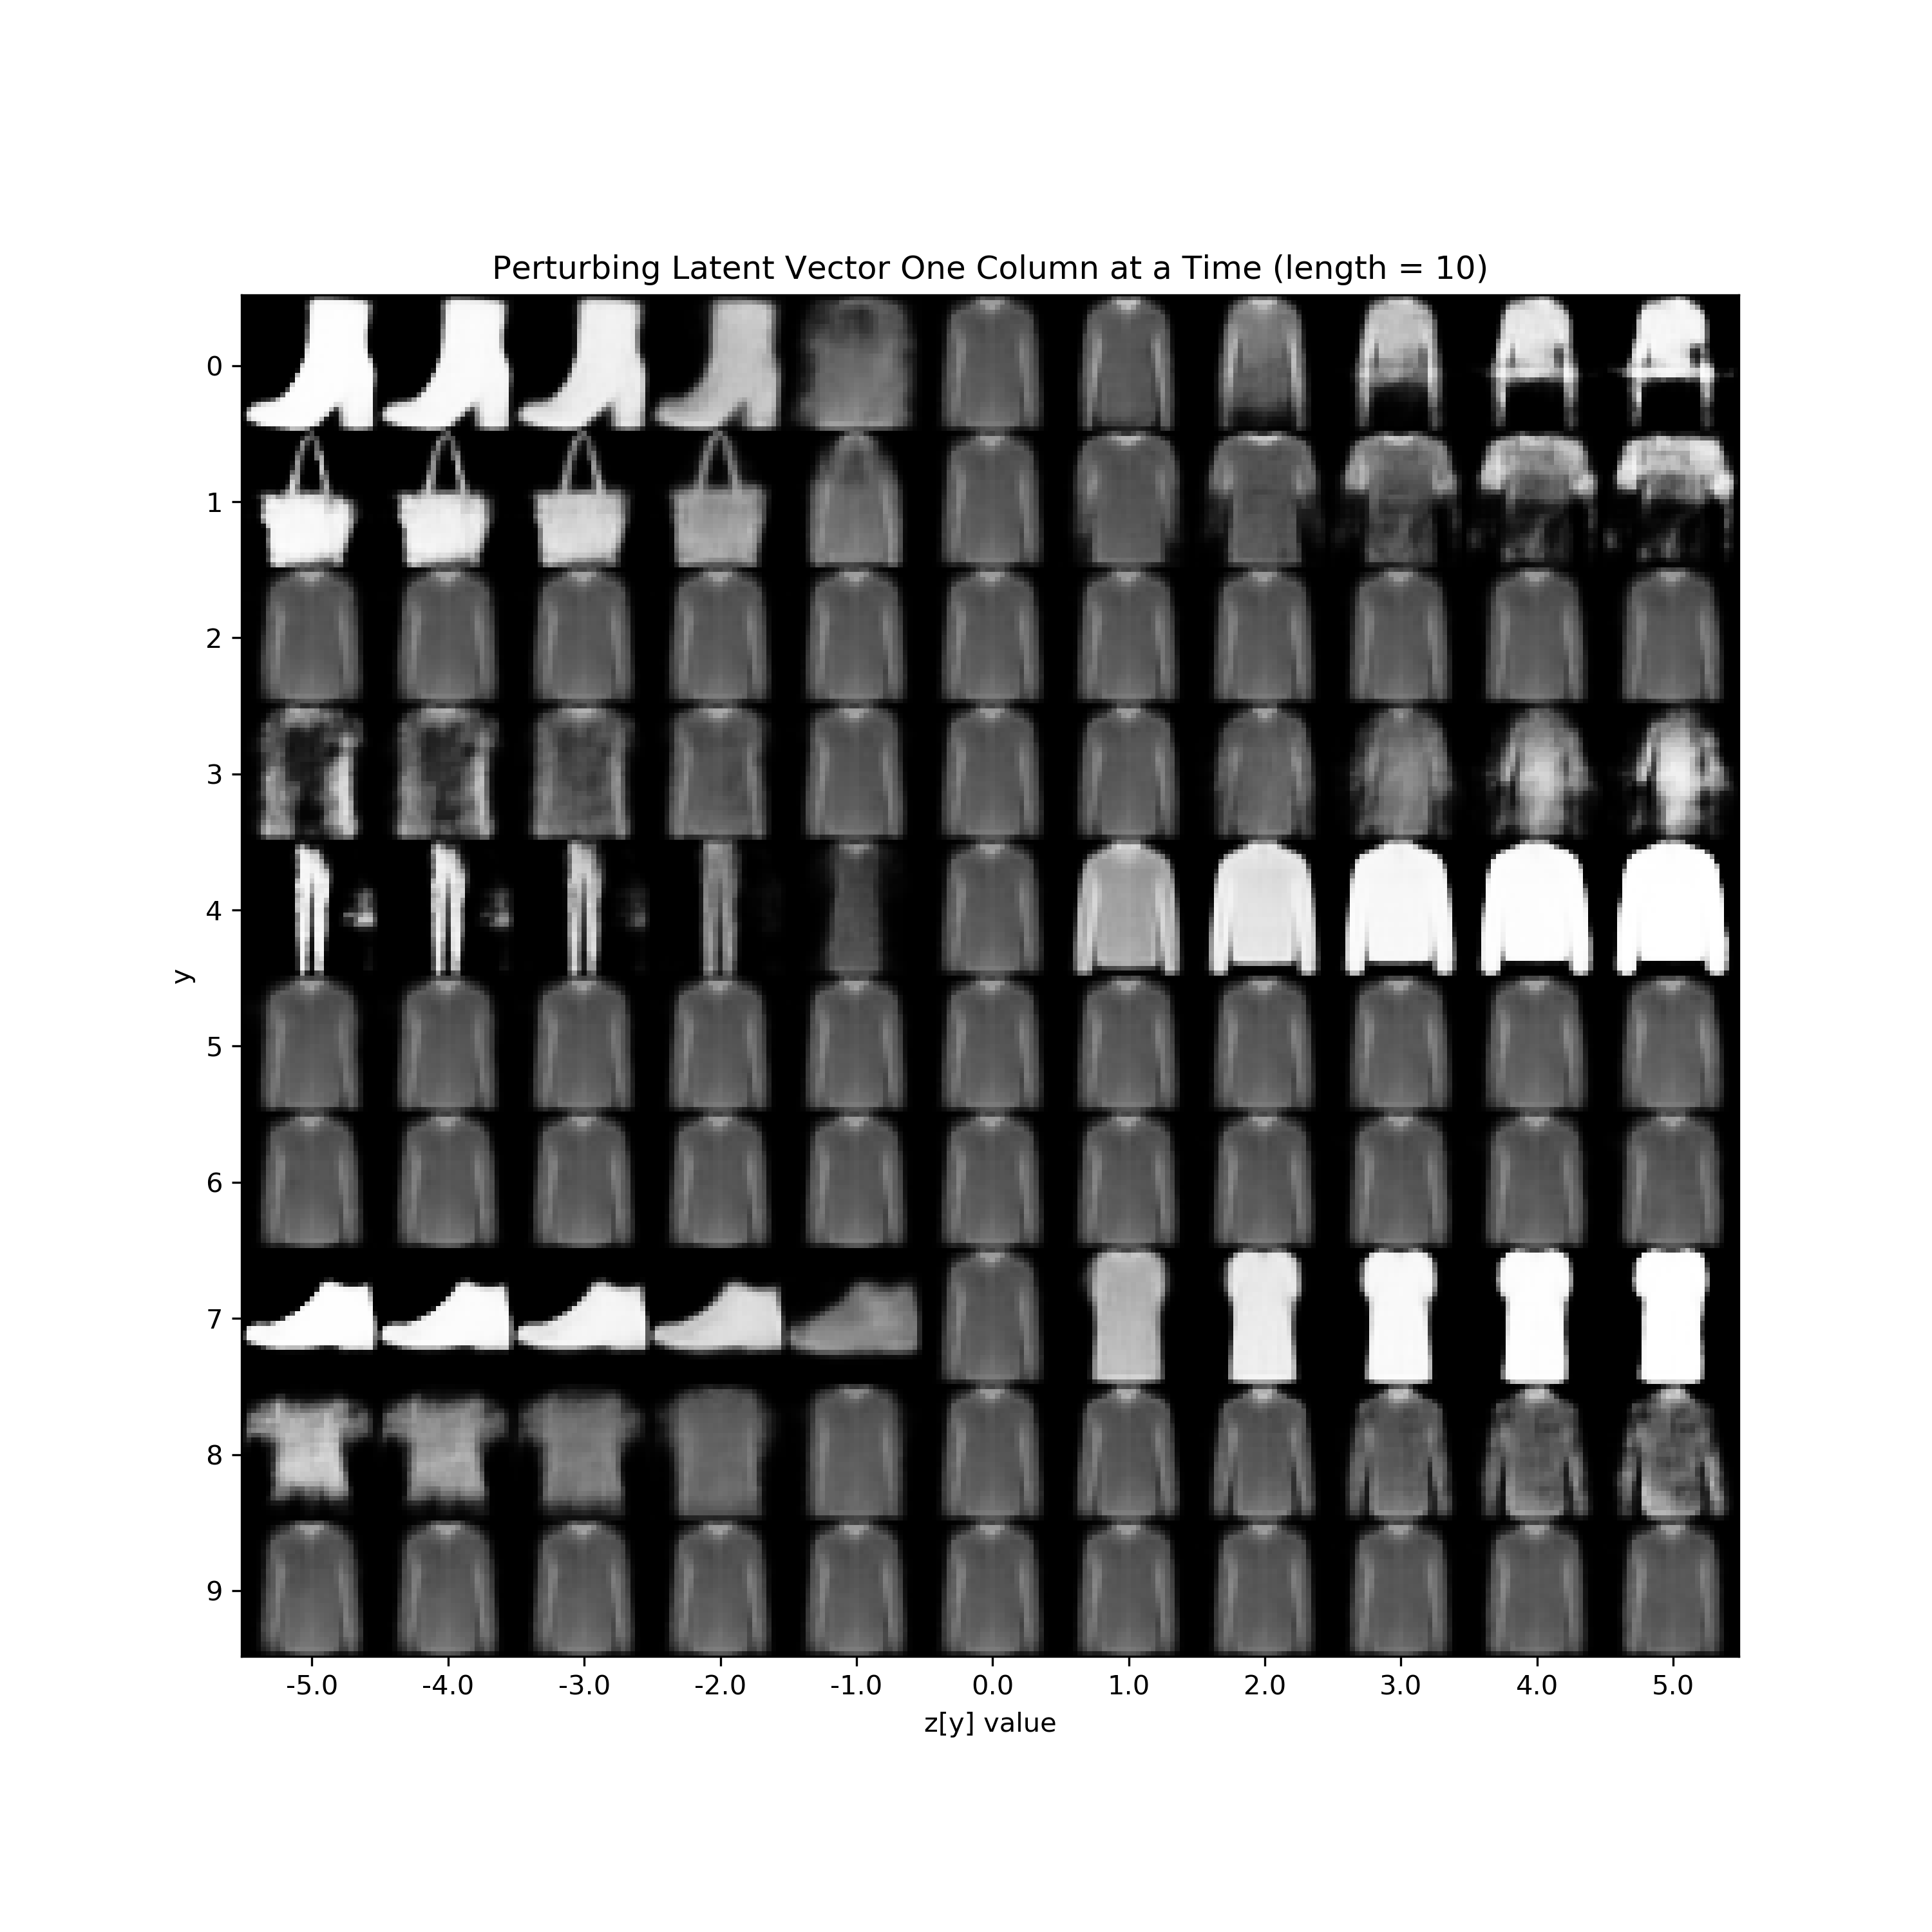
\includegraphics[width=\linewidth]{task_5_clothes_kernel_5_kernels_32_latent_10.png}
    \caption{Clothes generated using VAE$_2$'s decoder after walking over each latent dimension iteratively.}
    \label{fig:task_5_clothes_kernel_5_kernels_32_latent_10}
  \end{figure}

  \begin{figure}
    \centering
    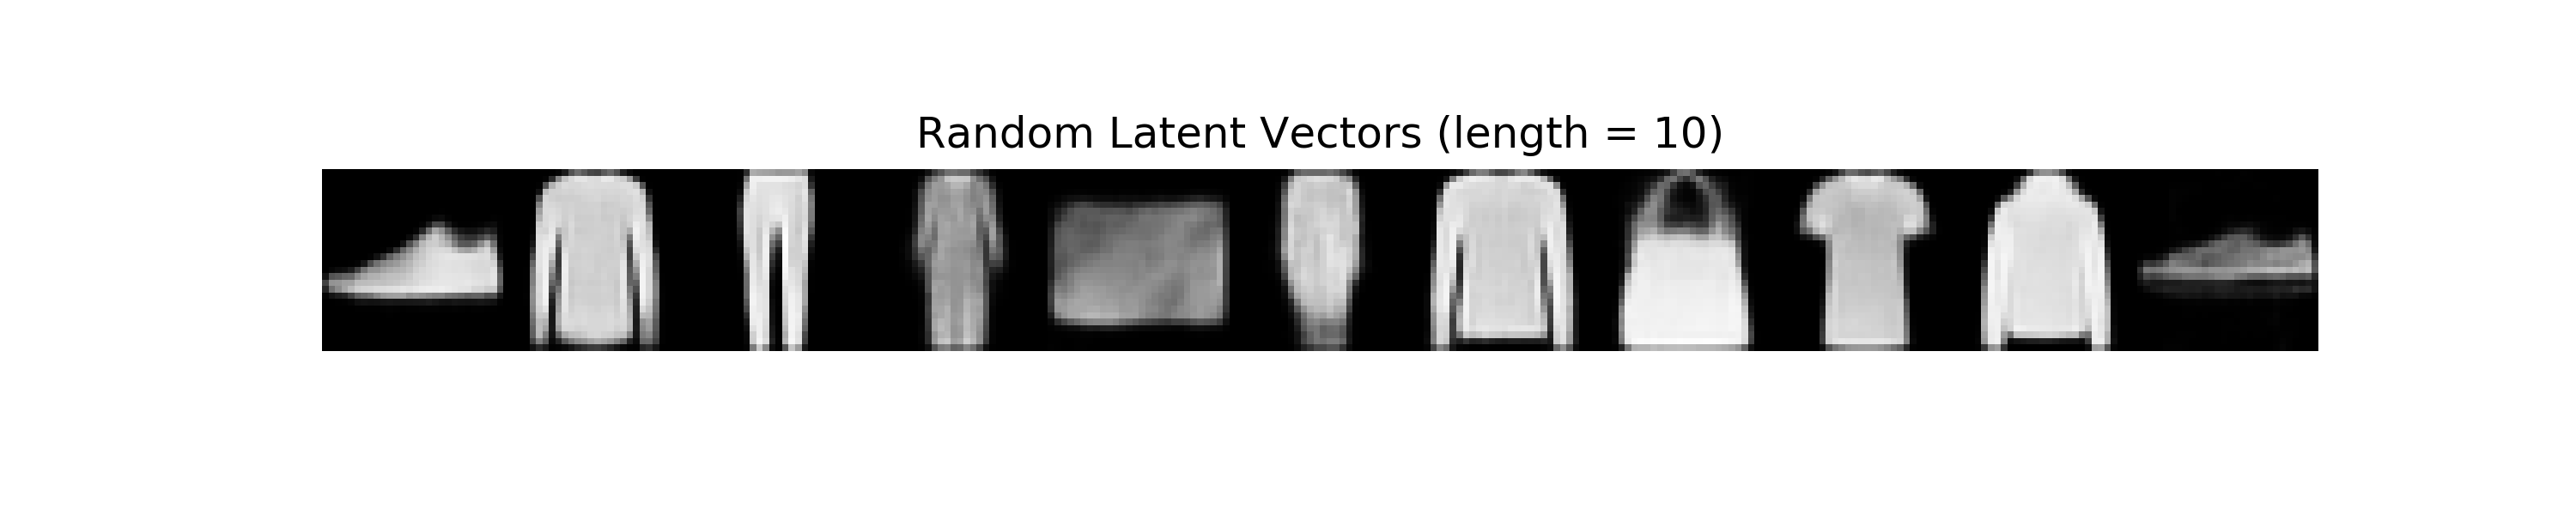
\includegraphics[width=\linewidth]{task_5_clothes_kernel_5_kernels_32_latent_10_examples.png}
    \caption{Clothes generated using VAE$_2$'s decoder using 11 randomly generated latent vectors.}
    \label{fig:task_5_clothes_kernel_5_kernels_32_latent_10_examples}
  \end{figure}

  \begin{table}[]
    \centering
    \caption{Loss across optimizers on VAE$_2$.}
    \label{tab:VAE_2}
    \begin{tabular}{|c|c|c|c|c|c|c|c|}
    \hline
     & SGD & RMSprop & Adagrad & Adadelta & Adam & Adamax & Nadam \\ \hline
    Mean Squared Error & 97.39 & 23.03 & 25.99 & 31.94 & 23.12 & \textbf{22.83} & 67.98 \\ \hline
    \end{tabular}
    \end{table}

\section{Conclusion}

The main factor that we were testing was each optimizer's ability to reach the lowest minimum with stock settings.
For most of the tasks performed here, Adamax was the clear winner, even if it was only marginally every single time.

In terms of classification, my convolutional neural network, MCNN, performed the best of all four classifiers
 tested, and did so by at least a 2.5\% margin. The only place it truly lacked in robustness was classifying shirts.

For the variational auto encoder, it seems that VAE$_1$ was more than sufficient in embedding Fashion-MNIST
 in its latent space with room to spare.
And it didn't prevent any of the optimizers from converging to a low loss.
Sometimes more isn't always better.

For future work, it would be worth rerunning the experiments we did here, except instead of changing
 the optimizer between runs, the hyperparameters of Adamax should instead be tweaked to see if any more performance could be gotten out of it.



\section{Running My Code}

Run ``python main.py $<$task\#$>$''. That's the driver file, the rest is the library.
Each task will run through $50$ epochs on each optimizer, graph the loss and accuracy curves of all of them, and
 plot the confusion matrix of the best one.

If there are problems with the environment, I've included two files to
 bootstrap an environment to run my code in.
``pip\_requirements'' can be used to create a pip virtual environment with
 the commands:
\begin{python}
  python3 -m venv env
  source env/bin/activate
  pip install -r pip_requirements.txt
\end{python}
Similarly, if using conda, use ``conda\_requirements'' with the command
\begin{python}
  conda create --name <env> --file conda_requirements.txt
\end{python}

\bibliographystyle{abbrv}

\end{document}